\chapter{Modellierung für Softwareentwicklungsprozesse}\label{sec:chapter6}
In diesem Kapitel wird ein Vergleich der Anwendbarkeit zwischen imperativer und deklarativer Modellierung für Softwareentwicklungsprozesse gezogen. Als Erstes wird dieser Vergleich in Kapitel 5.1 für das Softwareentwicklungsprozess Scrum durchgeführt. Hierfür wird zunächst in Kapitel 5.1 das der Modellierung zugrunde liegende Modell, das Softwareentwicklungsprozess Scrum, vorgestellt und für die Modellierung analysiert. Danach erfolgt die imperative Modellierung in der imperativen Prozessmodellierungssprache BPMN und anschließend die deklarative Modellierung in der deklarativen Prozessmodellierungssprache ConDec. Danach erfolgt der Vergleich zwischen den beiden Modellen.\newline
Der zweite Softwareentwicklungsprozess, welcher in diesem Kapitel in imperativer und deklarativer Prozessmodellierungssprache verglichen werden soll, ist der Open Unified Process (Open UP). Auch hier erfolgt zunächst eine kurze Einführung in den Open UP in Kapitel 5.2, bevor dieser in Kapitel 5.2.1 analysiert wird, damit er in imperativer, bzw. deklarativer Prozessmodellierungssprache modelliert werden kann. Hiernach erfolgt der Vergleich zwischen den imperativen und deklarativen Prozessmodellen.\newline
Zuletzt werden noch für das V-Modell XT die Prozessmodelle erstellt und verglichen. Eine Einführung in das V-Modell XT erfolgt in Kapitel 5.3. In Kapitel 5.3.1 wird für dieses als Vorbereitung für die Modellierung eine Analyse durchgeführt und es erfolgt die Modellierung in imperativer und deklarativer Prozessmodellierungssprache. Anschließend erfolgt der Vergleich erfolgt hierzu.\newline
Kapitel 5.4 widmet sich dem Vergleich zwischen allen Modellen insgesamt. Hier werden die Ergebnisse der Vergleiche aus den vorigen drei Kapiteln zusammengefasst und es werden allgemeine Schlüsse gezogen.\newline


\section{Scrum}\label{sec:chapter6:Imperative Modellierung}

Der Begriff Scrum stammt aus dem Artikel "The New New Product Development Game", welchen Hirotaka Takeuchi und Ikujiro Nonaka im Harvard Business Review 1986 veröffentlicht haben. Sie beschrieben einen ganzheitlichen Ansatz, bei dem kleine, funktionsübergreifende Teams zusammen an einem gemeinsamen Ziel arbeiten. Dies verglichen sie mit der Scrum-Formation beim Rugby \cite{Pham2012,Takeuchi1986}. \newline
Bei Scrum handelt es sich um ein agiles Prozessmodell, welches seit Anfang 1990 für komplexe Entwicklungen verwendet wird. Agile Prozessmodelle werden den leichtgewichtigen Prozessmodellen zugeordnet \cite{Hanser2010, Lacey2012}. Einen ersten Überblick über das Scrum-Prozessmodell gibt Abbildung \ref{fig:Scrum}.
\begin{figure}[htp]
\begin{center}
  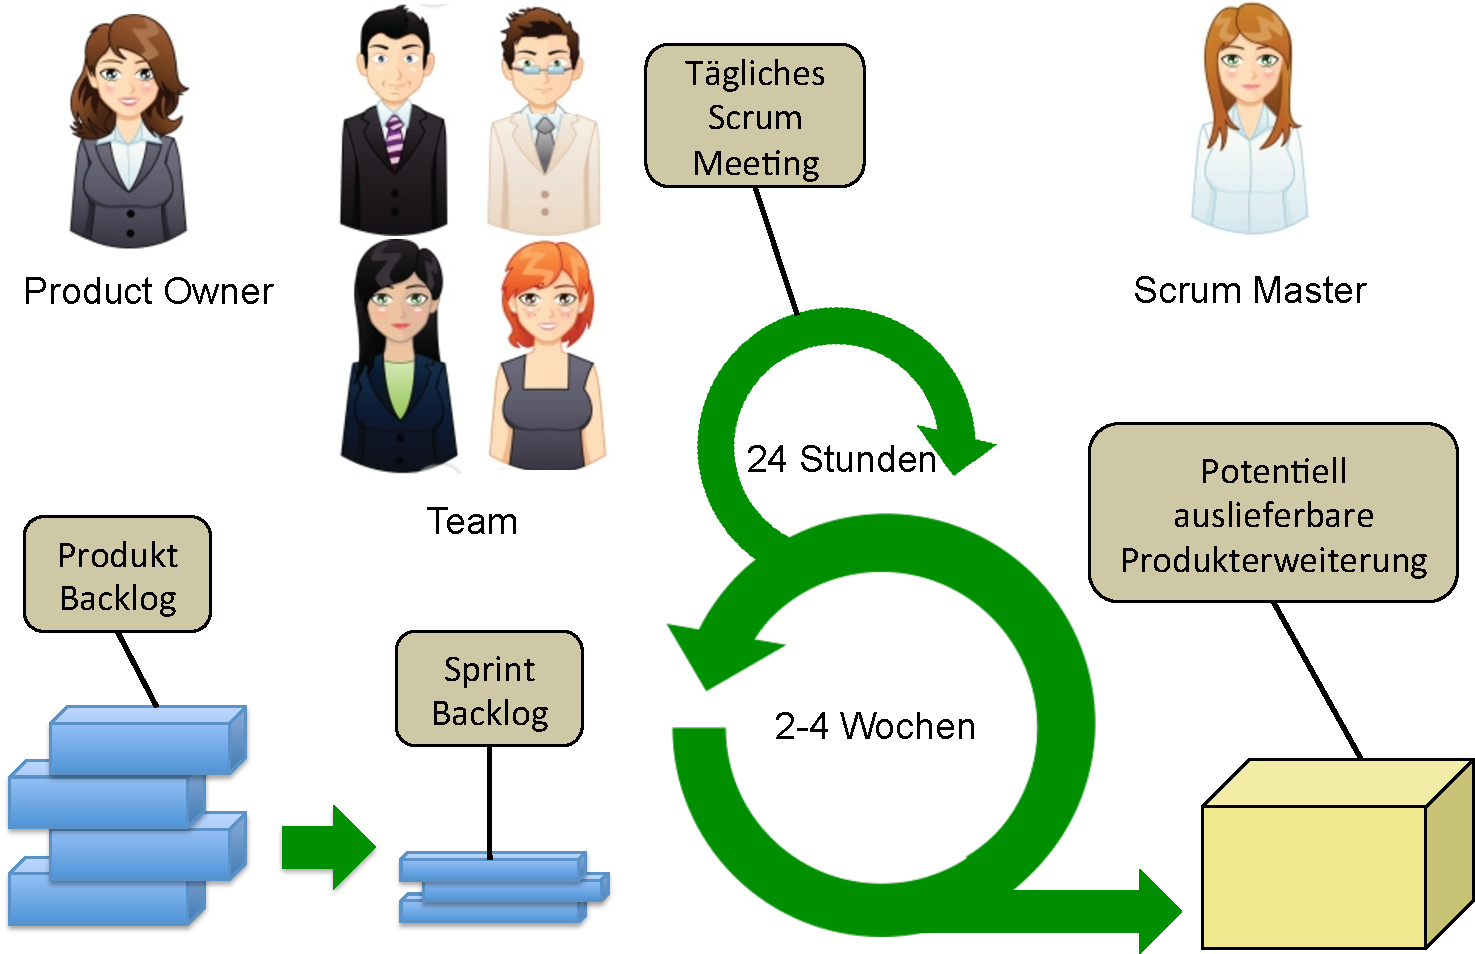
\includegraphics[scale=0.6]{Scrum} %pdf, jpg, png...
  \caption{Scrum Überblick nach \cite{scrum2008}}
  \label{fig:Scrum}
\end{center}
\end{figure}
Der genaue Ablauf im Scrum-Prozessmodell wird nachfolgend analysiert.

\subsection{Analyse Scrum}


Im Scrum-Prozessmodell gibt es nur drei verschiedene Rollen: Den \textit{Product Owner}, das \textit{Team} und den \textit{Scrum Master}. Sämtliche Verantwortlichkeiten innerhalb eines Projektes werden hierbei auf diese drei Rollen aufgeteilt \cite{Schwaber2004}. \newline

Der Procuct Owner ist verantwortlich, die Interessen aller am Projekt beteiligten Personen zu vertreten. Neben der Budgetierung des Projektes erstellt er  Releasepläne und fertigt den \textit{Produkt Backlog} an, welcher eine Liste mit funktionalen und nicht-funktionalen Anforderungen darstellt \cite{Schwaber2004, Pichler2010,Schwaber2007}. Weiterhin priorisiert er die Aufgaben, welche von den Entwicklern im \textit{Sprint} erledigt werden sollen, so dass die aktuell nützlichsten Elemente die höchste Priorität haben. Er erstellt eine Liste dieser Elemente, welche \textit{Sprint Backlog} genannt wird \cite{Henning2011, Schwaber2007,Pichler2010}. Der Procuct Owner ist ebenfalls zuständig für das Annehmen, bzw. Ablehnen der Arbeitsergebnisse \cite{eclipseScrum}. \newline

Die Teams bestehen bei Scrum für gewöhnlich aus fünf bis neun Mitgliedern und verwalten sich selbst. Ihre Tätigkeiten müssen erfolgreich sein, liegen aber in ihrer eigenen Verantwortung \cite{Pries2011, Wolf2011}. Alle Teammitglieder sind gemeinsam für den Erfolg eines jeden \textit{Sprints} und des gesamten Projektes zuständig \cite{Pichler2010}. \newline

Der Scrum Master ist für den gesamten Scrum-Prozess verantwortlich. Dies schließt die Vermittlung von Scrum-Inhalten (z.B. Schulungen) und die Implementation von Scrum in die Unternehmenskultur ein \cite{Pichler2010}. Er überwacht die Sprint- Tasks, um sicher zu gehen, dass der Sprint erfolgreich verläuft.\newline

Bei Scrum wird die Entwicklung in mehrere kurze Zyklen, also Iterationen eingeteilt. Eine einzelne Iteration wird bei Scrum \textit{Sprint} genannt \cite{Henning2011}. Die Dauer eines Sprints beträgt zwei bis vier Wochen. Am Ende eines jeden Sprints muss das Team ein lauffähiges Produkt abliefern \cite{Wolf2011}. Vor jedem Sprint findet ein \textit{Sprint Planning Meeting} statt, welches sich aus zwei Teilen zusammensetzt \cite{Pichler2010}. Im ersten Teil findet eine Planung des nächsten Sprints statt \cite{Lacey2012}. Hierfür präsentiert der Product Owner dem Team eine Liste der Product Backlog-Elemente mit der aktuell höchsten Priorität \cite{Schwaber2004, Schwaber2007,Pichler2010}. Diese Liste wird \textit{Sprint Backlog} genannt \cite{Wolf2011}. Das Team hat die Möglichkeit, Fragen bezüglich Inhalt, Zweck, Bedeutung und Absichten der Sprint Backlog-Elemente zu stellen. Anschließend werden die einzelnen Elemente aus dem Sprint-Backlog in sogenannte \textit{Tasks} aufgeteilt, welche jeweils eine ideale Bearbeitungszeit von zwei bis vier Stunden haben, aber niemals länger als zwei Tage dauern sollten \cite{Wolf2011}. Das Team kann sich die Aufgaben eigenverantwortlich aufteilen und muss sich anschließend dem Product  Owner verpflichten, die Tasks bis zum Abschluss des Sprints zu erledigen \cite{Wolf2011, Keith2010,Pichler2010}.
Das Team trifft sich während des Sprints täglich in einem 15-minütigen Meeting, dem \textit{täglichem Scrum Meeting}. Dabei redet das Team über seinen Fortschritt und eventuelle Probleme bei seiner Arbeit \cite{Keith2010}. Hier muss jedes Teammitglied die nachfolgenden drei Fragen beantworten \cite{Wolf2011}:
   \begin{enumerate}
      \item Was habe ich seit gestern erreicht?
      \item Was werde ich heute erreichen?
      \item Was blockiert mich?
      \end {enumerate}
      
\subsection{Imperative Modellierung Scrum}

Abbildung \ref{fig:ScrumImperativ} zeigt die imperative Modellierung von Scrum. Im Prozess gibt es die drei verschiedenen Rollen Product Owner, Team und Scrum Master, was im Prozessmodell durch drei verschiedene Swimlanes dargestellt ist. Manche Aktivitäten werden auch von mehreren Rollen ausgeführt. Da dies jedoch in BPMN nicht darstellbar ist, werden die entsprechenden Aktivitäten nachfolgend immer dem Hauptakteur zugeteilt.\newline
Parallel zu allen anderen Aktivitäten des Teams und des Product Owners muss der Scrum Master stets den Scrum-Prozess managen. Dies wird im Prozessmodell durch das Parallele Gateway dargestellt. \newline
Der Product Owner schätzt als erste Aktivität den Product Backlog ab. Anschließend priorisiert er den Product Backlog und erstellt parallel dazu die Releasepläne. \newline
Wenn alle zwei bis vier Wochen ein neuer Sprint beginnt, was hier durch ein Zeitereignis dargestellt ist, so wird zuerst das Sprint Planning Meeting durchgeführt. Dies ist hier als Unterprozess in Abbildung \ref{fig:ScrumImperativUnter} dargestellt. Zunächst priorisiert der Product Owner die Anforderungen, welche während des Sprints erledigt werden müssen, und erstellt danach den Sprint Backlog. Anschließend teilt sich das Team selbstständig die Sprint Backlog-Elemente in Tasks ein.\newline
Im Anschluss findet ein Sprint-Rückblick statt (Abbildung \ref{fig:ScrumImperativ}) und der Product Owner veranstaltet ein Sprint Review Meeting.\newline
Das Team führt während des Sprints täglich ein 15-minütiges Scrum Meeting durch und jedes Teammitglied arbeitet eine Task nach der anderen ab. Dies wird hier als Schleife dargestellt: Solange noch weitere Tasks vorhanden sind, führt das Exklusive Gateway immer wieder zurück zur Aktivität \textit{Tasks abarbeiten}. Erst wenn keine weiteren Tasks mehr vorhanden sind, führt der Prozess weiter zum nächsten Entscheidungspunkt.\newline
Sind noch weitere Aufgaben im Product Backlog vorhanden, die noch erledigt werden müssen, so beginnt ein weiterer Sprint, was hier durch eine Rückschleife dargestellt ist. Ist jedoch schon der komplette Product Backlog abgearbeitet, so endet der Prozess hier.


\begin{sidewaysfigure}[htp]
\begin{center}
  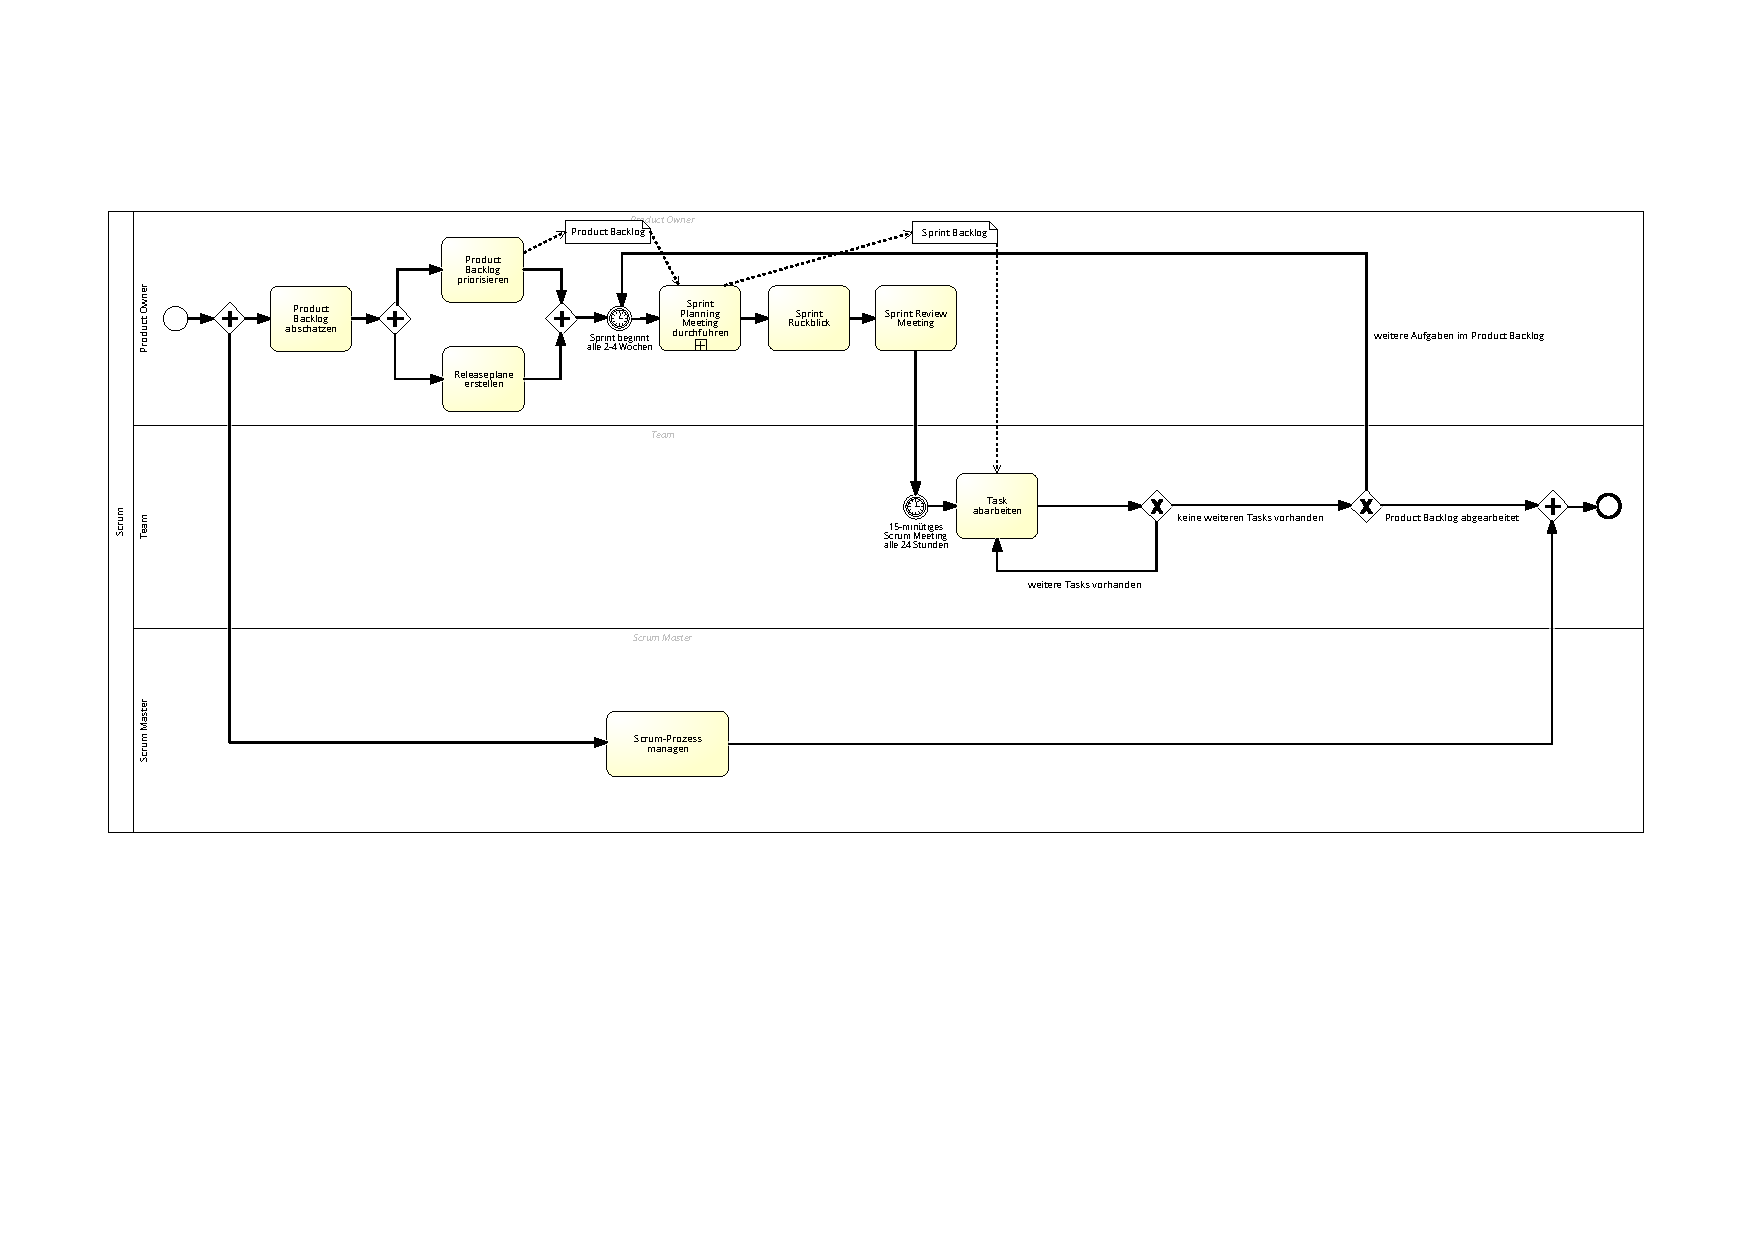
\includegraphics[width=\textwidth]{ScrumImperativ} %pdf, jpg, png...
  \caption{Imperative Modellierung Scrum}
  \label{fig:ScrumImperativ}
\end{center}
\end{sidewaysfigure}

\begin{figure}[htp]
\begin{center}
  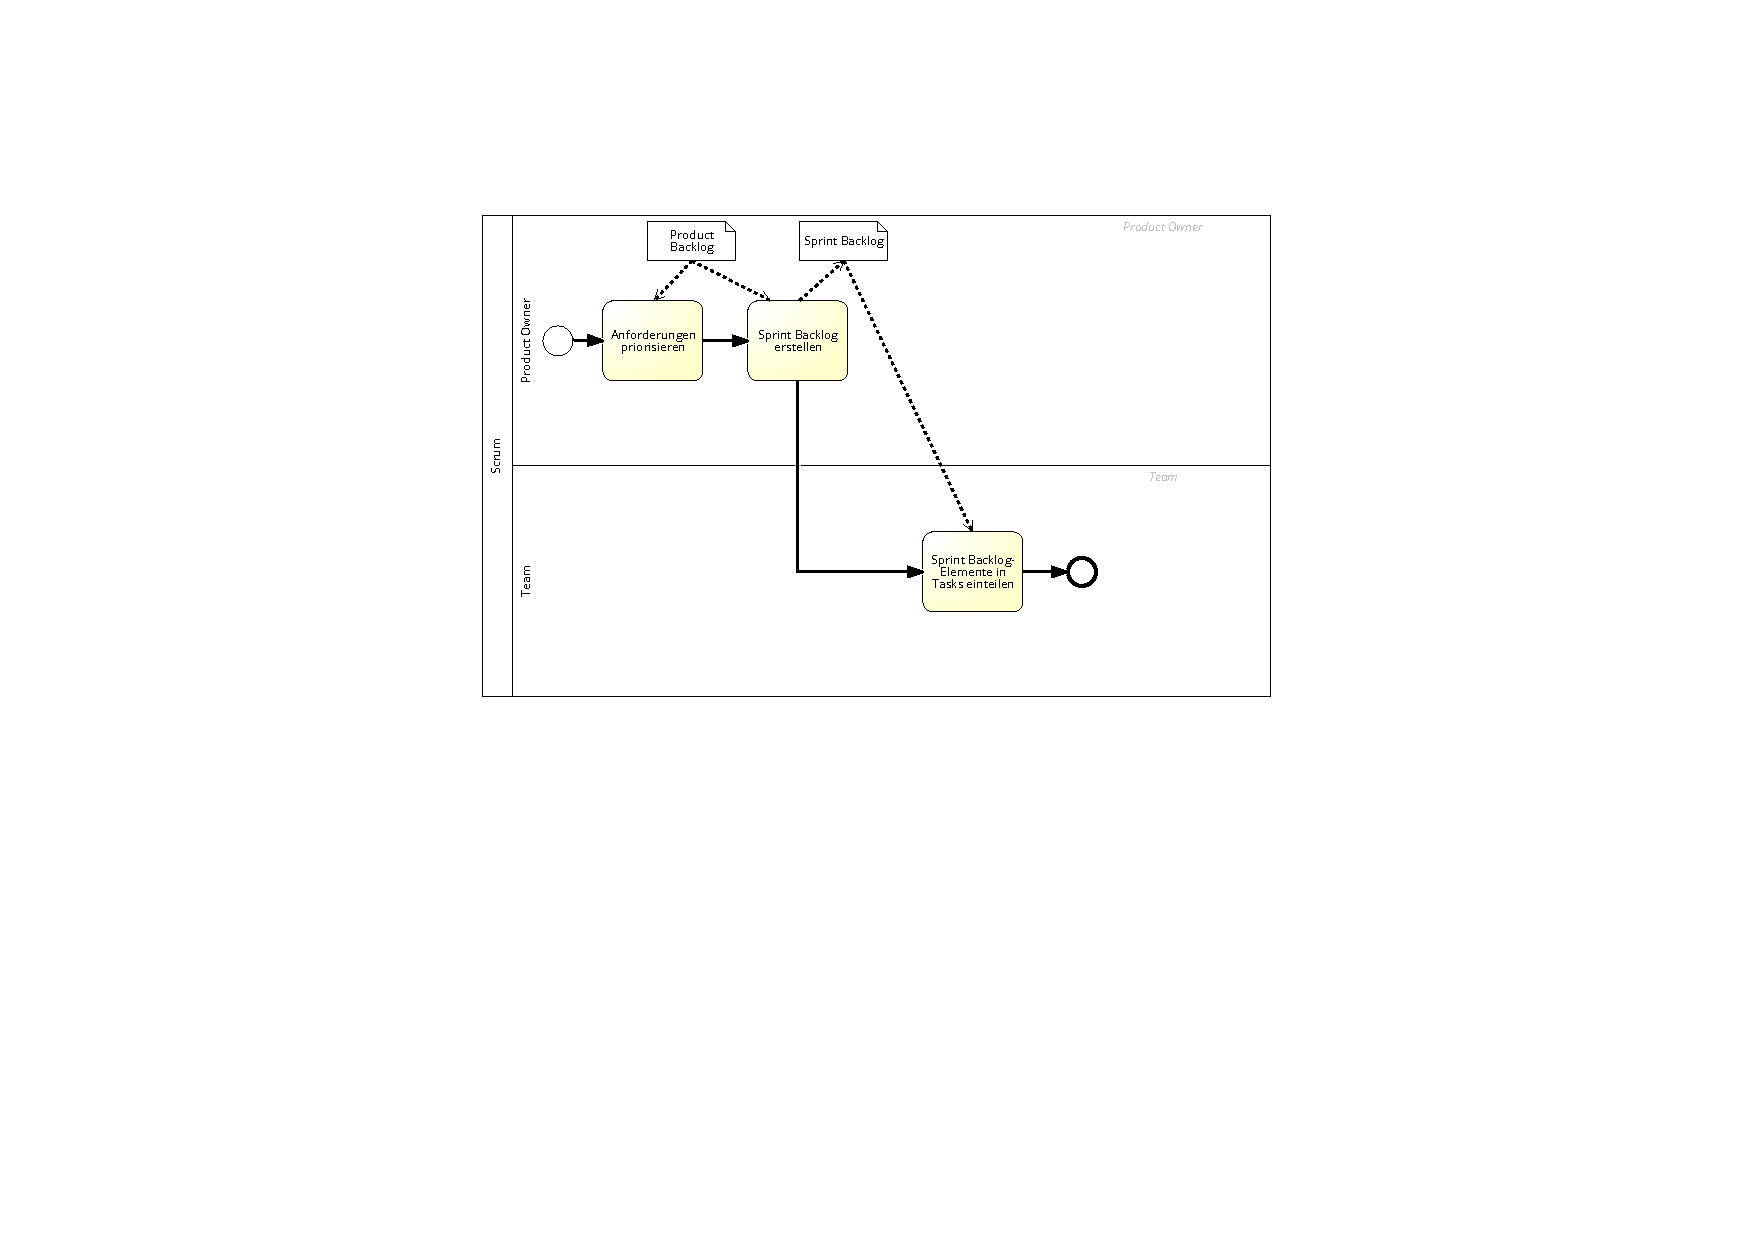
\includegraphics[scale=0.7]{ScrumImperativUnter} %pdf, jpg, png...
  \caption{Imperative Modellierung Scrum Unterprozess}
  \label{fig:ScrumImperativUnter}
\end{center}
\end{figure}
\clearpage

\subsection{Deklarative Modellierung Scrum}

Abbildung \ref{fig:ScrumDecHaupt} zeigt die deklarative Modelliereung von Scrum. Der Prozess beginnt mit der Aktivität "Product Backlog abschätzen". Dies ist hier durch das Init-Constraint gekennzeichnet. Weiterhin wird diese Aktivität im Prozess genau einmal ausgeführt was durch das Existenz Constraint dargestellt ist. Das Constraint \textit{succession} gibt an, dass die Aktivität \grqq Product Backlog abschätzen\grqq \ vor den Aktivitäten \grqq Product Backlog priorisieren\grqq \ und \grqq Releasepläne erstellen\grqq \ ausgeführt werden muss und dass die Aktivitäten \grqq Product Backlog priorisieren\grqq \ und \grqq Releasepläne erstellen\grqq \ auf jeden Fall nach \grqq Product Backlog abschätzen\grqq \ durchgeführt werden müssen. \grqq Product Backlog priorisieren\grqq \ und \grqq Releasepläne erstellen\grqq \ werden ebenfalls genau einmal ausgeführt, was durch das Existenz Constraint festgelegt wird.  \newline

Nach deren Ausführung muss die Aktivität \textit{alle 2-4 Wochen Sprint Planning Meeting durchfuehren} erfolgen. Der zugehörige Unterprozess ist in Abbildung \ref{fig:ScrumDecUnterprozess} zu finden. Hier sind die Aktivitäten \grqq Anforderungen priorisieren\grqq, \grqq Sprint Backlog erstellen\grqq \ und \grqq Sprint Backlog-Elemente in Tasks einteilen\grqq \ durch das Constraint \textit{precedence} miteinander verbunden, um die Einhaltung deren Reihenfolge nacheinander zu gewährleisten. Außerdem dürfen diese Aktivitäten pro Ausführung des Unterprozesses, also pro Prozessinstanz nur einmal ausgeführt werden.\newline
Nach der Ausführung der Aktivitäten des Unterprozesses Sprint Planning-Meeting durchführen, muss im Anschluß die Aktivität \grqq Sprint Rückblick\grqq \ durchgeführt werden. Dies wird durch das Constraint \textit{chain response} sichergestellt.Eine erneute Ausführung von \grqq alle 24 Stunden 15-minütiges Scrum-Meeting durchführen\grqq \ ist erst nach Durchführung von \grqq Sprint Rückblick\grqq \ möglich (Constraint \textit{alternate precedence}). Hierdurch wird eine Schleife modelliert, welche den immer wiederkehrenden Sprint simuliert.\newline
Die Aktivitäten \grqq alle 24 Stunden 15-minütiges Scrum-Meeting durchführen\grqq \ und \grqq Tasks abarbeiten\grqq \ können während des Sprints so oft wie nötig durchgeführt werden. Die Aktivitäten \grqq alle 24 Stunden 15-minütiges Scrum-Meeting durchführen\grqq \ und \grqq Tasks abarbeiten\grqq \ müssen jedoch nebeneinander ausgeführt werden, was durch das Constraint \textit{succession} beschrieben ist. \newline


\begin{figure}[htp]
\begin{center}
  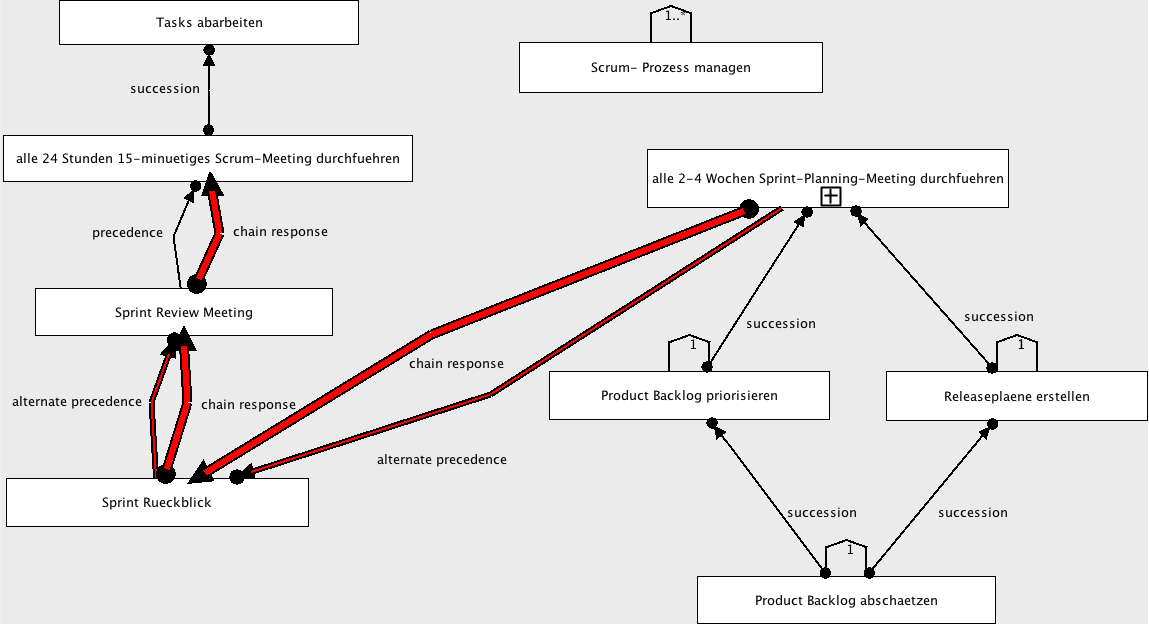
\includegraphics[width=\textwidth]{ScrumDecHaupt} %pdf, jpg, png...
  \caption{Deklarative Modellierung Scrum}
  \label{fig:ScrumDecHaupt}
\end{center}
\end{figure}



\begin{figure}[htp]
\begin{center}
  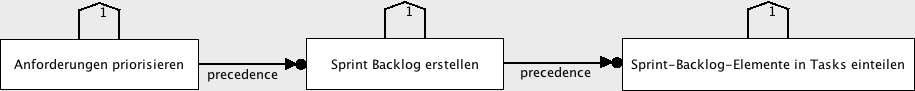
\includegraphics[width=\textwidth]{ScrumDecUnterprozess} %pdf, jpg, png...
  \caption{Deklarative Modellierung Scrum-Unterprozess Sprint-Planning-Meeting durchführen}
  \label{fig:ScrumDecUnterprozess}
\end{center}
\end{figure}
\clearpage

\subsection{Vergleich}

Der Vergleich zwischen den in der deklarativen Prozessmodellierungssprache ConDec und in der imperativen Prozessmodellierungssprache BPMN erstellten Scrum Prozessmodell wird im Folgenden anhand der in Kapitel 4 definierten Anforderungen durchgeführt. Auf Grund der dort definierten Vergleichskriterien wurden nachfolgend die Aktivitäten, die Anzahl der Constraints/Gateways, Anzahl der Sequenzflusselemente/Existenz, Anzahl unterschiedlicher Gateways/Constraints sowie die Summe der Elemente insgesamt in beiden Modellen gezählt. Weiterhin wurden die Aktivitäten gezählt, um später zwischen großen und kleinen Prozessmodellen vergleichen zu können. Hierdurch können im Folgenden die Modelle anhand der Vergleichskriterien miteinander verglichen werden. \newline
Wie Abbildung \ref{fig:ScrumExcel} entnommen werden kann, unterscheidet sich die Anzahl der Aktivitäten zwischen den in BPMN und ConDec modellierten Prozessmodellen nicht voneinander. In jedem Prozessmodell gibt es 12 Aktivitäten.\newline

\begin{figure}[htp]
\begin{center}
  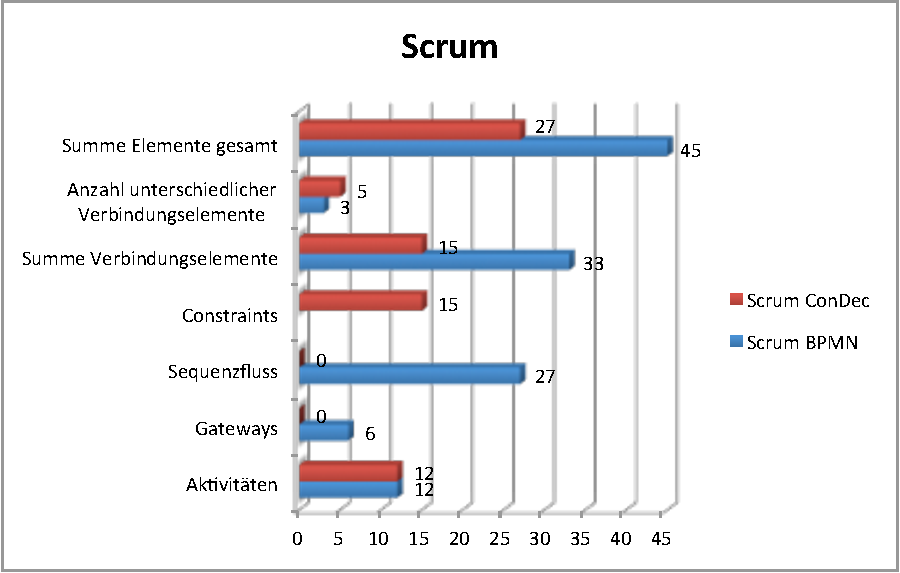
\includegraphics[scale=0.8]{ScrumExcel} %pdf, jpg, png...
  \caption{Vergleich der Anzahl der Elemente Scrum}
  \label{fig:ScrumExcel}
\end{center}
\end{figure}


Zudem braucht es in BPMN sechs Gateways und 26 Sequenzflusselemente, um den Ablauf des Metamodells darzustellen. Bei Verwendung von ConDec werden 13 Constraints (vier unterschiedliche) und sieben Existenz Constraints zur Darstellung der Abfolge der Aktivitäten benötigt. In BPMN werden sechs Gateways (zwei unterschiedliche) verwendet.\newline


Die syntaktische \textit{Richtigkeit} [A 1.1] kann bei beiden Modellierungssprachen eingehalten werden, da bei beiden Prozessmodellierungssprachen die Notationsregeln zur korrekten Darstellung des Prozessablaufes eingehalten werden können. Dies hat das Testen der beiden Modelle in Signavio, bzw. Declare bestätigt.\newline
Die semantische \textit{Richtigkeit} [A 1.2] lässt sich mit BPMN in Bezug auf Rollen und Artefakte besser einhalten, als mit ConDec. Da es bei ConDec keine Möglichkeit gibt, Rollen und Artefakte im Prozessmodell zu visualisieren fehlen diese Informationen. Die Rollen und Artefakte können zwar in Declare abgebildet werden, jedoch gibt es in ConDec hierfür keine Notationselemente, um Rollen und Artefakte im Prozessmodell selbst sichtbar zu machen. Aus diesem Grund müssen diese Informationen beim Modellieren weggelassen werden, was zur Folge hat, dass das im Metamodell beschriebene Verhalten nicht vollständig abgebildet werden kann und somit leidet auch der Nutzen des Modells.\newline
In Anbetracht der syntaktischen Richtigkeit [A 1.1] sind BPMN und ConDec gleich gut zur Modellierung geeignet. Bei Betrachtung der semantischen Richtigkeit ist  BPMN die geeignetere Modellierungssprache [A 1.2]. Somit erfüllt BPMN die \textit{Richtigkeit} besser, da es beiden Unterkriterien gerecht wird.\newline


Nur BPMN bietet die Möglichkeit, Artefakte im Prozessmodell zu visualisieren und lässt somit die Integration anderer Sichten in das Modell zu. Somit kann der Modellierungsgrundsatz des \textit{systematischen Aufbaus} [A 2.1] nur von BPMN eingehalten werden. Da ConDec dies nicht zulässt, können wichtige Informationen aus dem Metamodell nicht abgebildet werden. Somit erfüllt nur BPMN den Grundsatz des \textit{systematischen Aufbaus}.\newline 

Lediglich die mit BPMN erstellten Prozessmodelle können mit minimal relevanten Informationen erstellt werden. Der Grund dafür ist wiederum die fehlende Visualisierungsmöglichkeit von Rollen und Artefakten. Somit kann die \textit{Relevanz} [A 3.1] nur von BPMN eingehalten werden.\newline

Bei Untersuchung der \textit{Klarheit} lässt sich feststellen, dass sich die Anzahl der Sequenzflusselemente/Existenz Constraints zwischen BPMN (26) und ConDec (7) unterscheidet. Ebenfalls gibt es eine Differenz bei der Anzahl der Gateways (6)/Constraints (13) und der Anzahl der unterschiedlichen Gateways (2)/Constraints (4) zwischen BPMN und ConDec.\newline

Wie in Kapitel 4 bereits erwähnt [A 4.1], kann sich eine größere Anzahl an Gateways/Constraints negativ auf die Verständlichkeit auswirken. Hier ist die Anzahl bei ConDec mehr als doppelt so hoch wie bei BPMN. Zudem existiert im ConDec Modell keine eindeutige Start Aktivität [A 4.2], welche durch das Init-Constraint markiert ist. Dies liegt daran, dass mehrere Aktivitäten als Einstiegsaktivität in Frage kommen. Die möglichen Einstiegsaktivitäten sind jedoch nicht auf den ersten Blick ersichtlich. Dies steigert die Komplexität des ConDec Modelles. \newline
Das BPMN-Modell weißt nur im Hinblick auf die Anzahl von Sequenzflusselementen im Gegensatz zu Existenz Constraints einen höheren Wert auf. Wie in Kapitel 4 festgelegt wird die Anzahl Sequenzfluss/Existenz Constraints [A 4.1] einfach gewichtet und die Anzahl Gateways/Constraints und Anzahl unterschiedlicher Gateways/Constraints beim ConDec Modell doppelt [A 4.1] gewichtet. Somit weist das mit ConDec erstellte Modell in zwei jeweils doppelt gewichteten Punkten eine höhere Komplexität auf und das BPMN Modell nur in einem einfach gewichteten Punkt. Da noch die fehlende Startmarkierung bei ConDec [A 4.2] hinzu kommt, wird das mit ConDec erstellte Modell auf Grund der definierten Anforderungen in Kapitel 4 als komplexer eingestuft.
\newline
Somit ist hier BPMN in Bezug auf die \textit{Klarheit} geeigneter zum Modellieren als ConDec, da es die beiden unterkriterien [A 4.1] und [A 4.2] besser erfüllt.\newline

Die \textit{Wirtschaftlichkeit} unterscheidet sich bei den beiden Modellierungssprachen. Das mit BPMN erstellte Modell weist 26 Sequenzflusselemente auf und das mit ConDec erstellte Modell sieben Existenz Constraints. Bei ConDec hingegen werden mehr Constraints (13, 4 verschiedene) benötigt als Gateways (6, 2 verschiedene) bei BPMN. Hier gilt für das Kriterium [5.1] die gleiche Argumentation wie oben bei \textit{Klarheit, [4.1]}. Da die Anzahl Sequenzfluss/Existenz Constraints [A 5.1] einfach gewichtet und die Anzahl Gateways/Constraints und Anzahl unterschiedlicher Gateways/Constraints beim ConDec Modell doppelt [A 5.1] gewichtet wird, weist das ConDec Modell eine höhere Komplexität auf und der Modellierer hat somit einen höheren Aufwand beim Erstellen des Prozessmodelles.\newline
Aus diesem Grund erfüllt BPMN bei diesem Modell die \textit{Wirtschaflichkeit} besser als ConDec.\newline

Die \textit{Vergleichbarkeit} in Betracht des Ausführungsverhaltens der beiden Modelle wurde durch Testausführungen in den Modellierungstools Signavio und Declare gewährleistet [A 6.1].\newline
Bei BPMN weist das erstellte Modell insgesamt mehr Elemente auf. Während bei ConDec insgesamt 32 Elemente benötigt werden, werden zur Darstellung des gleichen Sachverhaltes bei BPMN 44 Elemente verwendet [A 6.2]. \newline
Bei ConDec müssen Informationen wie Rollen und Artefakte weggelassen werden, während sie in BPMN dargestellt werden können [A 6.3].\newline
Die \textit{Vergleichbarkeit} kann zwar in Bezug auf das Ausführungsverhalten von beiden Sprachen eingehalten werden [A 6.1]. BPMN weist jedoch insgesamt mehr Elemente auf [A 6.2] und ConDec kann die \textit{Vergleichbarkeit} in Bezug auf die Darstellbarkeit von Rollen und Artefakten nicht einhalten [A 6.3]. Somit kann ein Kriterium [6.2] von ConDec besser eingehalten werden. Kriterium [A 6.3] wird von BPMN besser erfüllt. Das Kriterium [6.1] kann von beiden eingehalten werden. Somit liegt hier keine der beiden Prozessmodellierungssprachen vorne.\newline

Abbildung \ref{fig:TabelleScrum} zeigt die Ergbenisse des Vergleichs von BPMN und ConDec nochmals in der Zusammenfassung. Somit liegt BPMN bei den Grundsätzen \textit{Richtigkeit}, \textit{systematischer Aufbau}, \textit{Klarheit} und \textit{Vergleichbarkeit} vorne, bei den Grundsätzen \textit{Wirtschaftlichkeit} und \textit{Relevanz} liegen BPMN und ConDec gleich auf. \newline

\begin{figure}[htp]
\begin{center}
  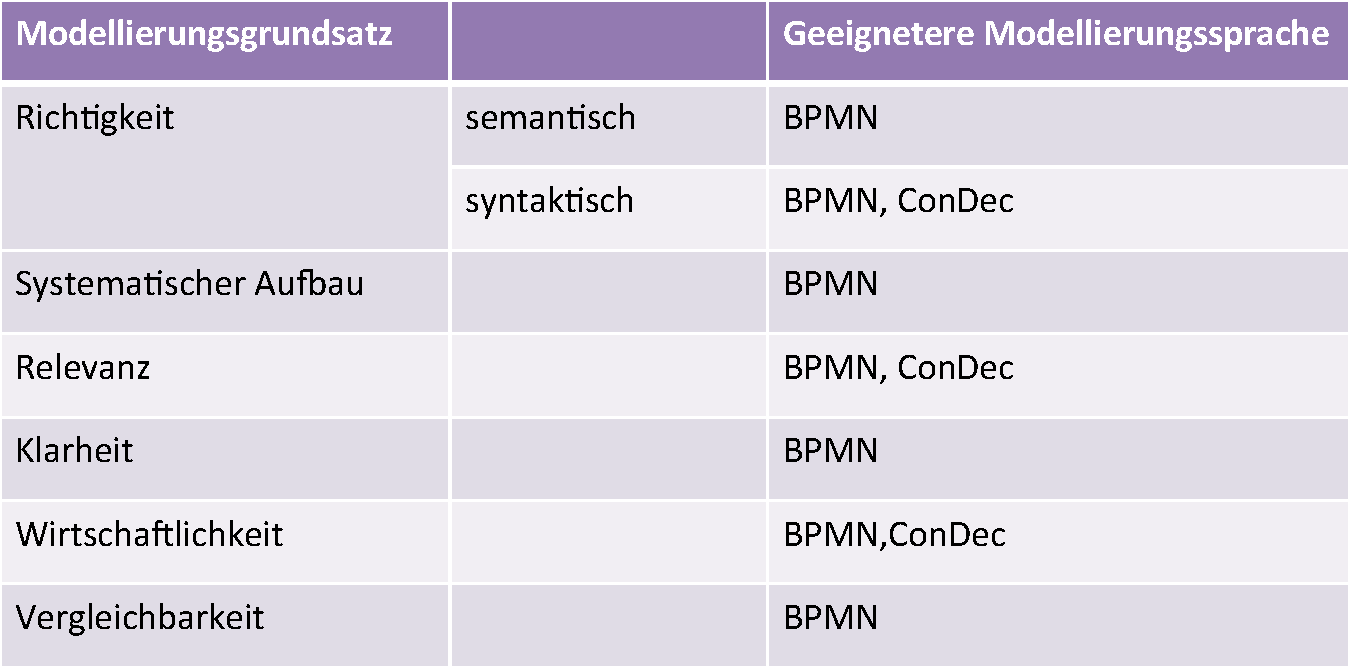
\includegraphics[scale=0.6]{TabelleScrum} %pdf, jpg, png...
  \caption{Zusammenfassung Vergleich Scrum}
  \label{fig:TabelleScrum}
\end{center}
\end{figure}




\section{Open Unified Process (Open UP)}


Der Open Unified Process, kurz Open UP ist eine frei zugängliche Variante des Rational Unified Process \cite{hauber2010}. Er ist Teil des Eclipse Process Frameworks. Open UP ist ein iterativer, inkrementeller und minimaler Prozess, aber dennoch vollständig und erweiterbar \cite{Gau2006, Basem2010}. Der Prozess ist minimal gehalten und bezieht somit nur die wesentlichen Inhalte ein. Er ist jedoch erweiterbar, da er mit weiteren Prozessfragmenten aufgestockt und dadurch nach Belieben zugeschnitten werden kann \cite{Wang2007}. Das Konzept des Open UP ist, sich bei einer Vergrößerung des Prozesses auf das Minimum zu beschränken, welches für das Projekt benötigt wird, anstatt zu versuchen große, überladene Prozesse zu verstehen und diese dann zu verkleinern \cite{ambler2012}.  \newline


Der Open UP wird im Folgenden analysiert.

\subsection{Analyse Open UP}

Open UP ist auf kleine Teams ausgerichtet, bei denen bei der Zusammenarbeit räumliche Nähe besteht. Die Teammitglieder haben hierbei die Freiheit, ihre eigenen Entscheidungen bezüglich ihren aktuellen Aufgaben und Prioritäten zu treffen, um die Anforderungen der Stakeholder zu erfüllen. Das Team trifft sich täglich, um über den aktuellen Status zu reden \cite{OpenUPProcess}.\newline
Es werden Rollen, Aufgaben, Artefakte und Ebenen in Open UP definiert. Dies soll ermöglichen, dass verschiedene Sichten, die sich in ihrem Detaillierungsgrad unterscheiden, auf das Projekt möglich sind \cite{freudenreichevaluierung}. Einen ersten Überblick über Open UP gibt Abbildung \ref{fig:openup}.

\begin{figure}[htp]
\begin{center}
  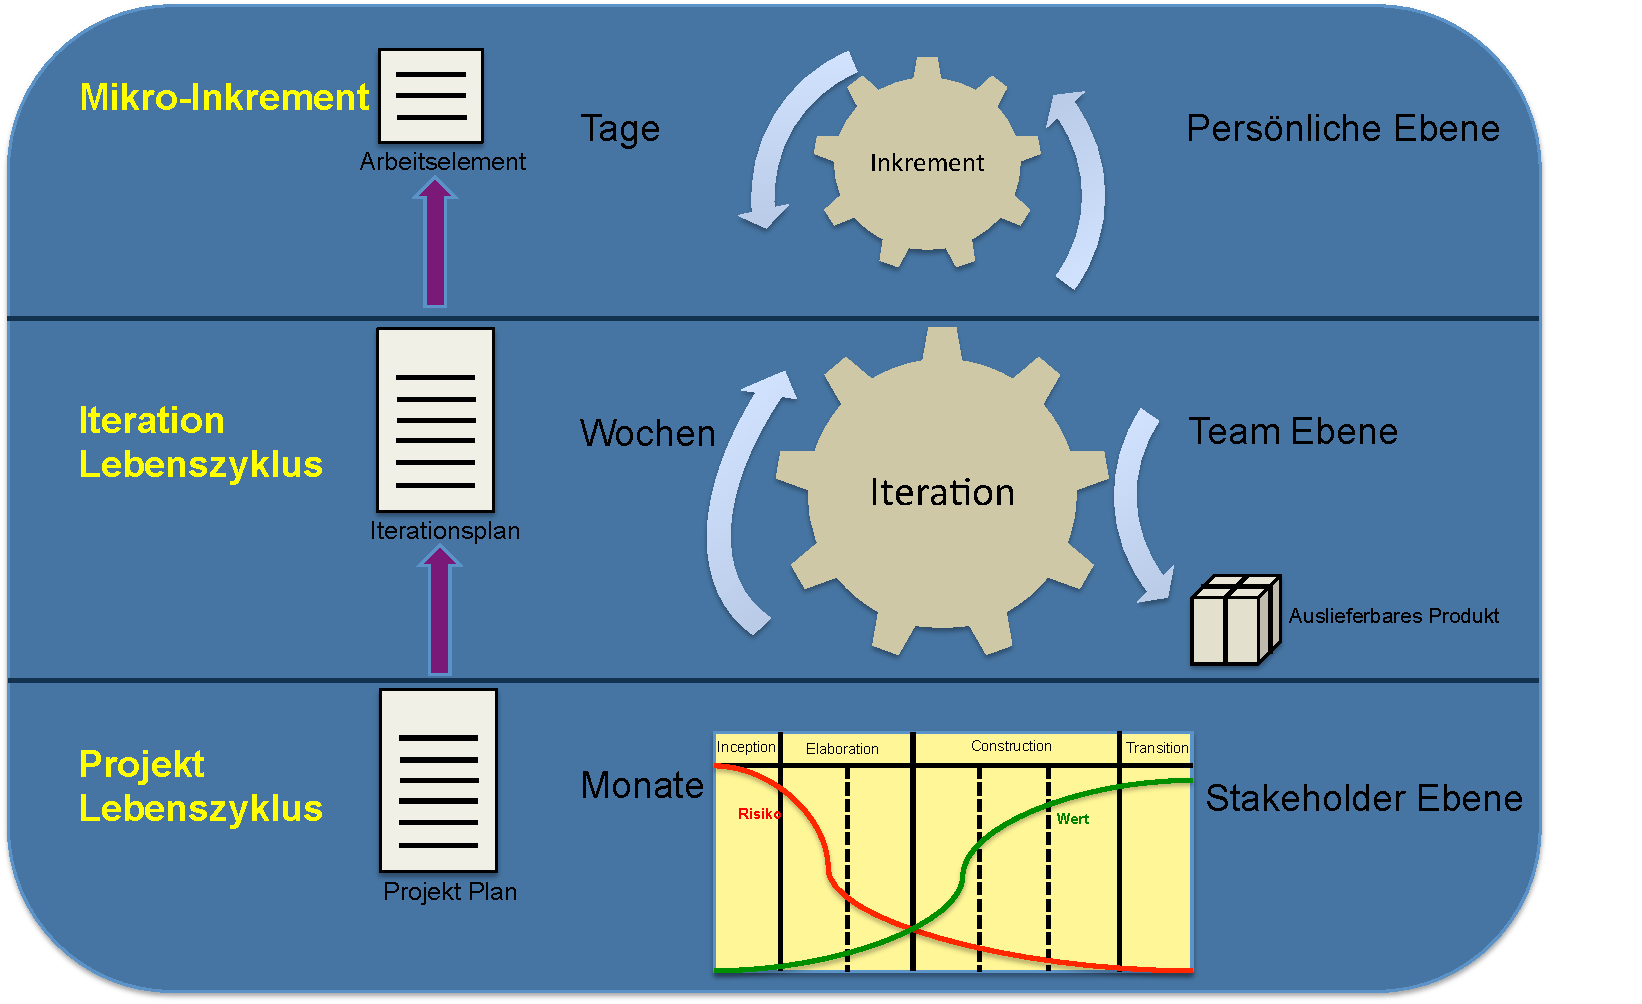
\includegraphics[width=\linewidth]{openup} %pdf, jpg, png...
  \caption{Open UP Überblick nach \cite{eclipseopenup}}
  \label{fig:openup}
\end{center}
\end{figure}

Auf der persönlichen Ebene teilen sich die Teammitglieder ihre Arbeit in \textit{Mikro-Inkremente} ein (Abbildung \ref{fig:openup}). Diese stellen das Ergebnis von Stunden, bzw. wenigen Tagen Arbeit dar. Die Arbeit entwickelt sich somit ein Mikro-Inkrement weiter und der Fortschritt kann Tag für Tag nachvollzogen werden. Die Teammitglieder teilen ihre Fortschritte täglich miteinander, was die Arbeitstransparenz und das Vertrauen erhöht und die Teamarbeit fördert \cite{eclipseopenup}. \newline

Auf der Team-Ebene wird das Projekt in Iterationen unterteilt (Abbildung \ref{fig:openup}), welche einen Zeitraum von mehreren Wochen umfassen. Das Ziel ist es, am Ende eines Iterationszyklus ein funktionierendes Softwareinkrement zu haben. Dieses Inkrement stellt eine Version des Softwaresystems dar welche zusätzliche oder verbesserte Funktionalitäten besitzt als die vorherige Version \cite{Basem2010}.  In jeder Iteration wird ein Iterationsplan angefertigt,  der vorgibt, was in dieser Iteration geliefert werden muss und auf welchen sich das Team verpflichten muss \cite{freudenreichevaluierung}.

Auf Stakeholder-Ebene wird diesen durch den \textit{Projektlebenszyklus} die Möglichkeit gegeben, die Projektfinanzierung, den Umfang, das Risiko und andere Aspekte des Prozesses zu kontrollieren (Abbildung \ref{fig:openup}).
Der Open UP teilt den \textit{Projektlebenszyklus} in die vier Phasen \textit{Inception}, \textit{Elaboration}, \textit{Construction} und \textit{Transition} ein, über welche Abbildung \ref{fig:Phasen} einen Überblick gibt \cite{eclipseopenup}.

\begin{figure}[htp]
\begin{center}
  \includegraphics[width=\linewidth]{Lebenszyklusopenup} %pdf, jpg, png...
  \caption{Phasen Open UP nach \cite{eclipseopenup}}
  \label{fig:Phasen}
\end{center}
\end{figure}


In jeder Phase finden eine oder mehrere Iterationen statt und werden mit einem Meilenstein abgeschlossen \cite{Basem2010}. In der Phase Inception ist dies der Zielsetzungmeilenstein, in der Phase Elaboration der Architekturmeilenstein, in der Phase Construction der Einsatzfähigkeitmeilenstein und in der Phase Transition der Produktreleasemeilenstein. Tabelle \ref{tab:tab1} zeigt die Abläufe den Iterationen in den einzelnen Phasen und die zugehörigen Zielstellungen.
\begin{longtable}{|p{7cm}|p{8cm}|}
\hline
Vorlagenmodell Iterationen & Zielsetzung der Phase \\
\hline
Inception Phase Iteration 
\begin {itemize}
\item Iteration starten 
 \item  Iteration planen und verwalten
 \item  Anforderungen festlegen und verfeinern 
  \end{itemize}
   &
  
  \begin {itemize}
\item Verstehen, was zu bauen ist
 \item Die wichtigsten Systemfunktionen verstehen 
\item Mindestens eine mögliche Lösung bestimmen
\item Kosten, Zeitplan und Risiken verstehen, welche mit dem Projekt verbunden sind
  \end{itemize}

 \\
\hline
 Elaboration Phase Iteration 
   \begin {itemize}
   \item Iteration planen und verwalten
   \item Anforderungen erheben und verfeinern
   \item Architektur definieren
   \item Lösung entwickeln
   \item Testlösung
   \item Laufende Aufgaben
   
  \end{itemize}

  & 
     \begin {itemize}
   \item Ein detaillierteres Verständnis der Anforderungen einholen
   \item Architektur designen, implementieren und validieren
   \item  Wesentliche Risiken mindern und genauen Zeitplan und Kostenschätzungen erstellen
    \end{itemize}
 \\
\hline
\hline
Construction Phase Iteration 
   \begin {itemize}
   \item Iteration planen und verwalten
   \item Anforderungen erheben und verfeinern
     \item Lösung entwickeln
   \item Testlösung
   \item Laufende Aufgaben

\end{itemize}

&
   \begin {itemize}
\item Komplettes Produkt iterativ entwickeln, welches am Ende bereit ist an seine Nutzer ausgeliefert zu werden
\item Entwicklungskosten minimieren und einen gewissen Grad an Parallelität erzielen 
\end{itemize}

 \\
\hline
Transition Phase Iteration 

   \begin {itemize}

 \item Iteration planen und verwalten
     \item Lösung entwickeln
   \item Testlösung
   \item Laufende Aufgaben

 \end{itemize}

 
  &
  
     \begin {itemize}
      \item Beta-Test, um zu überprüfen, dass die Erwartungen der Benutzer erfüllt sind 
     \item Zustimmung der Stakeholder einholen, dass Bereitstellung abgeschlossen ist
      \end{itemize}

\\

\hline

\caption{Iterationen und Zielstellungen der Phasen in Open UP \cite{eclipseopenup}}
\label{tab:tab1}
\end{longtable}






Abbildung \ref{fig:RollenOpenUp} gibt einen Überblick über die verschiedenen Rollen in Open UP. Die Rolle \textit{Analyst} stellt den Vertreter des Kunden und Endnutzer auf der Seite des Teams dar. Die Aufgaben des \textit{Analysten} bestehen aus dem Sammeln von Informationen von den Stakeholdern, um das Problem, welches es zu lösen gilt, zu verstehen. Weiterhin erstellt er Anforderungen und setzt Prioritäten für diese \cite{OpenUPProcess}.\newline
Der \textit{Tester} ist für sämtliche Testaktivitäten verantwortlich. Diese umfassen die Ermittlung, Festlegung, Umsetzung und Durchführung der erforderlichen Tests sowie die Protokollierung und Analyse der Ergebnisse \cite{OpenUPProcess}.
Der \textit{Entwickler} entwickelt einen Teil des Systems und muss hierbei sicherstellen, dass dieser in die Gesamtarchitektur passt. Er muss eventuell Prototypen des User-Interface anfertigen und anschließend die Komponenten implementieren, testen und integrieren \cite{OpenUPProcess}.\newline
Der \textit{Architekt} ist für die Definition der Software-Architektur verantwortlich, d.h. er trifft alle wichtigen technischen Entscheidungen, die die gesamte Entwicklung und Umsetzung des Systems betreffen \cite{OpenUPProcess}.\newline
Der \textit{Projekt Manager} führt die Planung des Projektes durch, koordiniert die Zusammenarbeit zwischen allen Beteiligten und achtet darauf, dass das Projektteam die Erfüllung der Projektziele stets im Auge behält \cite{OpenUPProcess}.\newline
Die Rolle des \textit{Stakeholders} schließt alle Interessengruppen ein, deren Ansprüche durch das Projekt erfüllt werden müssen. \newline

\begin{figure}[htp]
\begin{center}
  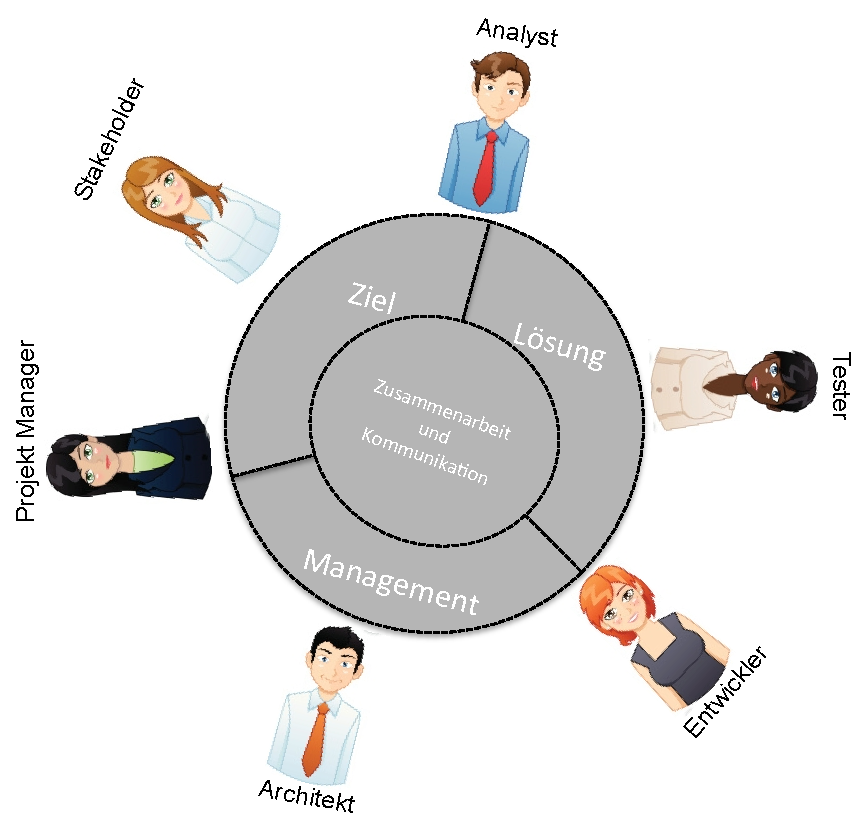
\includegraphics[scale=0.6]{RollenOpenUp} %pdf, jpg, png...
  \caption{Rollen in Open UP nach \cite{openup}}
  \label{fig:RollenOpenUp}
\end{center}
\end{figure}

Eine Task bezeichnet in Open UP die Arbeitseinheit einer Rolle, welche von dieser durchgeführt werden soll. Insgesamt gibt es 18 Tasks, die von den verschiedenen Rollen entweder als Hauptakteur (der Verantwortliche für die Durchführung der Aufgabe) oder als zusätzlicher Akteur (Unterstützung und Bereitstellung von Informationen, die in der Task- Ausführung verwendet werden), durchgeführt werden. Hierdurch wird der kollaborative Charakter von Open UP gefestigt \cite{eclipseopenup}.

Ein Artefakt ist etwas, das hergestellt, modifiziert oder durch eine Task verwendet wird. Rollen sind 
für die Erstellung und Aktualisierung von Artefakten verantwortlich. Artefakte stellen eine Versionskontrolle während des gesamten Projektlebenszyklus dar. Die 17 Artefakte in Open UP gelten als die wesentlichen Artefakte, welche ein Projekt verwenden sollte, um produkt- und projektbezogene Informationen zu erfassen. Die Informationen müssen hierbei nicht mit formalen Artefakten festgehalten werden. Dies kann auch informell, z.B. durch White-Boards oder Meeting-Notizen geschehen. Es können die Open UP Artefakte oder eigene Artefakte verwendet werden \cite{eclipseopenup}.

\subsection{Imperative Modellierung Open UP}

Nachfolgend werden einzelne Abschnitte des Open UP in der imperativen Prozessmodellierungssprache BPMN modelliert.

 \subsubsection{Phasen Open UP}

In Abbildung \ref{fig:OpenUpPhasen} sind die vier Phasen des Open UP modelliert. Da jede Phase in Iterationen mehrmals durchlaufen werden kann, gibt es nach jeder Phase ein Exklusives Gateway, welches im Falle einer weiteren notwendigen Iteration zum Anfang der Phase zurückführt. Diese kann sodann erneut durchlaufen werden.

\begin{sidewaysfigure}[htp]
\begin{center}
  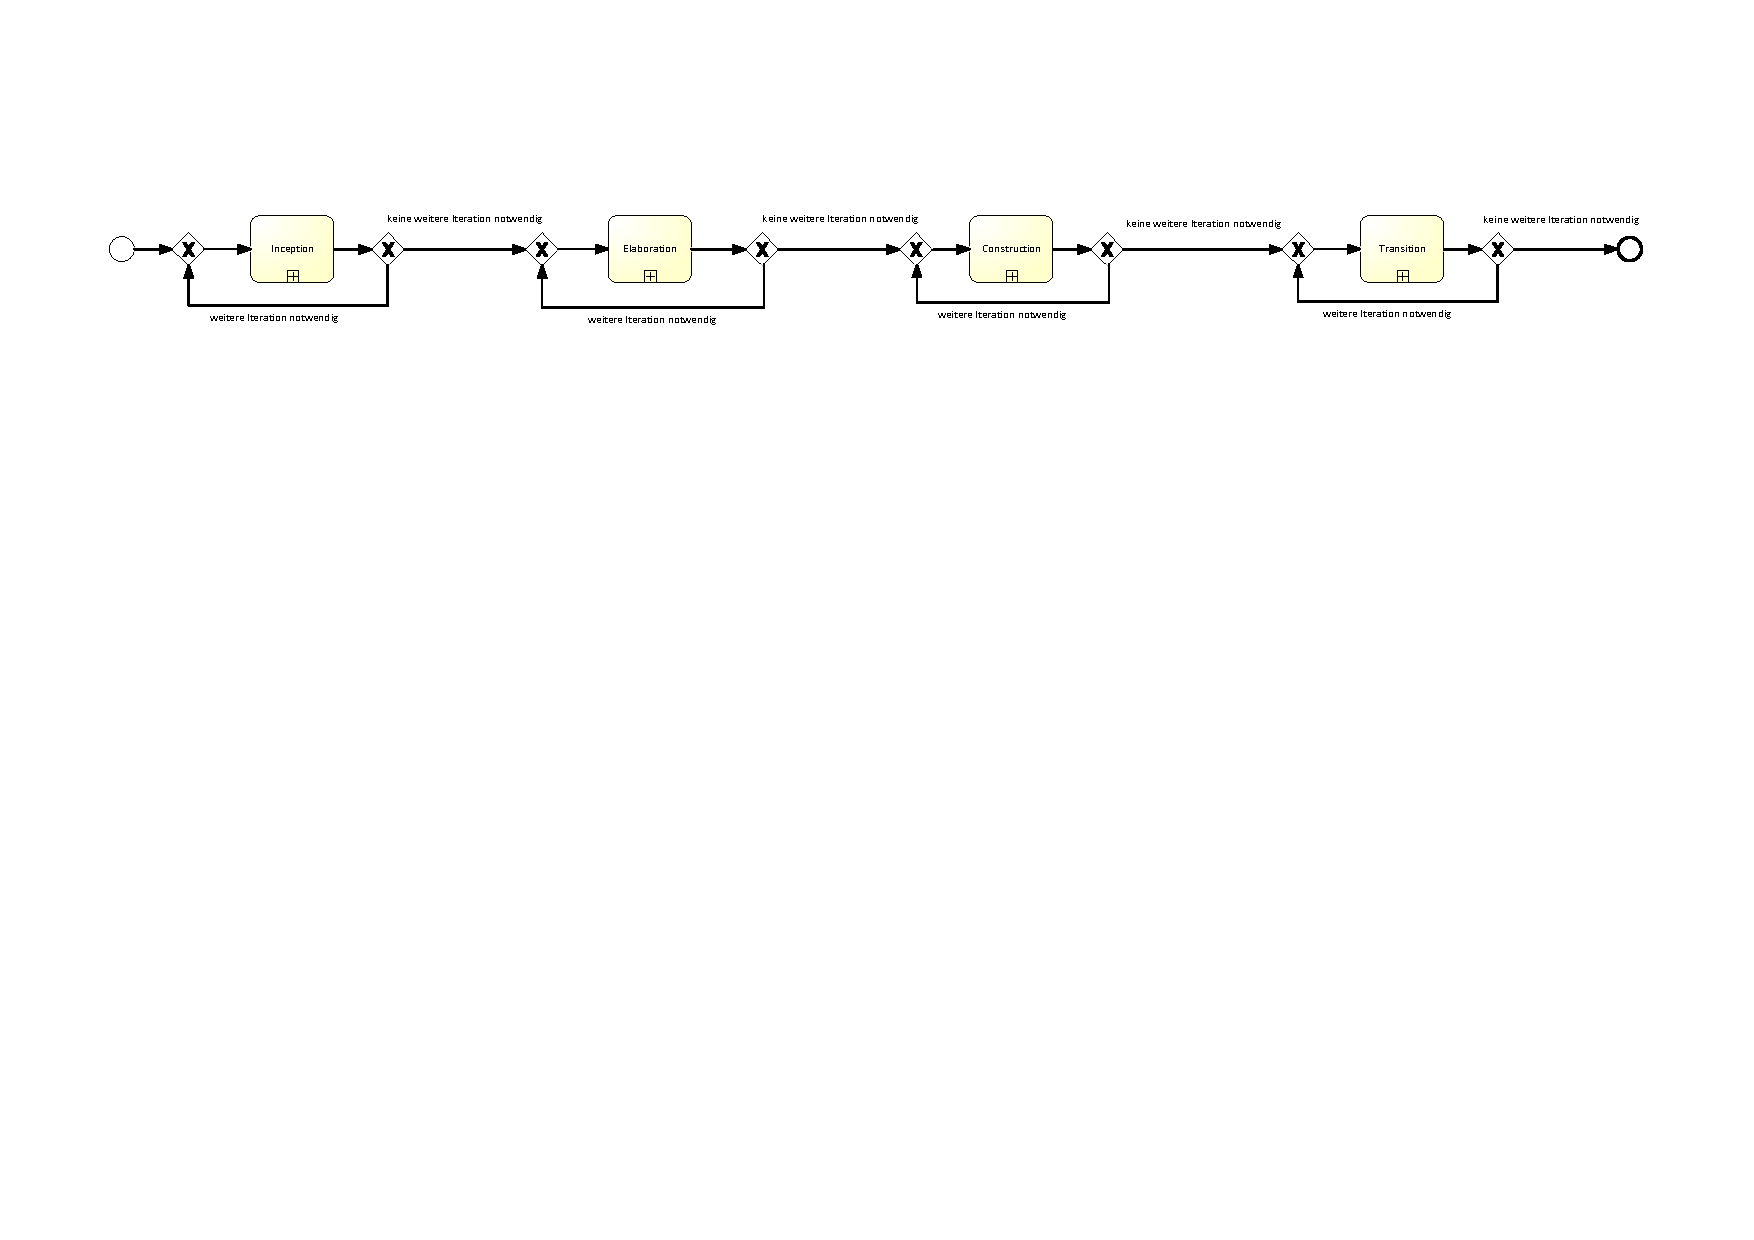
\includegraphics[width=\linewidth]{OpenUpPhasen} %pdf, jpg, png...
  \caption{Phasen Open UP- imperativ}
  \label{fig:OpenUpPhasen}
\end{center}
\end{sidewaysfigure}

Abbildung \ref{fig:OpenUpInception} zeigt die imperative Modellierung der Iteration Inception. Die Aktivität \grqq Projekt planen und managen \grqq \ kann parallel zu allen anderen Aktivitäten des Modells ausgeführt werden.\newline
Nach Ausführung der Aktivität \grqq Iteration planen\grqq \ werden die Aktivitäten \grqq Anforderungen identifizieren und aufbereiten\grqq \ und \grqq auf technisches Vorgehen einigen\grqq \ parallel zueinander ausgeführt.

\begin{figure}[htp]
\begin{center}
  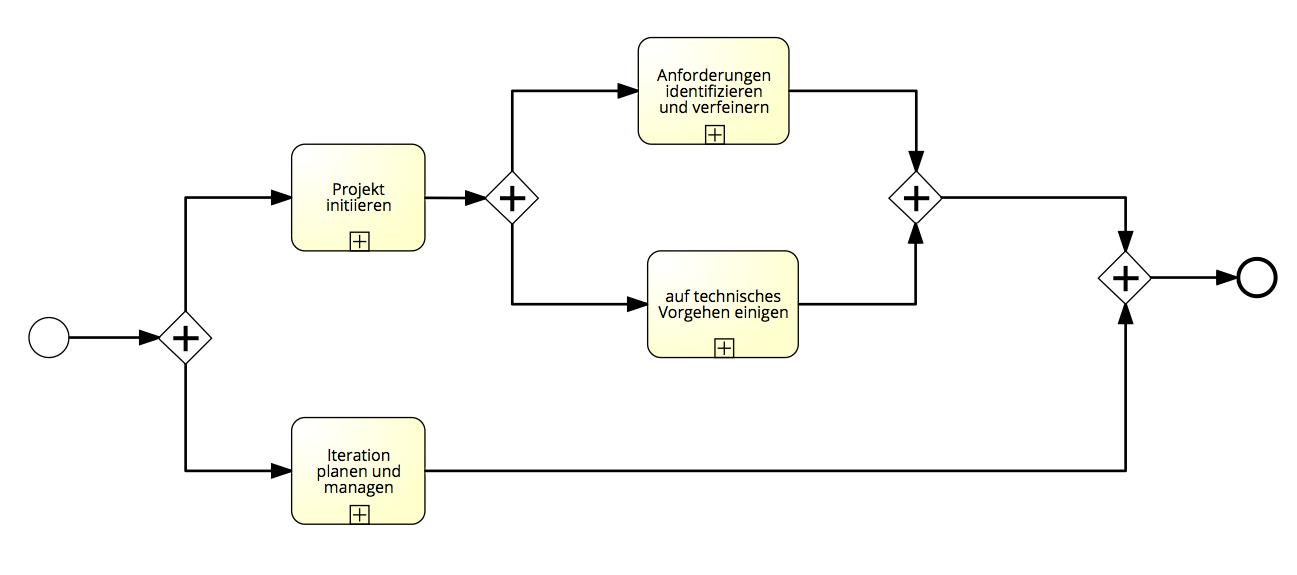
\includegraphics[scale=0.8]{OpenUpInception} %pdf, jpg, png...
  \caption{Phasen Open UP Unterprozess Inception- imperativ}
  \label{fig:OpenUpInception}
\end{center}
\end{figure}

In Abbildung \ref{fig:OpenUpElaboration} ist die imperative Modellierung der Iteration Elaboration abgebildet. Die sechs Aktivtäten \grqq Anforderungen identifizieren und verfeinern\grqq , \grqq Architektur entwickeln\grqq, \grqq Lösungsinkrement entwickeln\grqq, \grqq Lösung testen\grqq, \grqq Iteration planen und managen\grqq \ sowie \grqq weitere Aufgaben erledigen\grqq \ werden parallel zueinander ausgeführt.

\begin{figure}[htp]
\begin{center}
  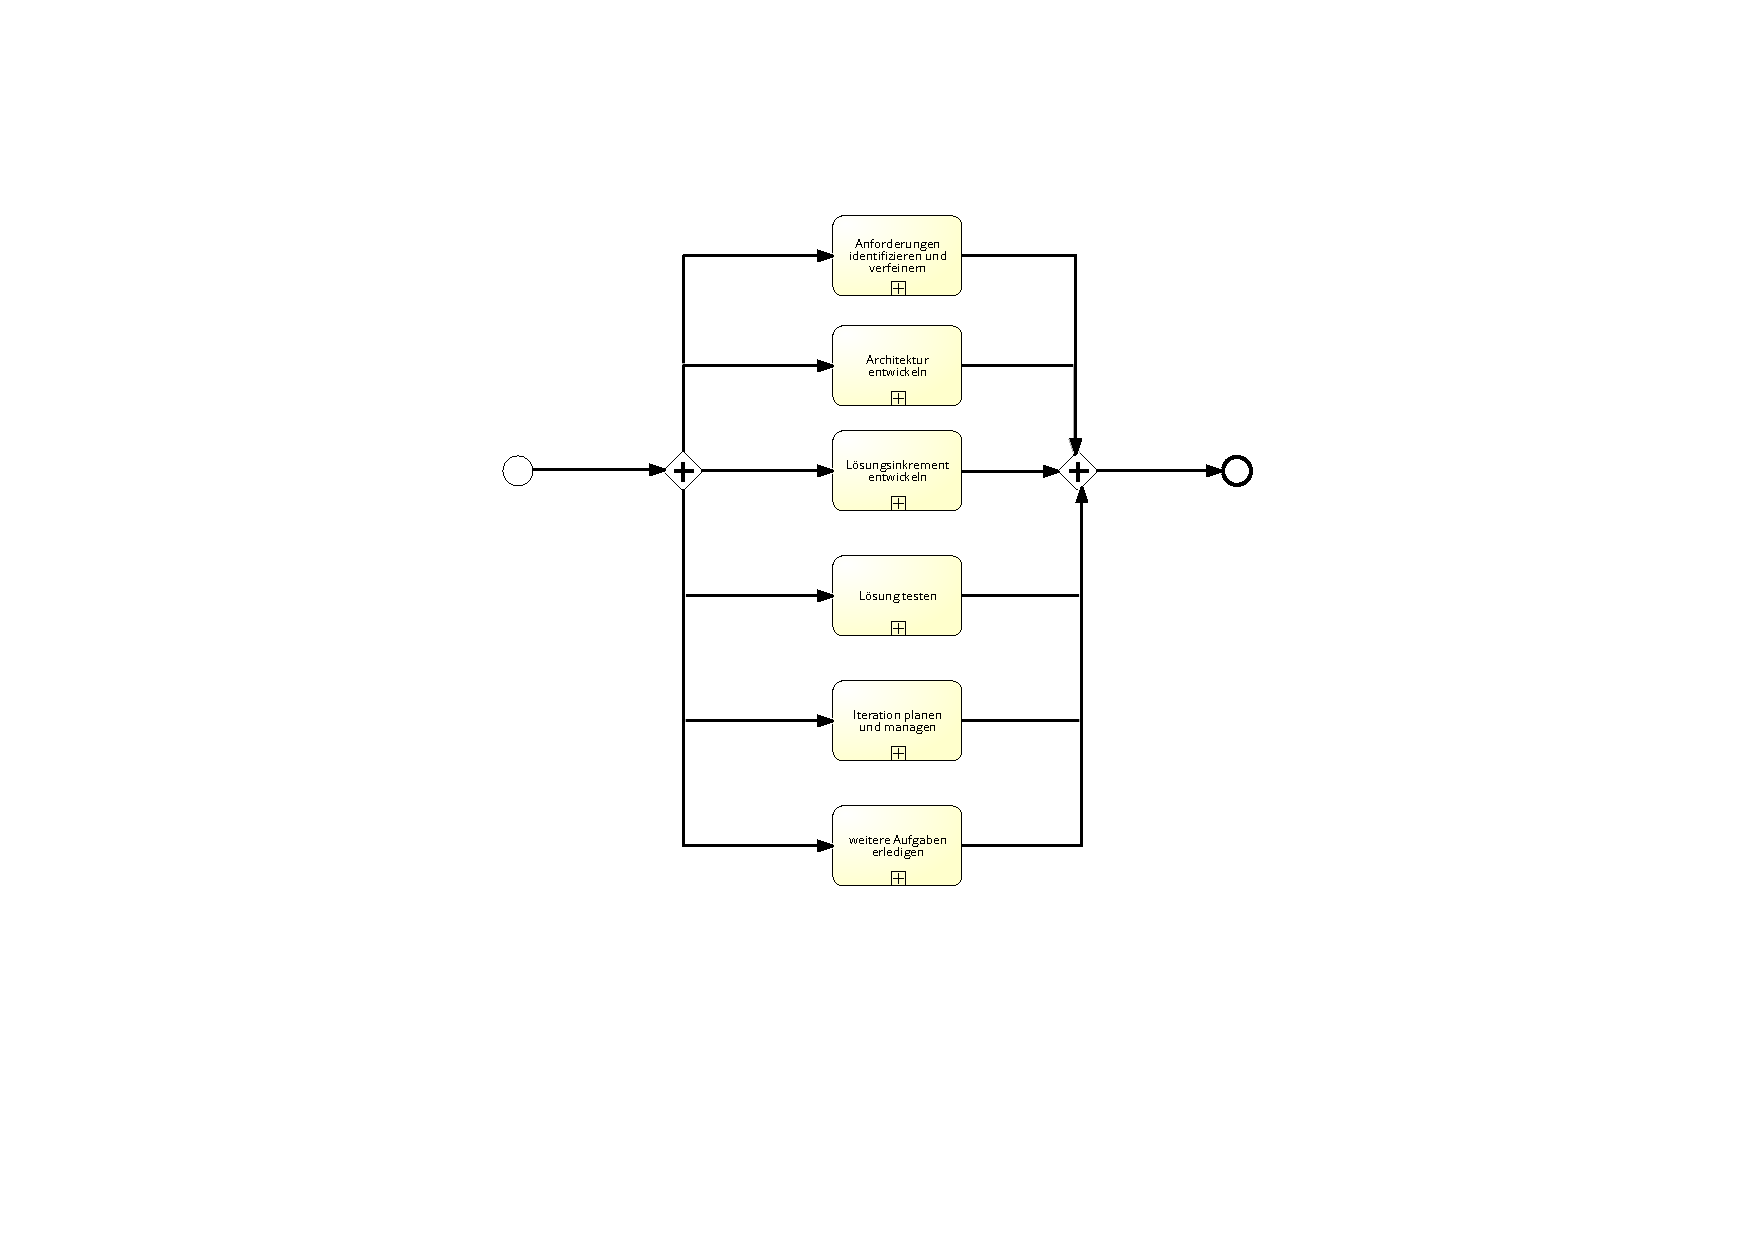
\includegraphics[scale=0.8]{OpenUpElaboration} %pdf, jpg, png...
  \caption{Phasen Open UP Unterprozess Elaboration- imperativ}
  \label{fig:OpenUpElaboration}
\end{center}
\end{figure}

Die imperative Modellierung der Iteration Construction kann Abbildung \ref{fig:OpenUpConstruction} entnommen werden. Hier werden die sechs Aktivitäten \grqq Anforderungen identifizieren und verfeinern\grqq , \grqq Lösungsinkrement entwickeln\grqq , \grqq Lösung testen\grqq , \grqq Iteration planen und managen\grqq , \grqq weitere Aufgaben erledigen\grqq  \ und \grqq Produktdokumentation und Training erstellen\grqq \ nebeneinander parallel ausgeführt.
\begin{figure}[htp]
\begin{center}
  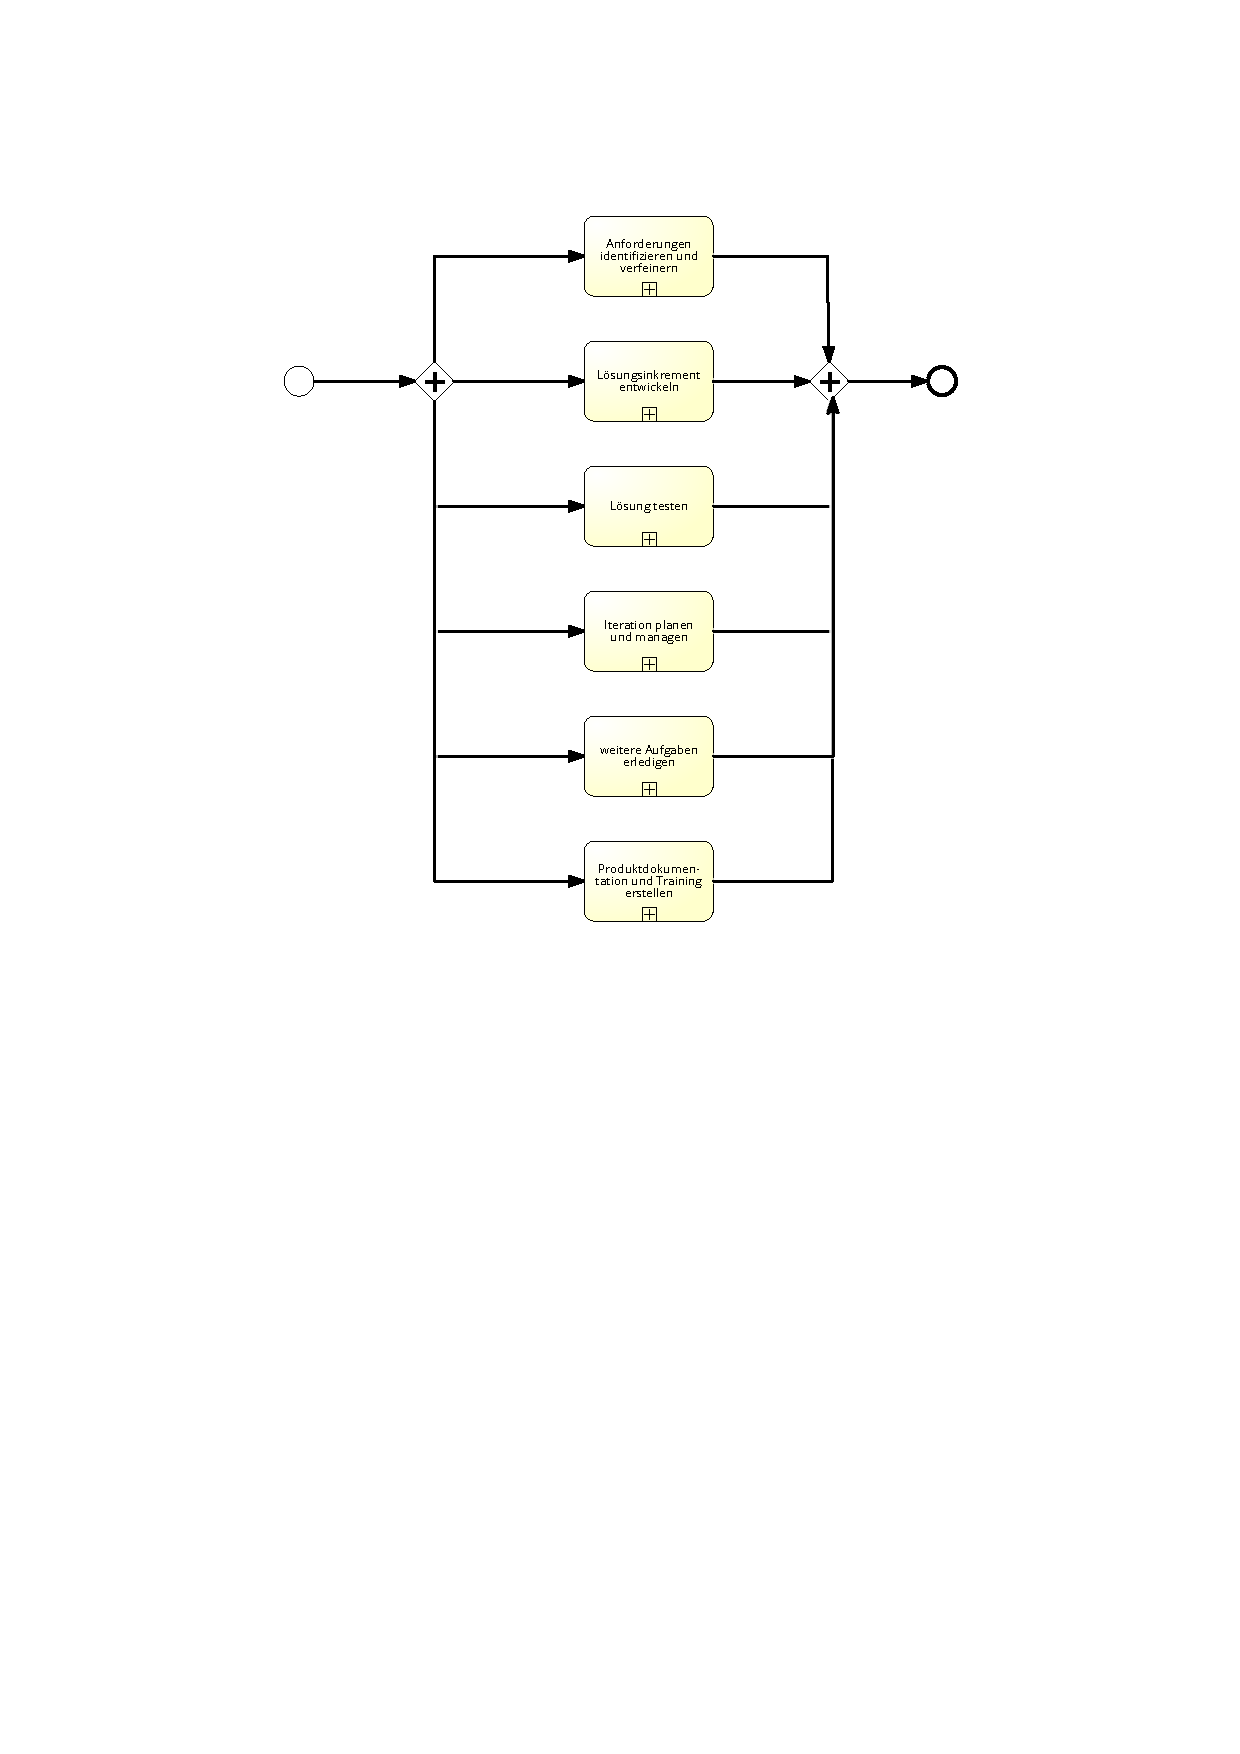
\includegraphics[scale=0.8]{OpenUpConstruction} %pdf, jpg, png...
  \caption{Phasen Open UP Unterprozess Construction- imperativ}
  \label{fig:OpenUpConstruction}
\end{center}
\end{figure}

Abbildung \ref{fig:OpenUpTransition} kann die imperative Modellierung der Iteration Transition entnommen werden. Die Aktivitäten \grqq Release vorbereiten\grqq , \grqq  Produkt Training vorbereiten\grqq, \grqq Lösungsinkrement entwickeln\grqq, \grqq Lösung testen\grqq , \grqq Iteration planen und managen\grqq \ und \grqq weitere Aufgaben erledigen\grqq \ werden parallel zueinander ausgeführt. Nach deren Ausführung können die Aktivitäten Produktdokumentation und Training durchführen \grqq \ sowie \grqq Release deployen\grqq \  parallel zueinander abgearbeitet werden.

\begin{figure}[htp]
\begin{center}
  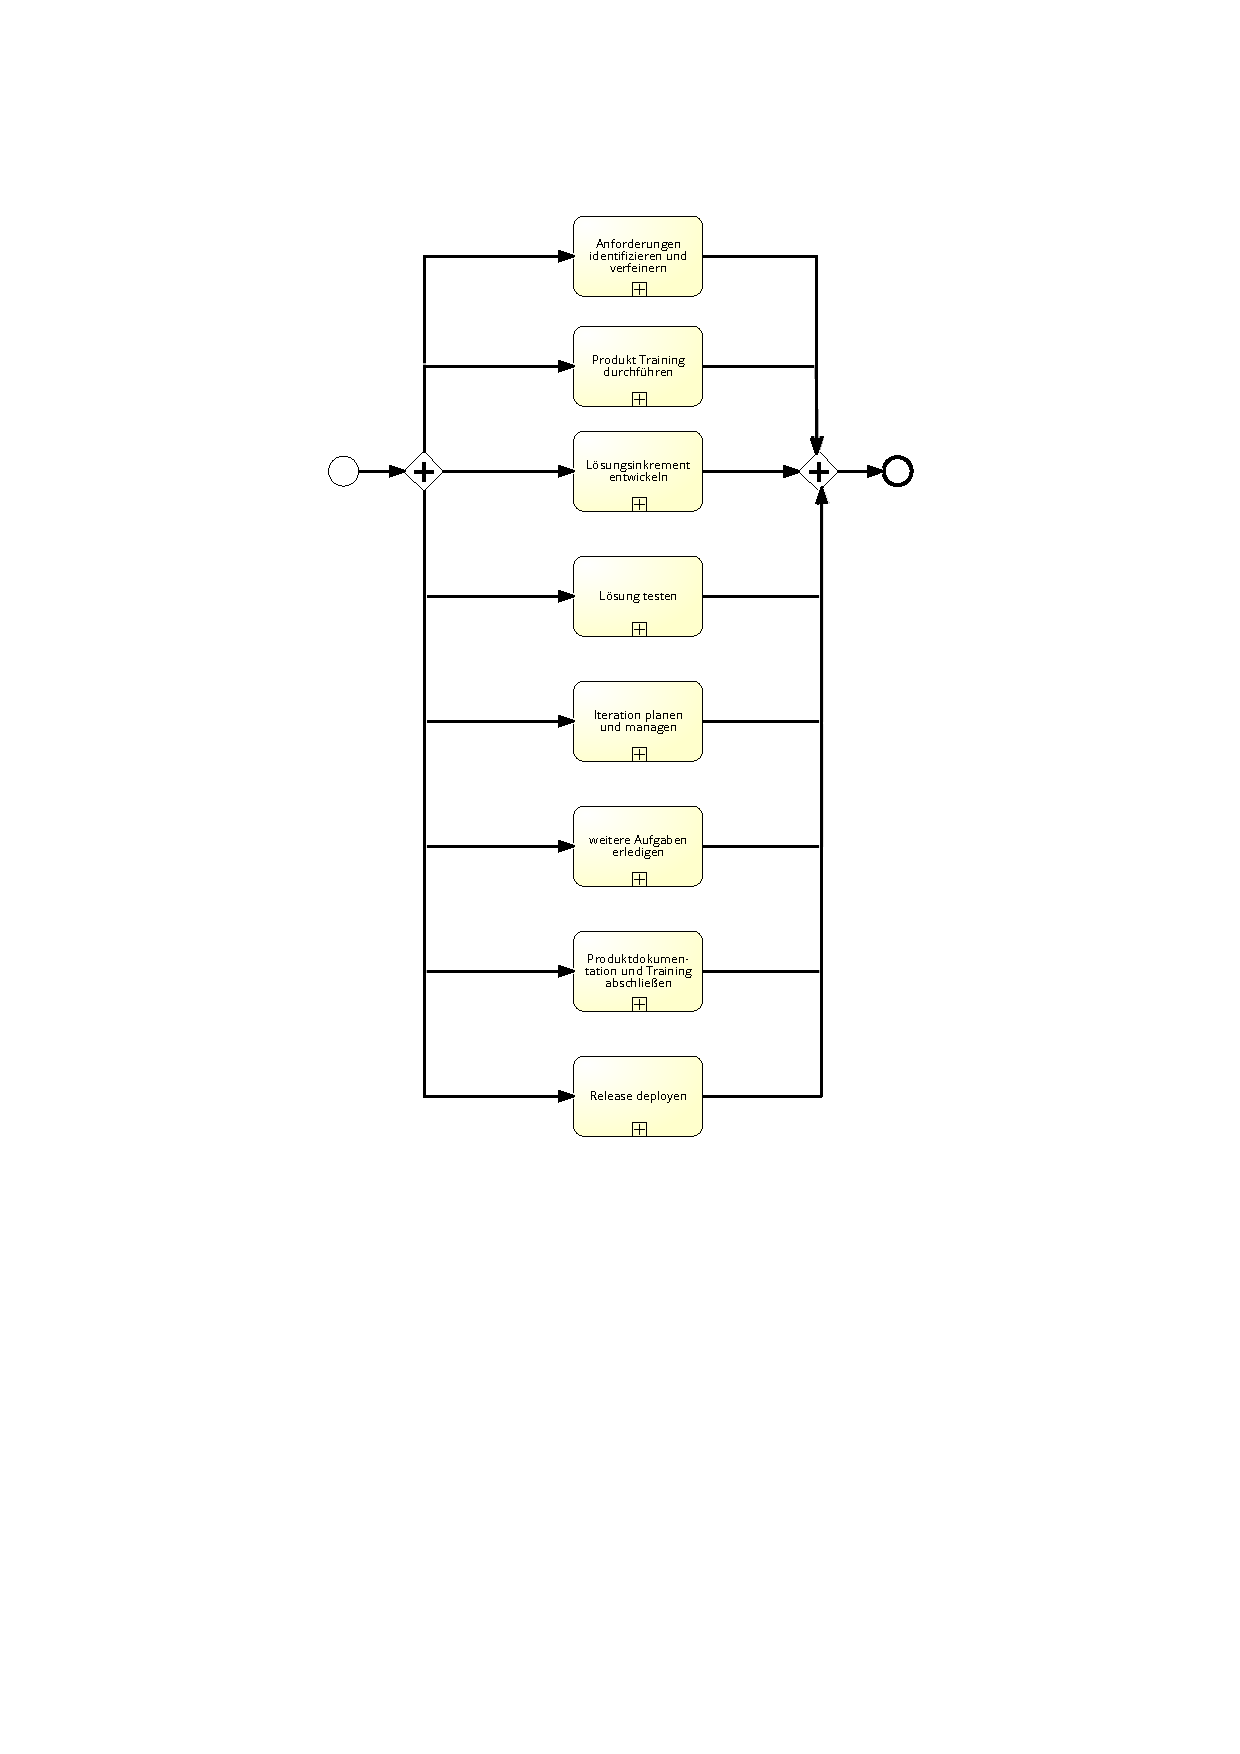
\includegraphics[scale=0.8]{OpenUpTransition} %pdf, jpg, png...
  \caption{Phasen Open UP Unterprozess Transition- imperativ}
  \label{fig:OpenUpTransition}
\end{center}
\end{figure}



Im weiteren Verlauf wird aus jeder der vier Iterationen Inception, Elaboration, Construction und Transition des Open UP jeweils ein repräsentativer Unterprozess modelliert, da die Abbildung aller Unterprozesse aus jeder Itaeration den Rahmen der Arbeit sprengen würde. \newline
Somit wird für die Iteration Inception der Unterprozess \grqq Iteration planen und managen\grqq, für die Iteration Elaboration der Unterprozess \grqq Anforderungen identifizieren und verfeinern, für die Iteration Construction der Unterprozess \grqq Release deployen\grqq \ und für die Iteration Transition der Unterprozess \grqq Produktdokumentation und Training erstellen\grqq \ modelliert. Außerdem wird der in den drei Phasen Elaboration, Construction und Transition wiederkehrende Unterprozess \grqq Lösungsinkrement entwickeln\grqq \ modelliert.

\subsubsection{Lösungsinkrement entwickeln}

Im Unterprozess \textit{Lösungsinkrement entwickeln} geht es um das Design, die Implementierung, das Testen und die Integration der Lösung für eine Anforderung in einem bestimmten Kontext. Sie tritt genauso viele Male auf, wie es Arbeitsaufgaben gibt, die in einer Iteration entwickelt werden müssen.
 Handelt es sich um eine nicht-triviale Veränderung, wird zunächst eine Lösung designt und anschließend ein Entwickeltest implementiert. Bei einer trivialen Änderung an der bestehenden Implementierung kann diese auch direkt in der bestehenden Architektur vorgenommen werden. \newline
 Sobald die Fragen der technischen Umsetzung geklärt sind, werden Entwicklertests implementiert, um die Implementierung zu verifizieren. Anschließend werden diese Entwicklertests ausgeführt.\newline
 Falls bei der Ausführung der Tests Fehler ersichtlich werden, muss eine Lösung für diesen Fehler implementiert werden und die Entwicklertests müssen erneut ausgeführt werden. Dies wird solange wiederholt, bis alle Tests bestanden sind.\newline
An dieser Stelle kann der Entwurf nochmals überdacht werden. Falls hier beschlossen wird, dass der Code überarbeitet werden muss, muss im Prozess zurückgegangen werden und erneut eine Lösung designt werden, da eine Änderung des Codes die Implementation und die Entwicklertests beeinflussen könnte.\newline
 Da es am Besten ist, die Implementierungsteile so klein wie möglich zu halten, sollte zunächst eine kleine Design-Lösung für einen Teil der Arbeitsaufgabe entwickelt werden. Anschließend sollte dies für weitere kleine Teile solange wiederholt werden, bis die gesamte Arbeitsaufgabe implementiert ist. \newline
 In Abbildung \ref{fig:Dev} ist die imperative Modellierung von \grqq Lösungsinkrement entwickeln\grqq \ abgebildet.\newline
 Die Verknüpfung mit dem Exklusiven Gateway am Anfang führt im Falle einer trivialen Änderung zur sofortigen Ausführung der Aktivität \textit{Entwicklertest implementieren}. Falls es sich jedoch um eine typische Änderung handelt, muss zuvor die Aktivität \grqq Lösung designen\grqq \ ausgeführt werden. Im Anschluss an \grqq Entwicklertest implementieren\grqq \ muss die Aktivität \grqq Entwicklertest ausführen\grqq \ durchgeführt werden.\newline
 Hiernach wird im Falle eines fehlgeschlagenen Tests zunächst eine \grqq Lösung implementiert\grqq \ und anschließend erneut der \grqq Entwicklertest ausgeführt\grqq. \newline
 Wenn der Test bestanden ist, muss am Exklusiven Gateway entschieden werden, ob der Code gut designt ist. Falls nein, muss erneut eine Lösung designt werden. Falls doch, kann der Code integriert werden. Ist die Arbeit vollständig erledigt, so ist der Prozess beendet. Wenn jedoch noch weitere Arbeit vorhanden ist, beginnt er von vorne.
 
 
\begin{figure}[htp]
\begin{center}
  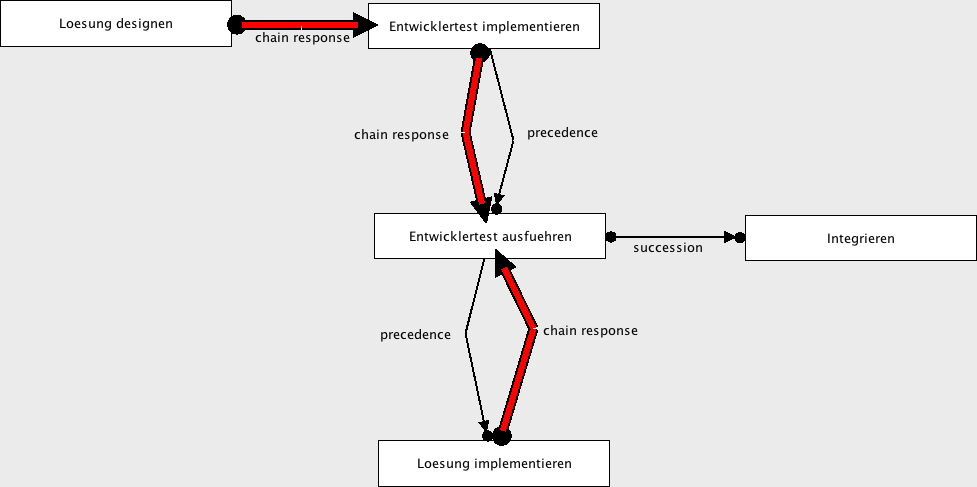
\includegraphics[width=\linewidth]{DevelopSolution} %pdf, jpg, png...
  \caption{Lösungsinkrement entwickeln imperativ}
  \label{fig:Dev}
\end{center}
\end{figure}

\subsubsection{Iteration planen und managen- Inception}

Die Aktivität \grqq Iteration planen und managen\grqq \ wird während des gesamten Projektlebenszyklus ausgeführt. Ihr Ziel ist es, Risiken und Probleme früh genug zu identifizieren, damit diese entschärft werden können, um die Ziele für die Iteration festzulegen und das Team dabei zu unterstützen, diese zu erreichen.
Die Iteration wird durch den Projektmanager und das Team gestartet. Hier findet die Priorisierung der Arbeit für eine gegebene Iteration statt. Der Projektmanager, die Stakeholder und die Teammitglieder einigen sich darauf, was während der Iteration zu entwickeln ist.
Die Teammitglieder melden sich für die Arbeitsaufgaben, die während der Iteration entwickelt werden müssen. Anschließend teilt sich jedes Teammitglied seine Arbeitsaufgaben selbstständig in Arbeitseinheiten ein und schätzt den Aufwand hierfür ab.\newline
Während der Iteration trifft sich das Team regelmäßig, um den aktuellen Stand der Arbeit und eventuelle Probleme zu besprechen. \newline
Abbildung \ref{fig:PlanAndManageIterationInception-2} zeigt die imperative Modellierung von \grqq Iteration planen und managen\grqq. 
Vom Projektmanager sind hierbei nacheinander die Aktivitäten \grqq Iteration planen, Umgebung vorbereiten, Iteration managen\grqq \ und \grqq Ergebnisse festlegen\grqq \ durchzuführen und das Team muss nacheinander die Aktivitäten \grqq Arbeitsaufgaben aussuchen, Arbeitsaufgaben in Entwicklungsaufgaben einteilen\grqq \ sowie \grqq Aufwand abschätzen\grqq \ ausführen. Hierbei gehen jeweils die Artefakte \grqq Arbeitseinheiten-Liste, Iterationsplan\grqq \ und \grqq Risiko-Liste\grqq \ in verschieden Aktivitäten als Input ein und kommen eventuell verändert als Output wieder heraus. \newline
Die Aktivität \grqq Umgebung vorbereiten\grqq \ ist als Unterprozess in Abbildung \ref{fig:Umgebungvorbereiten} dargestellt. Hier müssen vom Projektmanager die Aktivitäten \grqq Prozess Maßschneidern\grqq \ und \grqq Prozess deployen\grqq \ sequentiell erledigt werden, während der Tool Spezialist die Aufgaben \grqq Tools aufsetzen\grqq \ und \grqq Tool-Konfiguration und Implementation verifizieren\grqq \ zu erledigen hat.


\begin{figure}[!htbp]
\begin{center}
  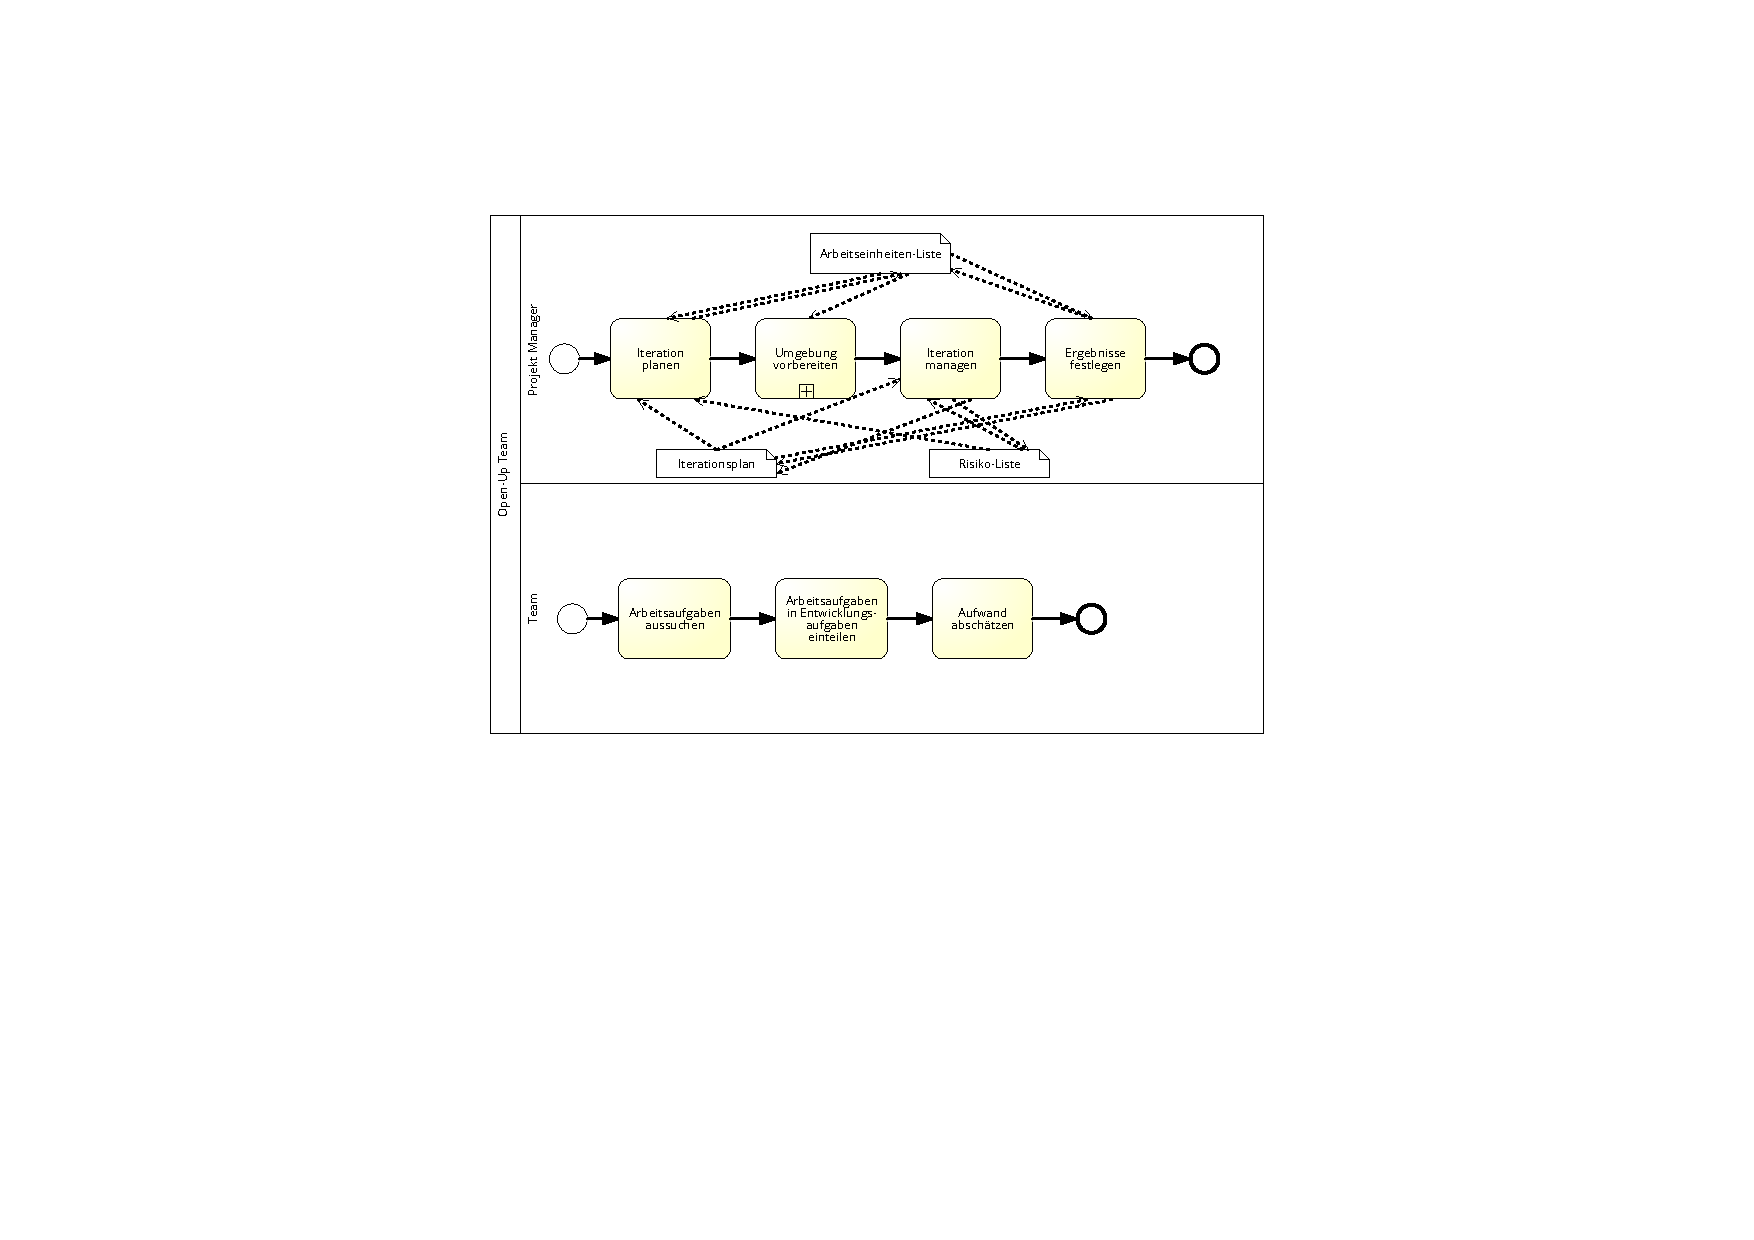
\includegraphics[scale=0.7]{PlanAndManageIterationInception-2} %pdf, jpg, png...
  \caption{Iteration planen und managen imperativ -Inception}
  \label{fig:PlanAndManageIterationInception-2}
\end{center}
\end{figure}

\begin{figure}[!htbp]
\begin{center}
  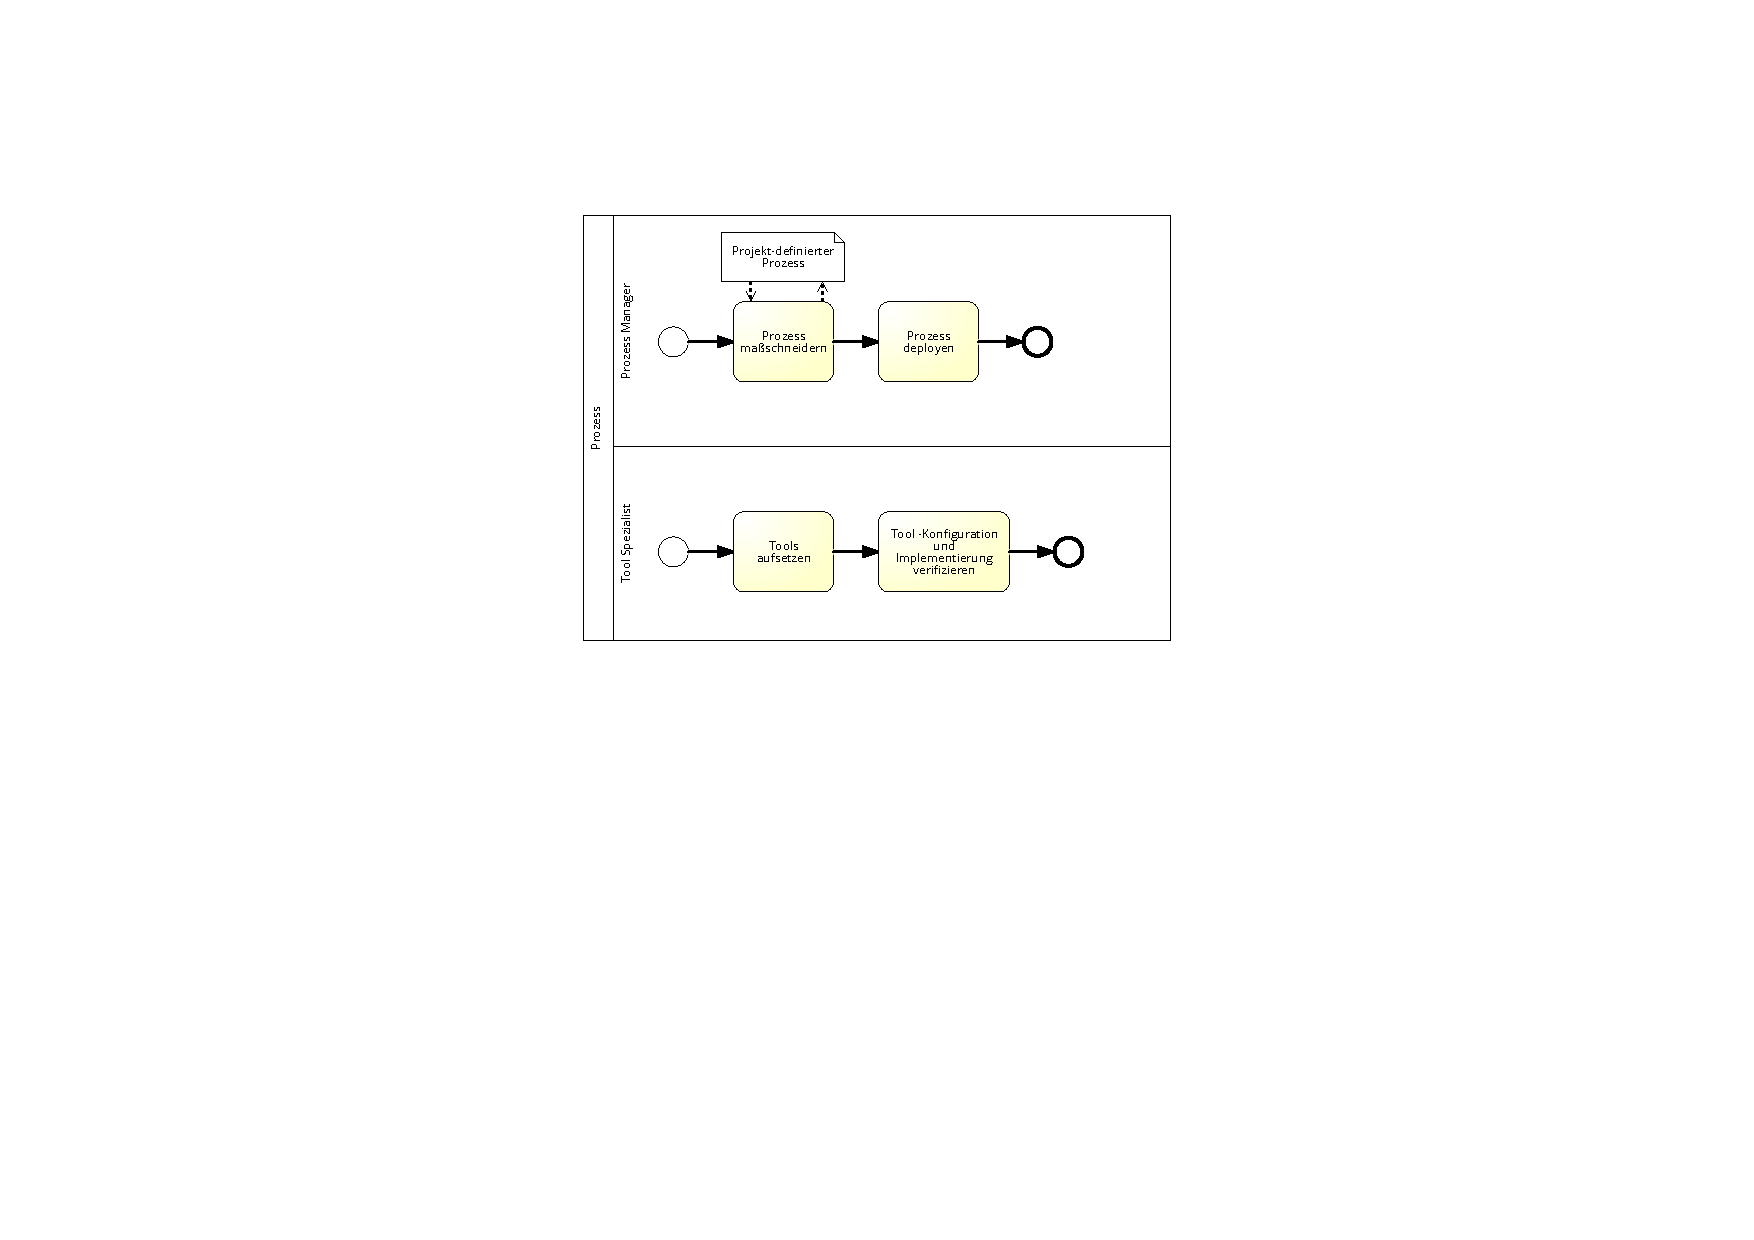
\includegraphics[scale=0.7]{Umgebungvorbereiten} %pdf, jpg, png...
  \caption{Iteration planen und managen imperativ -Inception Unterprozess Umgebung vorbereiten} 
  \label{fig:Umgebungvorbereiten}
\end{center}
\end{figure}

\clearpage


\subsubsection{Anforderungen identifizieren und verfeinern}
 Der Unterprozess \textit{Anforderungen identifizieren und verfeinern} beschreibt die Aufgaben, welche durchzuführen sind, um die Anforderungen eines Systems zu sammeln, zu analysieren und zu validieren bevor die Implementierung und die Validierung stattfinden. Sie wird in Zusammenarbeit mit Stakeholdern und dem gesamten Entwicklungsteam ausgeführt, um sicher zu gehen, dass klare, konsistente, korrekte und nachprüfbare Anforderungen vorhanden sind.\newline
 In der Phase Elaboration liegt der Fokus auf der Definition der Lösung. Hierfür müssen diejenigen Anforderungen gefunden werden, welche für die Stakeholder am wichtigsten sind die besonders herausfordernd oder sogar riskant sind oder eine große Bedeutung für die Architektur haben.\newline
 Dafür ist es notwendig, zunächst die funktionalen und nicht-funktionalen Anforderungen an das System zu erheben. Genau diese Anforderungen stellen dann die Basis für die Kommunikation und die Übereinstimmung zwischen den Stakeholdern und dem Entwicklungsteam dar, in Bezug auf was das System können muss, um die Wünsche der Stakeholder zu erfüllen.\newline
 Weiterhin müssen die Use-Case-Szenarien und die systemweiten Anforderungen ausführlich genug beschrieben werden, um sicher zu gehen, dass die Anforderungen richtig verstanden wurden und dass diese mit den Erwartungen der Stakeholder übereinstimmen.\newline
 Zudem müssen Testfälle und Testdaten für die Anforderungen entwickelt werden, um ein gemeinsames Verständnis für die spezifischen Bedingungen, die die Lösung erfüllen muss, zu erreichen.
 In Abbildung \ref{fig:IdentifyAndOutlineKlein} ist die imperative Modellierung von \grqq Anforderungen identifizieren und verfeinern\grqq \ abgebildet. \newline
 Zunächst muss der Analyst die \grqq Anforderungen identifizieren und abgrenzen\grqq, bevor er anschließend die \grqq Use-Case-Szenarien detaillieren\grqq kann. Daraufhin muss er die \grqq Systemweiten Anforderungen detaillieren\grqq, damit der Tester anschließend die \grqq Testfälle erstellen\grqq kann.\newline
 Hier gehen bei den verschiedenen Aktivitäten die Artefakte \grqq Arbeitseinheitenliste\grqq, \grqq Use Case\grqq, \grqq Glossar\grqq, \grqq Systemweite Anforderungen\grqq, \grqq Use case Modell\grqq, \grqq Technische Spezifikation\grqq \ und \grqq Testfall\grqq \ als Input hinein, bzw. als Output heraus.
 
\begin{figure}[[!htbp]
\begin{center}
  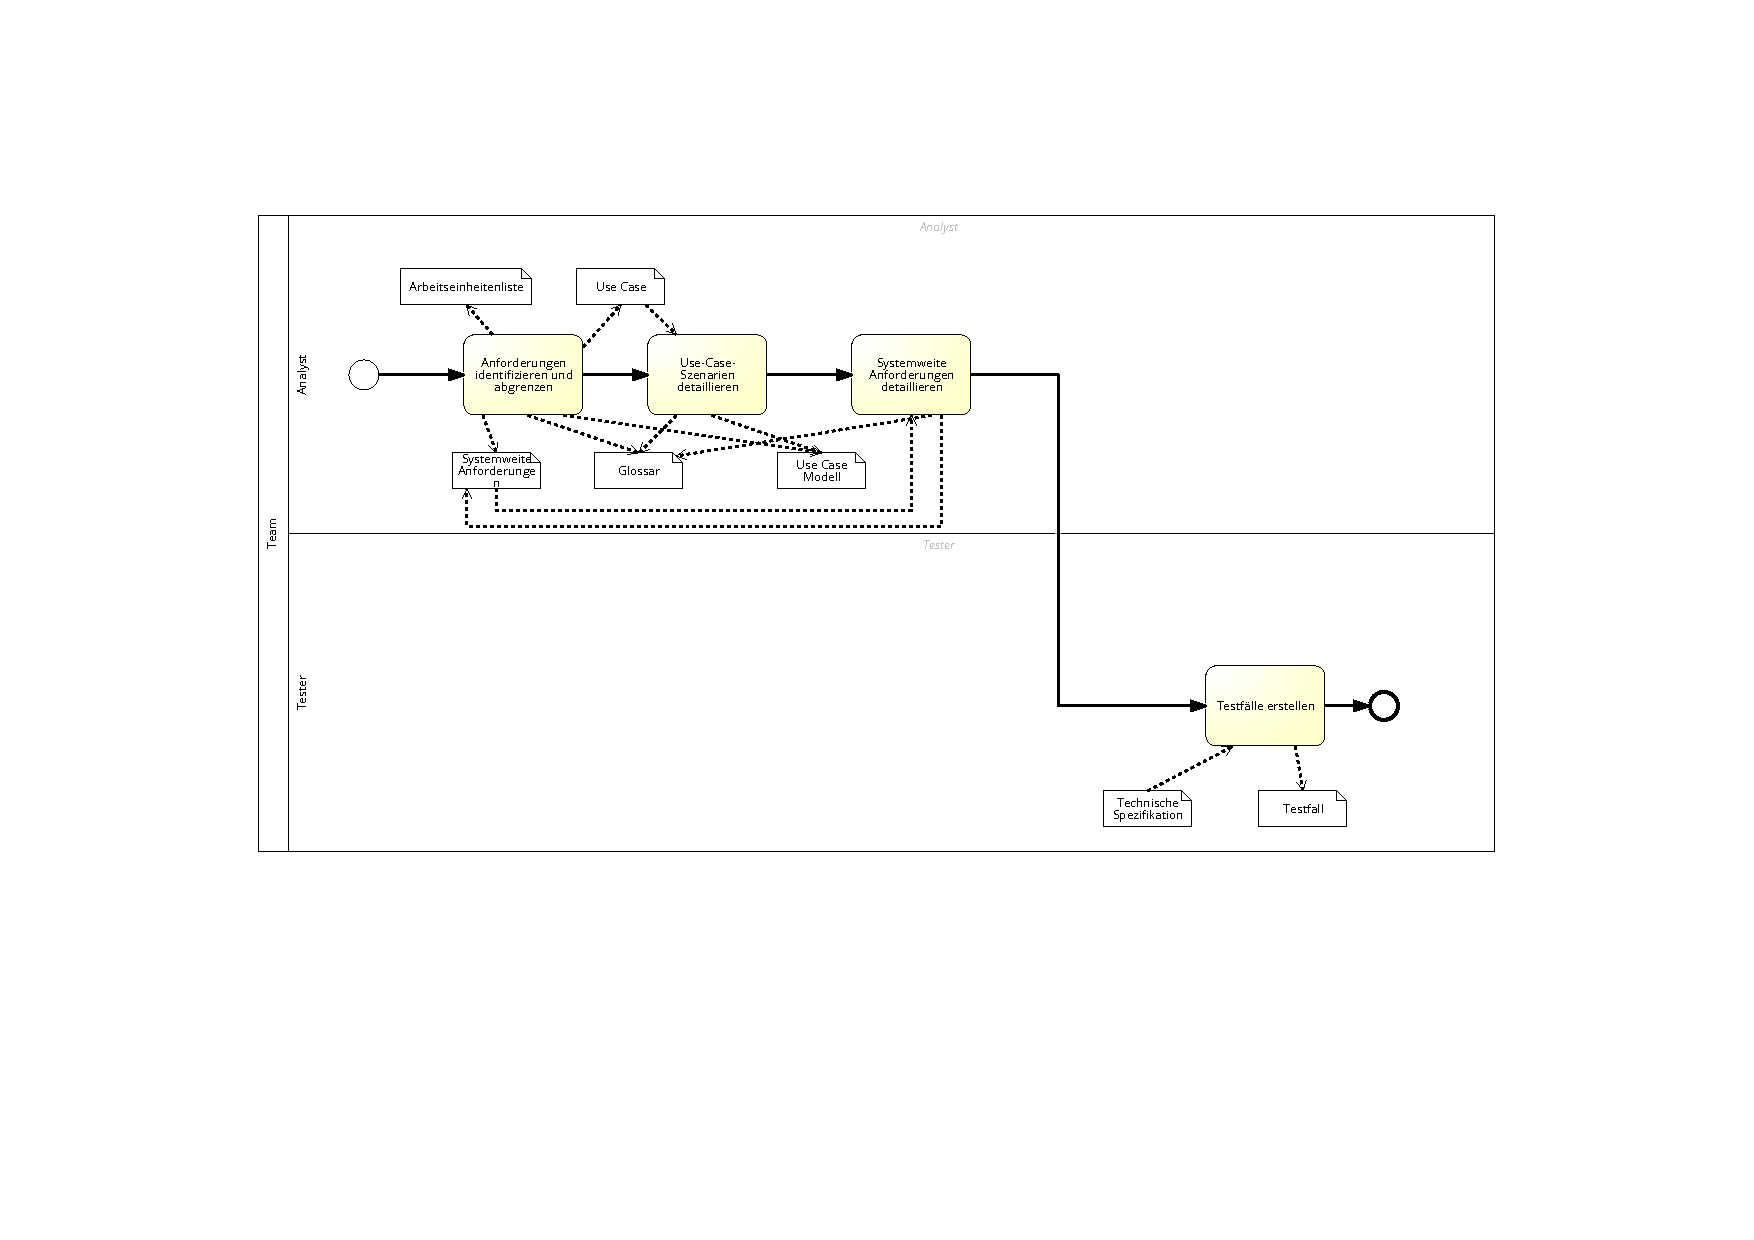
\includegraphics[width=\linewidth]{IdentifyAndOutlineKlein} %pdf, jpg, png...
  \caption{Anforderungen identifizieren und verfeinern-Elaboration}
  \label{fig:IdentifyAndOutlineKlein}
\end{center}
\end{figure}


\subsubsection{Produktdokumentation und Training erstellen-Construction}
 Das Ziel des Unterprozesses \grqq Produktdokumentation und Training erstellen\grqq \ ist es, die Produktdokumentation und Trainingsmaterial vorzubereiten. Da die Produktdokumentation oftmals erst nach Abschluss der Entwicklungstätigkeiten erstellt wird, muss sichergestellt werden, dass die Funktionen die während einer Release entwickelt werden klar dokumentiert werden, solange die Funktionalität noch frisch in den Köpfen der Teammitglieder vorhanden ist.\newline
 Hierfür ist es notwendig, dass genug Informationen über die Funktionen, die in einer bestimmten Release entwickelt wurden, dokumentiert werden, um dem Kunden während der gesamten Lebenszeit des Produkts nützlich zu sein.\newline
 Weiterhin müssen den Endnutzern hilfreiche Informationen bereit gestellt werden in Form von Benutzerhandbüchern, Tutorials, häufig gestellte Fragen (FAQs), Online-Hilfedateien, Installationsanweisungen und Betriebsabläufe. 
 Zudem muss sichergestellt werden, dass diejenigen, die mit der Unterstützung des Systems beauftragt sind, genug Informationen über das Produkt haben, um ihre Arbeit effektiv durchzuführen, nachdem das Produkt produktiv gegangen ist. Außerdem muss die Einführung des Produkts ermöglicht werden und dessen ordnungsgemäße Verwendung gewährleistet werden.\newline
 
 Die imperative Modellierung von \grqq Produktdokumentation und Training erstellen\grqq \ kann Abbildung \ref{fig:DevelopProductDocumentationKlein} entnommen werden.
 Hier sind vom technischen Schreiber nacheinander die Aktivitäten \grqq Produktdokumentation erstellen\grqq, \grqq Benutzerdokumentation erstellen\grqq, \grqq Unterstützungsdokumentation erstellen\grqq \ und \grqq Trainingsmaterial erstellen\grqq \ auszuführen. Aus den jeweiligen Aktivitäten entstehen sodann die Artefakte \grqq Produktdokumentation, Benutzerdokumentation, Unterstützungsdokumentation\grqq \ und \grqq Trainingsmaterial\grqq.
 
\begin{figure}[!htbp]
\begin{center}
  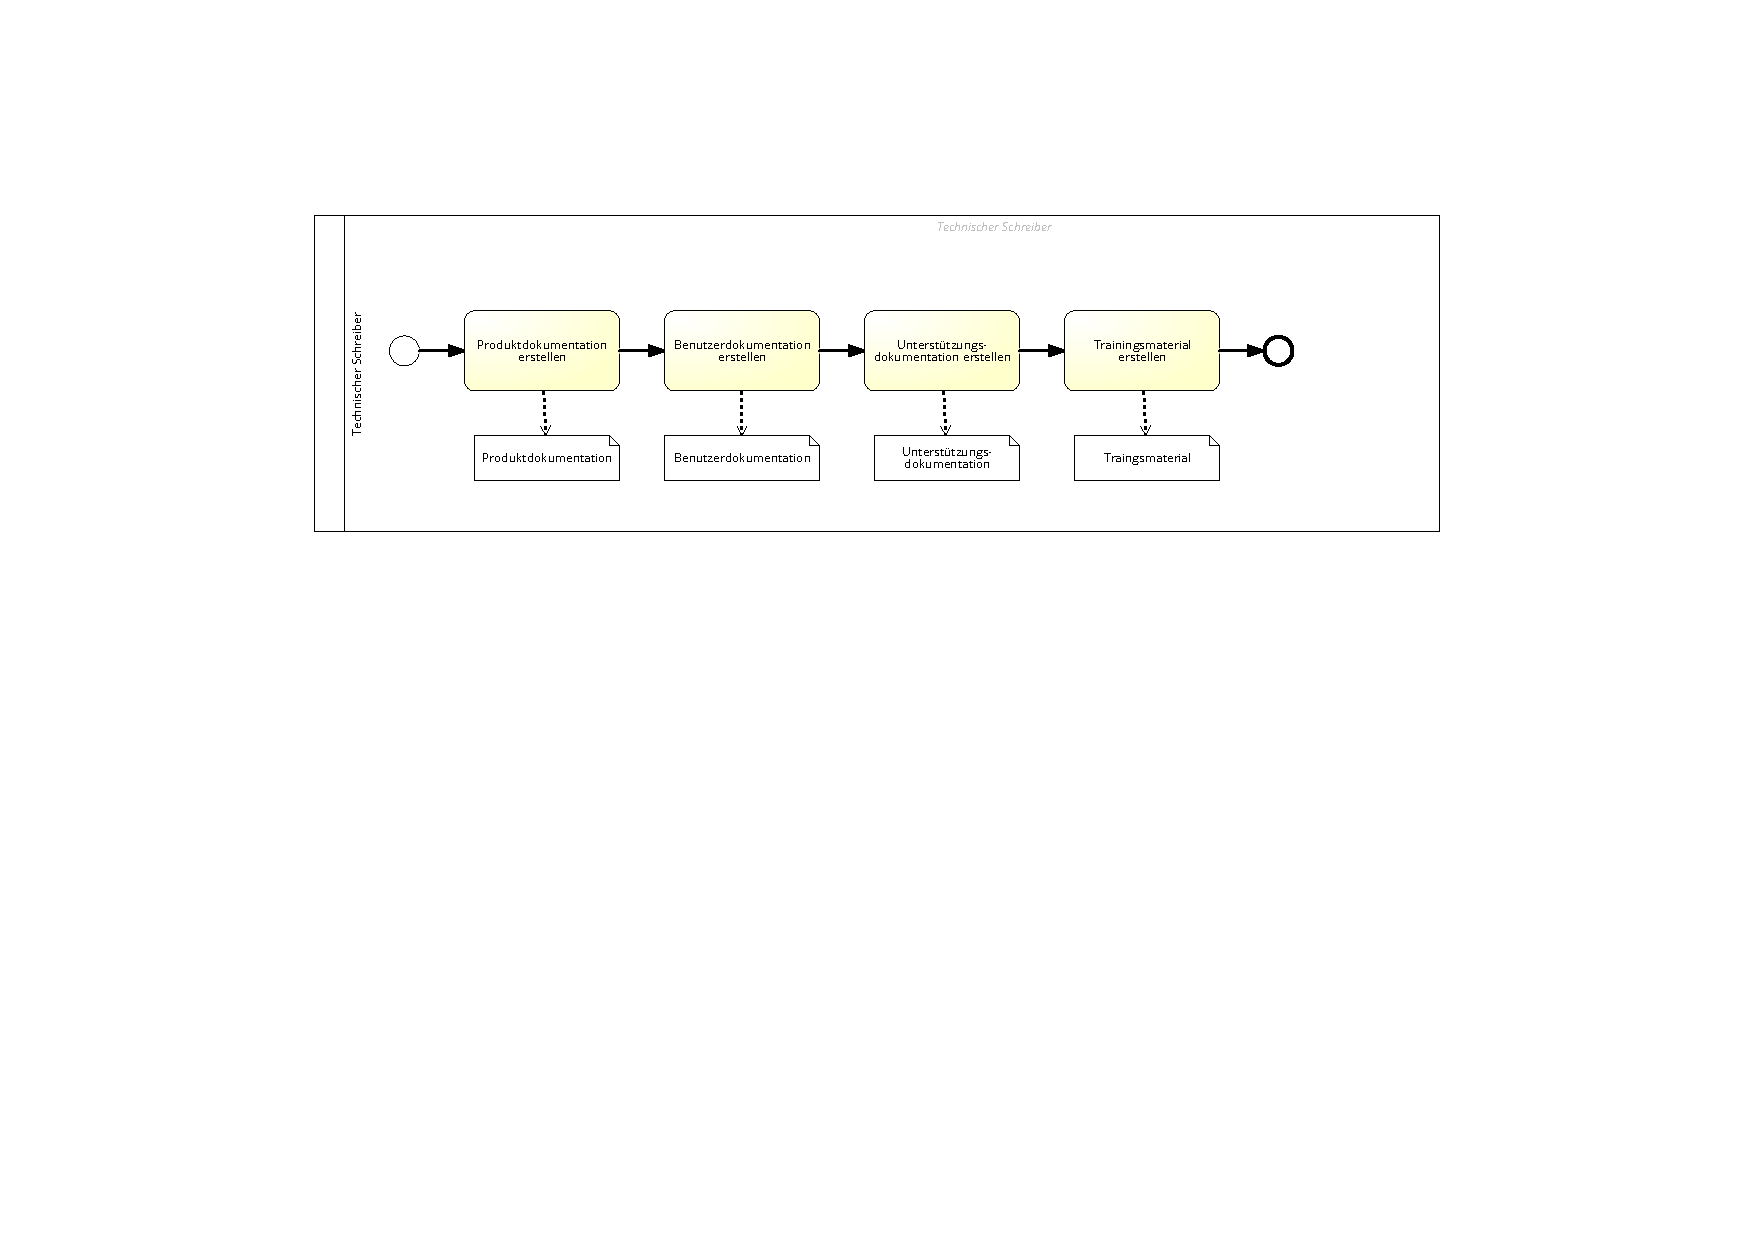
\includegraphics[width=\linewidth]{DevelopProductDocumentationKlein} %pdf, jpg, png...
  \caption{Produktdokumentation und Training erstellen - Construction}
  \label{fig:DevelopProductDocumentationKlein}
\end{center}
\end{figure}


\subsubsection{Release deployen-Transition}


Das Ergebnis dieses Unterprozesses ist die Release eines Sets von integrierten Komponenten in der Integrationsumgebung. Hierfür ist es notwendig, ein komplettes, bereitstellungsfähiges Paket zu erstellen, welches vom Deployment Engineer in die Bereitstellungsumgebung releast werden kann.
 Außerdem muss sichergestellt werden, dass der Roll-Out aus klaren, geprüften und wiederholbaren Anweisungen besteht und das Risiko eines Bereitstellungsfehlers muss minimiert werden.
 Zudem muss sichergestellt werden, dass eine Release zu keinen ungewollten Unterbrechungen im Ablauf in der Produktionsumgebung führt. Falls eine Release Probleme verursacht oder sie von den Stakeholdern als untauglich empfunden wird, muss diese Release von der Produktionsumgebung so schnell wie möglich entfernt werden. Zusätzlich muss dafür gesorgt werden, dass Informationen über eine anstehende Release weitest möglich verteilt werden.\newline
 
  Abbildung \ref{fig:DeployReleaseTransitionKlein} zeigt die imperative Modellierung von\grqq Release deployen\grqq.
  Somit muss der Entwickler zunächst die \grqq Release zusammenstellen\grqq, bevor der Deployment Engineer nacheinander die Aktivitäten \grqq Deploymentplan ausführen\grqq \ und \grqq erfolgreiches Deployment sicherstellen\grqq \ ausführt. Falls das Deployment erfolgreich ist, wird gleich anschließend die Aktivität \grqq Releasemitteilungen übermitteln\grqq \ ausgeführt. Ist das Deployment nicht erfolgreich, muss zunächst die Aktivität \grqq Backoutplan ausführen\grqq \ erledigt werden und erst danach die Aktivität \grqq Releasemitteilungen übermitteln\grqq \ ausgeführt werden.


\begin{figure}[!htbp]
\begin{center}
  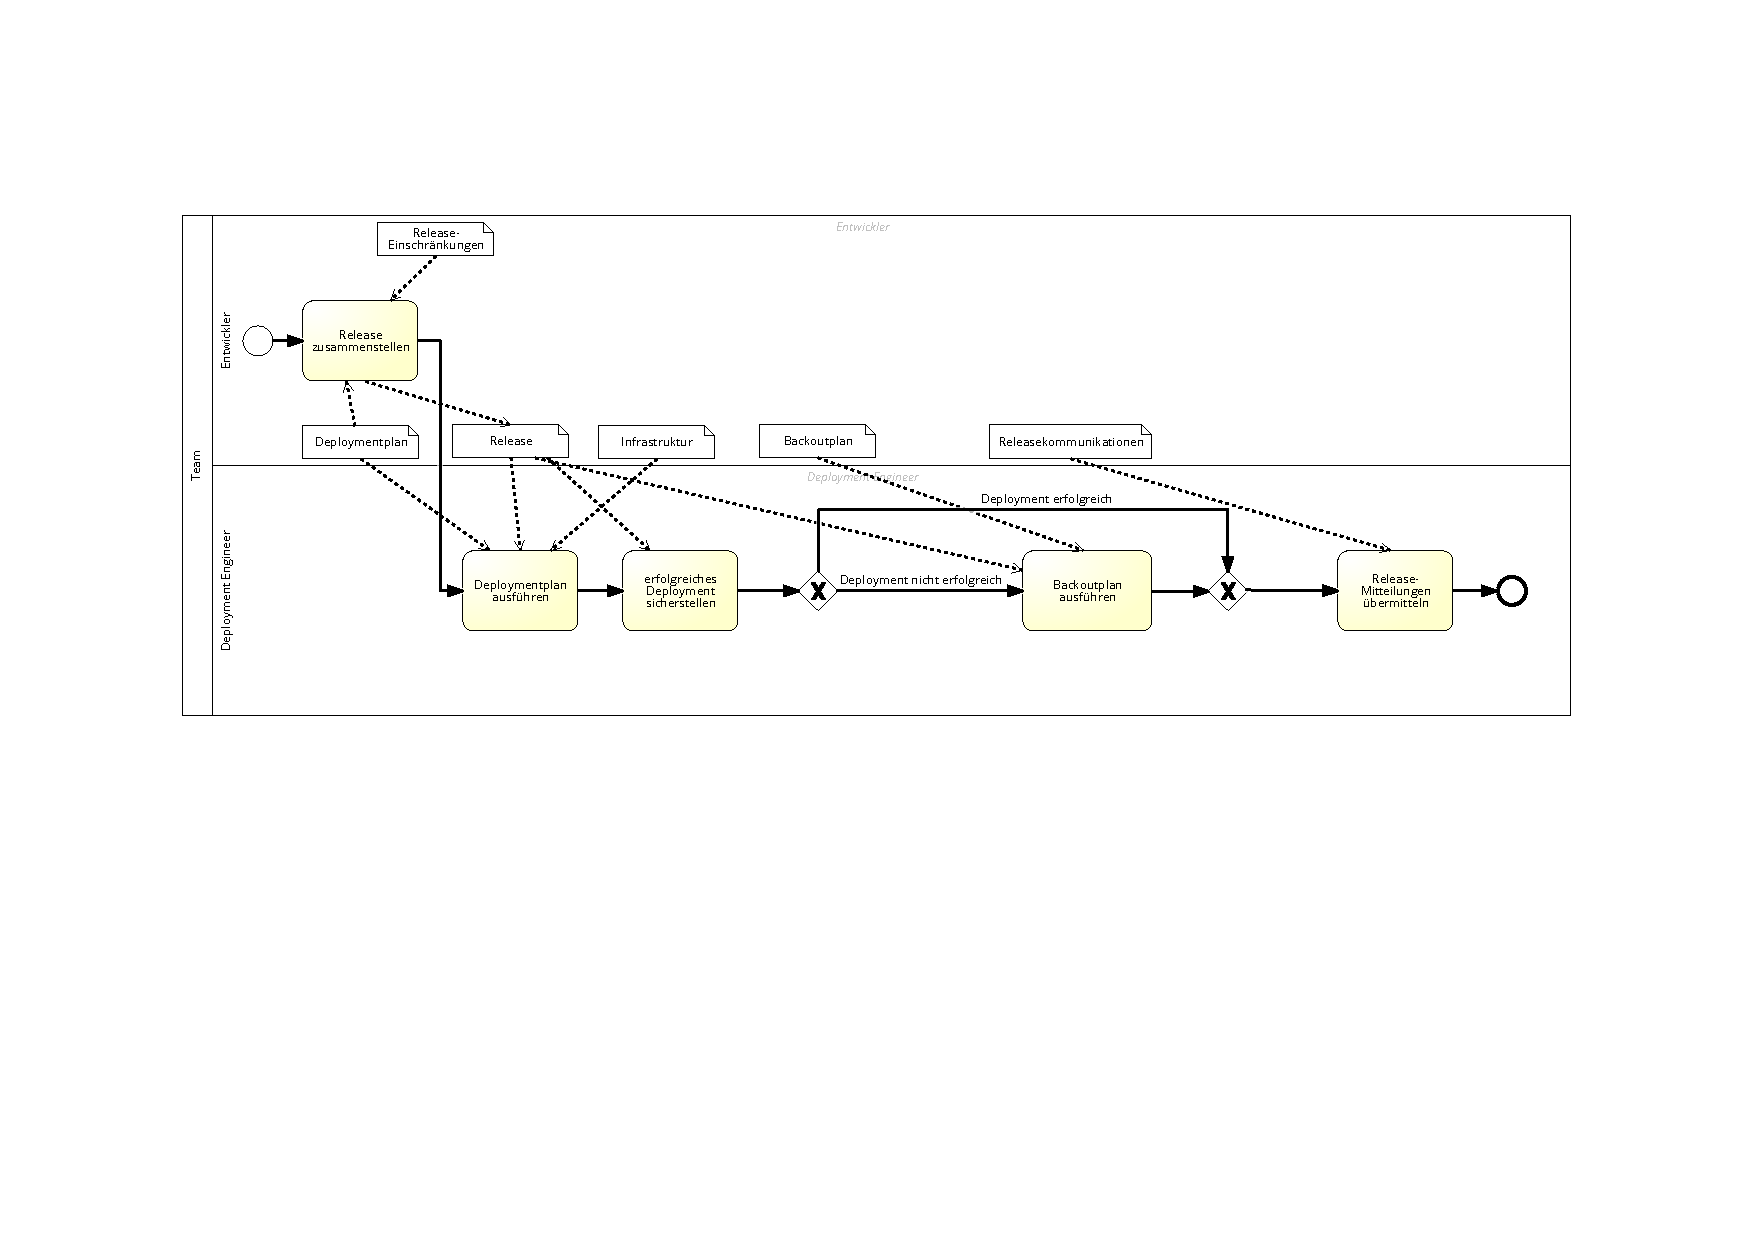
\includegraphics[width=\linewidth]{DeployReleaseTransitionKlein} %pdf, jpg, png...
  \caption{Release deployen-Transition}
  \label{fig:DeployReleaseTransitionKlein}
\end{center}
\end{figure}



\clearpage

\subsection{Deklarative Modellierung Open UP}

Im folgenden wird die entsprechende deklarative Modellierung der Prozesse durchgeführt.

\subsubsection{Phasen des Open UP}


In Abbildung \ref{fig:OpenUpPhasenDec} sind die vier Phasen des Open UP deklarativ modelliert. Jede Phase kann in Iterationen mehrmals durchlaufen werden. Aus diesem Grund sind die vier Phasen durch das Constraint \textit{succesion} miteinander verbunden. Hierdurch wird gewährleistet, dass jede Phase so oft ausgeführt werden kann, wie nötig, aber dass ebenfalls die Reihenfolge eingehalten wird. So kann z.B. die Phase Elaboration erst durchlaufen werden, nachdem die Phase Inception durchlaufen wurde.
\begin{figure}[htp]
\begin{center}
  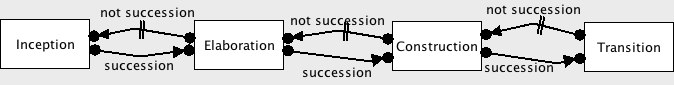
\includegraphics[width=\linewidth]{OpenUpPhasenDec} %pdf, jpg, png...
  \caption{Phasen Open UP- deklarativ}
  \label{fig:OpenUpPhasenDec}
\end{center}
\end{figure}




Abbildung \ref{fig:InceptionDecUnter} zeigt die deklarative Modellierung der Iteration Inception. Die Aktivität \textit{Projekt planen und managen} kann parallel zu allen anderen Aktivitäten des Modells ausgeführt werden.\newline
Nach Ausführung der Aktivität \grqq Iteration planen\grqq \ werden die Aktivitäten \grqq Anforderungen identifizieren und aufbereiten\grqq \ und \grqq auf technisches Vorgehen einigen\grqq \ parallel zueinander ausgeführt. Aus diesem Grund sind die Aktivitäten \grqq Anforderungen identifizieren und aufbereiten\grqq \ und \grqq auf technisches Vorgehen einigen\grqq \ mit der Aktivität \grqq Projekt planen und managen\grqq \ durch das Constraint \textit{succession} verbunden, da sie erst nach deren Ausführung ausgeführt werden dürfen und auch ausgeführt werden müssen. \newline

\begin{figure}[htp]
\begin{center}
  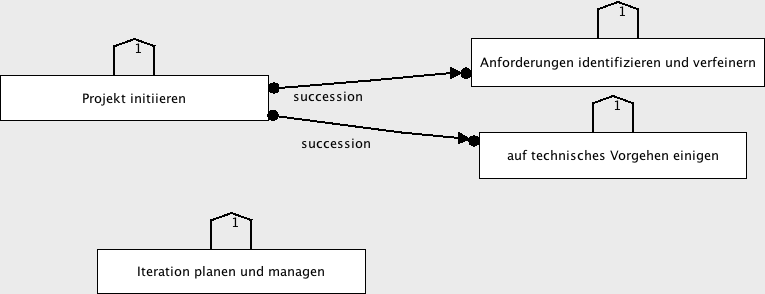
\includegraphics[width=\linewidth]{InceptionDecUnter} %pdf, jpg, png...
  \caption{Phasen Open UP Unterprozess Inception- deklarativ}
  \label{fig:InceptionDecUnter}
\end{center}
\end{figure}

In Abbildung \ref{fig:ElaborationDecUnter} ist die deklarative Modellierung der Iteration Elaboration abgebildet. Die sechs Aktivtäten\grqq Anforderungen identifizieren und verfeinern, Architektur entwickeln, Lösungsinkrement entwickeln, Lösung testen, Iteration planen und managen\grqq \ sowie \grqq weitere Aufgaben erledigen\grqq \ werden parallel zueinander ausgeführt. Aus diesem Grund befindet sich lediglich das Constraint \textit{Ecactly 1} an jeder Aktivität, da sie innerhalb einer Prozessinstanz nur einmal ausgeführt werden dürfen, dies aber in beliebiger Reihenfolge. Im Falle einer weiteren Iteration der Phase Elaboration wird eine neue Prozessinstanz aufgerufen. \newline

\begin{figure}[htp]
\begin{center}
  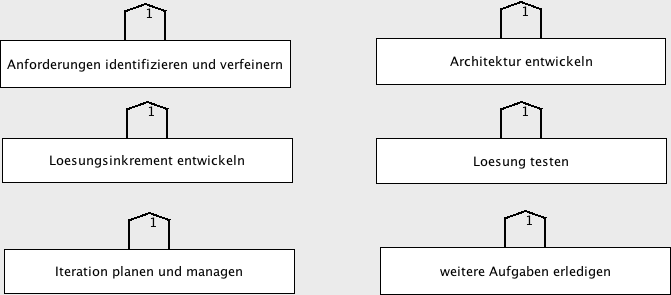
\includegraphics[width=\linewidth]{ElaborationDecUnter} %pdf, jpg, png...
  \caption{Phasen Open UP Unterprozess Elaboration- deklarativ} 
  \label{fig:ElaborationDecUnter}
\end{center}
\end{figure}

Die deklarative Modellierung der Iteration Construction kann Abbildung \ref{fig:ConstructionDecUnter} entnommen werden. Hier werden die sechs Aktivitäten \textit{Anforderungen identifizieren und verfeinern, Lösungsinkrement entwickeln, Lösung testen, Iteration planen und managen, weitere Aufgaben erledigen} und \textit{Produktdokumentation und Training erstellen} nebeneinander parallel ausgeführt.
\begin{figure}[htp]
\begin{center}
  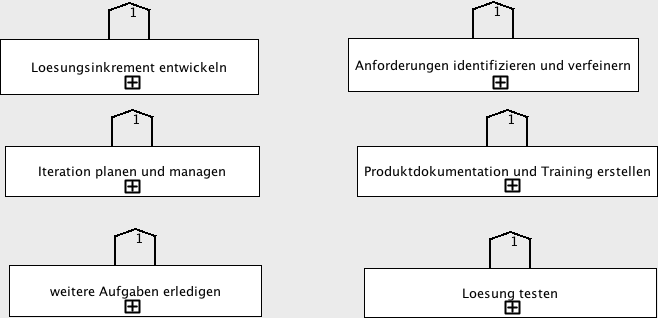
\includegraphics[width=\linewidth]{ConstructionDecUnter} %pdf, jpg, png...
  \caption{Phasen Open UP Unterprozess Construction- deklarativ}
  \label{fig:ConstructionDecUnter}
\end{center}
\end{figure}

In \ref{fig:TransitionDecUnter} ist die deklarative Modellierung der Iteration Transition abgebildet.\newline
Die Aktivitäten \grqq Release vorbereiten, Produkt Training vorbereiten, Lösungsinkrement entwickeln, Lösung testen, Iteration planen und managen, weitere Aufgaben erledigen\grqq \ werden parallel zueinander bearbeitet. Produkt Training durchfuehren sowie \grqq Release für die Produktion freigeben\grqq \  können anschließen parallel zueinander ausgeführt werden. Daher befindet sich zwischen diesen beiden Aktivitäten und allen anderen Aktivitäten das Constraint \textit{precedence}.

\begin{figure}[htp]
\begin{center}
  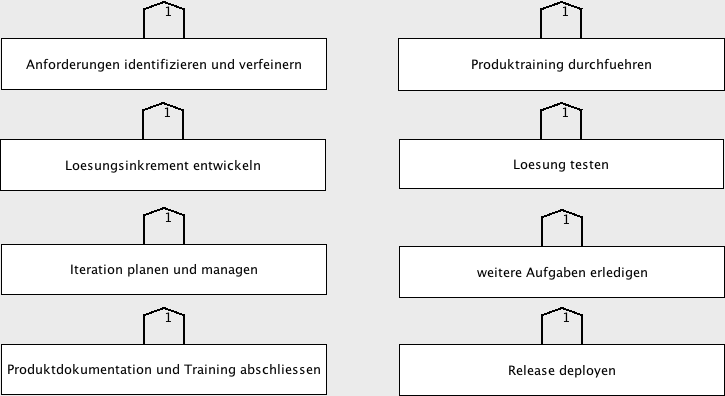
\includegraphics[width=\linewidth]{TransitionDecUnter} %pdf, jpg, png...
  \caption{Phasen Open UP Unterprozess Transition- deklarativ}
  \label{fig:TransitionDecUnter}
\end{center}
\end{figure}



Im weiteren Verlauf wird aus jeder der vier Iterationen Inception, Elaboration, Construction und Transition des Open UP jeweils ein Unterprozess modelliert, da die Abbildung aller Unterprozesse aus jeder Phase den Rahmen der Arbeit sprengen würde. \newline
Somit wird für die Iteration Inception der Unterprozess \textit{Iteration planen und managen}, für die Itertion Elaboration der Unterprozess \textit{Anforderungen identifizieren und verfeinern}, für die Iteration Construction der Unterprozess \textit{Release deployen} und für die Iteration Transition der Unterprozess \textit{Produktdokumentation und Training erstellen} modelliert. Außerdem wird der in den drei Iterationen Elaboration, Construction und Transition wiederkehrende Unterprozess \textit{Lösungsinkrement entwickeln} modelliert.


Die deklarative Modellierung von Lösungsinkrement entwickeln kann Abbildung \ref{fig:Develop} entnommen werden.\newline
Falls eine \grqq Lösung designt\grqq \ wird, muss danach der \grqq Entwicklertest implementiert\grqq \ werden. Dies ist durch das Constraint \textit{chain response} zwischen diesen beiden Aktivitäten verlangt. Wenn der Entwicklertest implementiert wird, muss er danach auch ausgeführt werden und er kann nur ausgeführt werden, falls er vorher implementiert wurde (Constraints \textit{chain response} und \textit{precedence}).\newline
Bevor die Lösung implementiert werden kann, muss vorher der Entwicklertest ausgeführt werden (Constraint \textit{precedence}) und nach der Implementierung der Lösung muss nochmals der Entwicklertest ausgeführt werden (Constraint chain response).\newline
Vor dem \grqq Integrieren\grqq \ muss der Entwicklertest ausgeführt worden sein, was durch das Constraint \textit{precedence} vorgegeben wird.
\begin{figure}[htp]
\begin{center}
  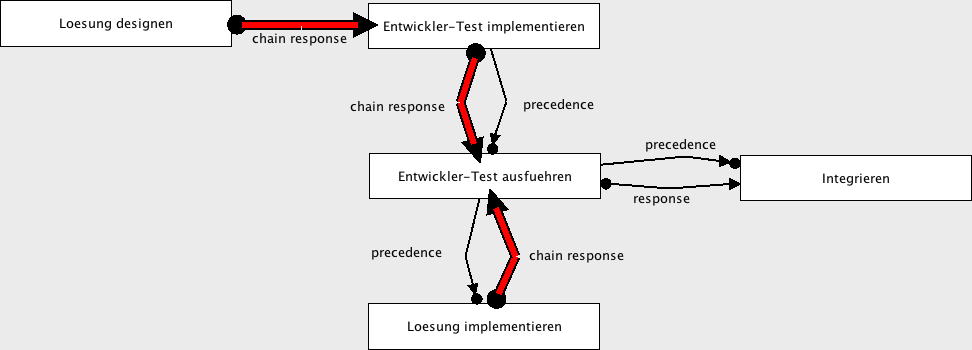
\includegraphics[width=\linewidth]{DevelopSolutionIncrement} %pdf, jpg, png...
  \caption{Lösungsinkrement entwickeln- deklarativ}
  \label{fig:Develop}
\end{center}
\end{figure}

Die deklarative Modellierung von Iteration planen und managen findet sich in den Abbildungen \ref{fig:IterationPlanenDec} und \ref{fig:UmgebungVorbereitenDec}. Gestartet werden kann mit den Aktivitäten \grqq Iteration planen\grqq \ oder \grqq Arbeitsaufgaben aussuchen\grqq, da diese unabhängig voneinander und von zwei verschiedenen Personen ausgeführt werden können.\newline
Danach können entweder die Aktivitäten \grqq Umgebung vorbereiten\grqq \ oder \grqq Arbeitsaufgaben in Entwicklungsaufgaben einteilen\grqq \ ausgeführt werden. Diese sind jeweils mit ihrer Vorgängeraktivität durch das Constraint \textit{succession} verbunden und müssen deshalb auf die Ausführung ihres Vorgängers warten und nach dessen Ausführung bearbeitet werden.\newline
Das gleiche Ausführungsverhalten gilt auch für die anderen Aktivitäten im Prozess. 



\begin{figure}[htp]
\begin{center}
  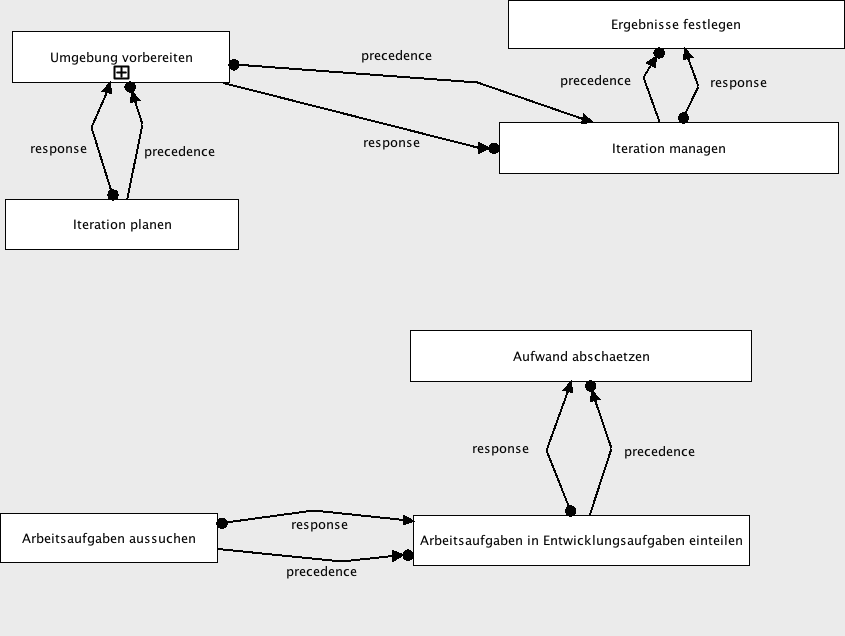
\includegraphics[width=\linewidth]{IterationPlanenDec} %pdf, jpg, png...
  \caption{Iteration planen und managen-Inception deklarativ}
  \label{fig:IterationPlanenDec}
\end{center}
\end{figure}

\begin{figure}[htp]
\begin{center}
  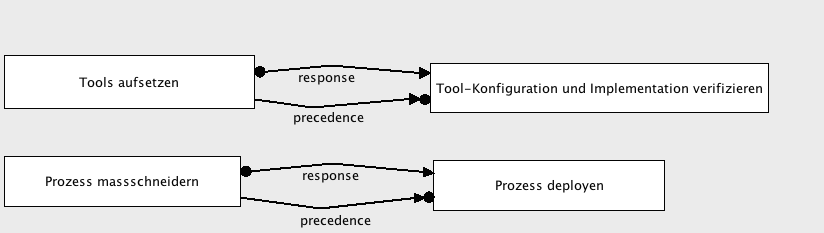
\includegraphics[width=\linewidth]{UmgebungvorbereitenDec} %pdf, jpg, png...
  \caption{Iteration planen und managen- Inception Unterprozess Umgebung vorbereiten- deklarativ}
  \label{fig:UmgebungVorbereitenDec}
\end{center}
\end{figure}


In Abbildung \ref{fig:IdentifyAndRefineDecKlein} ist die deklarative Modellierung von Anforderungen identifizieren und verfeinern dargestellt.\newline
Zu Beginn muss die Aktivität \grqq Anforderungen identifizieren und abgrenzen\grqq \ ausgeführt werden, was durch das init-Label dargestellt ist. Im Anschluss muss die Aktivität \grqq Use-Case-Szenarien detaillieren\grqq \ ausgeführt werden. Dies ist durch das Constraint \textit{chain response} festgelegt. Das Constraint \textit{precedence} legt hingegen fest, dass bevor \grqq Use-Case-Szenarien detaillieren\grqq \ ausgeführt werden kann, zunächst \grqq Anforderungen identifizieren und abgrenzen\grqq \ bearbeitet werden muss. Die gleichen Constraints gelten zwischen \grqq Use-Case-Szenarien detaillieren\grqq \ und \grqq Systemweite Anforderungen detaillieren\grqq \ sowie zwischen \grqq Systemweite Anforderungen detaillieren\grqq \ und \grqq Testfaelle erstellen\grqq. Alle Aktivitäten werden genau einmal ausgeführt, was jeweils durch das 1-Label dargestellt ist. 

\begin{figure}[h]
\begin{center}
  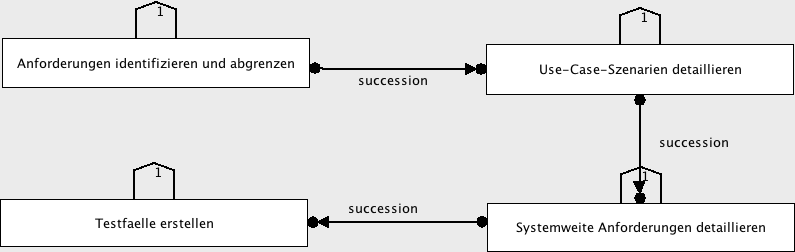
\includegraphics[width=\linewidth]{IdentifyAndRefineDecKlein} %pdf, jpg, png...
  \caption{Anforderungen identifizieren und verfeinern-Elaboration}
  \label{fig:IdentifyAndRefineDecKlein}
\end{center}
\end{figure}



Abbildung \ref{fig:DevelopProductDecKlein} zeigt die deklarative Modellierung von Produktdokumentation und Training erstellen.
Zu Beginn muss die Aktivität \grqq Produktdokumentation entwickeln\grqq \ ausgeführt werden, was durch das init-Label dargestellt ist. Im Anschluss muss die Aktivität \grqq Benutzerdokumentation entwickeln\grqq \ bearbeitet werden. Dies ist durch das Constraint \textit{chain response} festgelegt. Das Constraint \textit{precedence} legt hingegen fest, dass bevor \grqq Benutzerdokumentation entwickeln\grqq \ ausgeführt werden kann, zunächst \grqq Produktdokumentation entwickeln\grqq \ bearbeitet werden muss. Die gleichen Constraints gelten zwischen \grqq Benutzerdokumentation entwickeln\grqq \ und \grqq Unterstützungsdokumentation entwickeln\grqq \ sowie zwischen \grqq Unterstützungsdokumentation entwickeln\grqq \ und \grqq Trainingsmaterial entwickeln\grqq. Alle Aktivitäten werden genau einmal ausgeführt, was jeweils durch das 1-Label beschriebenist. 

\begin{figure}[htp]
\begin{center}
  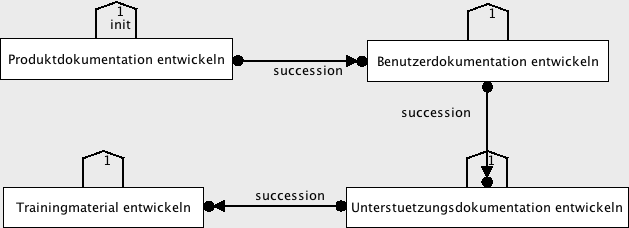
\includegraphics[scale=0.6]{DevelopProductDecKlein} %pdf, jpg, png...
  \caption{Produktdokumentation und Training erstellen-Construction}
  \label{fig:DevelopProductDecKlein}
\end{center}
\end{figure}

Abbildung \ref{fig:DeployReleaseDecKlein} zeigt die deklarative Modellierung von Deploy Release.\newline
Zu Beginn muss Die Aktivität\grqq Release zusammenstellen\grqq \ bearbeitet werden, was durch das init-Constraint vorgegeben ist. Danach wird muss die Aktivität \textit{Deploymentplan ausfuehren} durchgeführt werden (Constraint response), aber erst nachdem \grqq Release zusammenstellen\grqq \ durchgeführt wurde (Contsraint precedence).\newline
Die gleichen Constraints gelten zwischen den Aktivitäten \grqq Deploymentplan ausfuehren\grqq \ und \grqq erfolgreiches Deployment sicherstellen\grqq.\newline
Nach Abschluss der Aktivität \grqq erfolgreiches Deployment sicherstellen\grqq \ kann entweder die Aktivität \grqq Backoutplan ausfuehren\grqq \ ausgeführt werden, welche optinal ist (0..1 Constraint) oder die Aktivität \textit{Release-Mitteilungen uebermitteln}, welche auf jeden Fall ausgeführt werden muss.\newline 
Nach Ausführung von \grqq Release-Mitteilungen uebermitteln\grqq \ darf \grqq Backoutplan ausfuehren\grqq \ nicht mehr durchgeführt werden. Dies stellt das Constraint \textit{not succession} sicher.
\begin{figure}[htp]
\begin{center}
  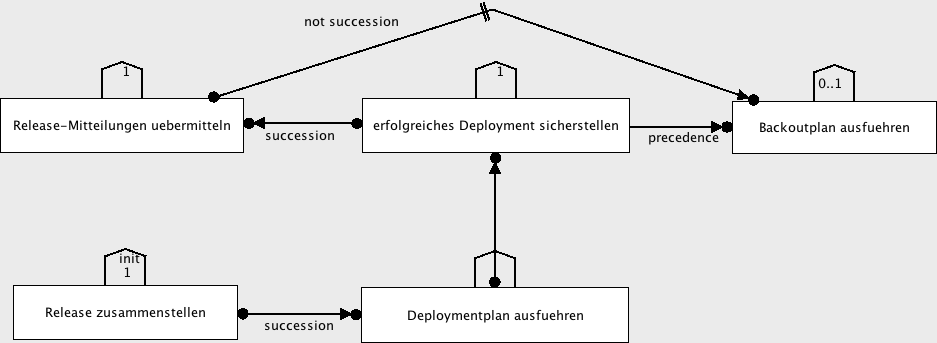
\includegraphics[width=\linewidth]{DeployReleaseDecKlein} %pdf, jpg, png...
  \caption{Release deployen-Transition}
  \label{fig:DeployReleaseDecKlein}
\end{center}
\end{figure}

\clearpage

\subsection{Vergleich}

Nachfolgend wird der vergleich der erstellten Modelle für den Open UP anhand der in Kapitel 4 definierten Anforderungen durchgeführt.

\subsubsection {Phasen Open UP}


Abbildung \ref{fig:PhasenOpenUpExcel} zeigt die Auswertung der Elemente im Modell \grqq Phasen des Open UP\grqq. Während bei BPMN vier Aktivitäten, acht Gateways (keine unterschiedlichen) und 17 Sequenzflusselemente, also gesamt 29 Elemente für das Modell benötigt werden, werden in ConDec nur vier Aktivitäten und sechs Constraints (zwei verschiedene), also insgesamt zehn Elemente verwendet.

\begin{figure}[htp]
\begin{center}
  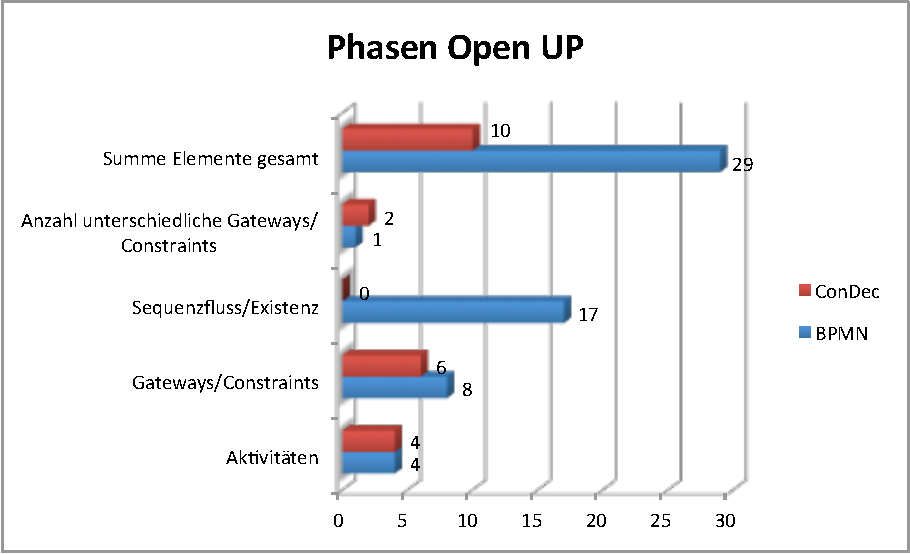
\includegraphics[scale=0.6]{PhasenOpenUpExcel} %pdf, jpg, png...
  \caption{Phasen Open UP}
  \label{fig:PhasenOpenUpExcel}
\end{center}
\end{figure}



\subsubsection {Iterationen Open UP-Inception}

Die Anzahl der Elemente zur Darstellung der Iterationen \grqq Inception\grqq, \grqq Elaboration\grqq, \grqq Construction\grqq \ und \grqq Transition\grqq \ in ConDec und BPMN können Abbildung \ref{fig:PhasenExcel} entnommen werden. BPMN benötigt somit insgesamt 19 Elemente zur Darstellung der Iteration Inception (vier Aktivitäten, vier Gateways und 15 Verbindungselemente), ConDec nur zehn (vier Aktivitäten, sechs Constraints). Bei BPMN wird nur eine Sorte an Gateways verwendet und bei ConDec werden zwei unterschiedliche Constraints benötigt.\newline
\begin{figure}[htp]
\begin{center}
  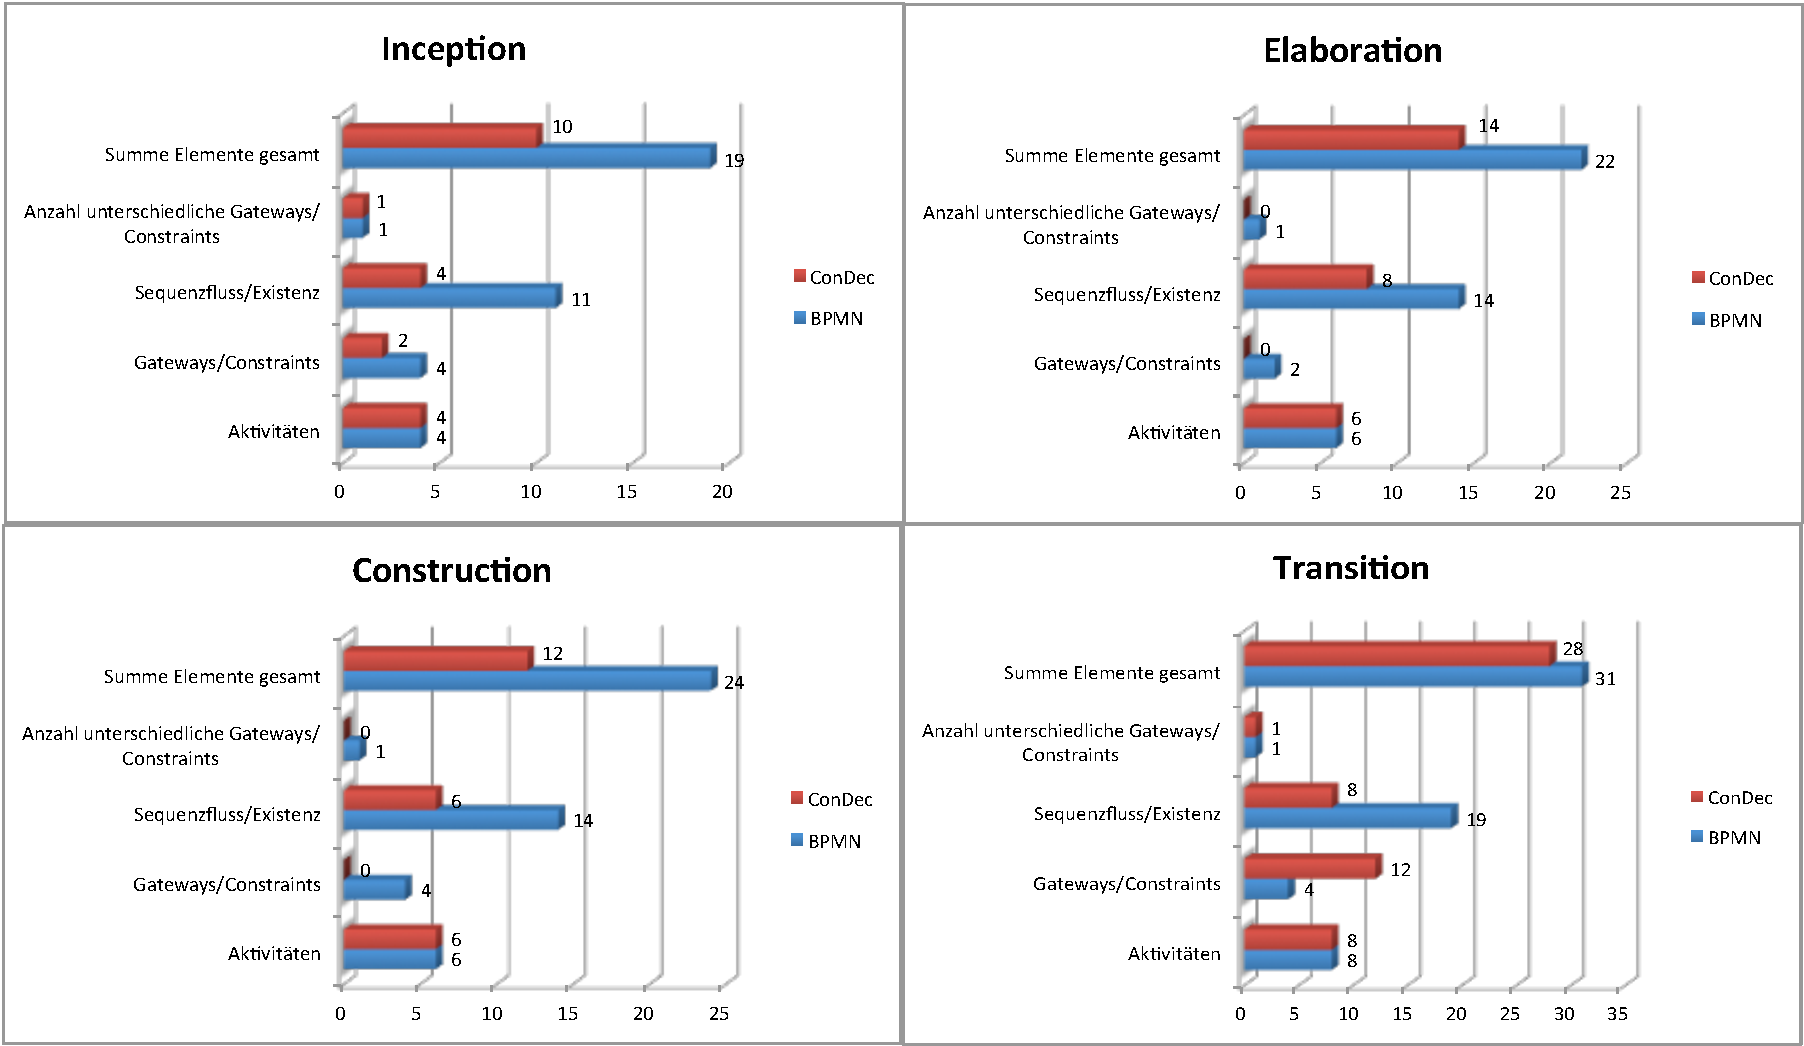
\includegraphics[width=\textwidth]{PhasenExcel} %pdf, jpg, png...
  \caption{Open UP-Inception}
  \label{fig:PhasenExcel}
\end{center}
\end{figure}

Zur Darstellung der Iteration \grqq Elaboration\grqq \ bedarf es in BPMN insgesamt 22 Elementen und in ConDec 14 Elementen wie Abbildung \ref{fig:PhasenExcel} entnommen werden kann. Weiterhin werden jeweils sechs Aktivitäten in beiden Prozessmodellierungssprachen verwendet. In BPMN sind zwei Gateways (keine unterschiedlichen) und 14 Sequenzflusselemente, also insgesamt 16 Verbindungselemente notwendig. ConDec hingegen braucht acht Existenz-Constraints. \newline

Abbildung \ref{fig:PhasenExcel} kann die Anzahl der Elemente zur Darstellung der Iteration \grqq Construction\grqq \ entnommen werden. Demnach benötigt es in BPMN 24 Elemente und in ConDec 12 Elemente zur Darstellung des Prozesses. Sowohl in BPMN, als auch in ConDec werden jeweils sechs Aktivitäten benötigt. In BPMN sind vier Gateways (keine unterschiedlichen) und 14 Sequenzflusselemente erforderlich. In ConDec werden sechs Existenz-Constraints zur Darstellung des Ablaufes verwendet.\newline


Die Anzahl der notwendigen Elemente zur Darstellung der Iteration \grqq Transition\grqq \ kann Abbildung \ref{fig:PhasenExcel} entnommen werden. Somit bedarf es jeweils acht Aktivitäten. BPMN benötigt vier Gateways (keine unterschiedlichen) und 19 Sequenzflusselemente zur korrekten Modellierung. In ConDec braucht es insgesamt acht Existenz-Constraints und 12 Constraints zur Darstellung des Ablaufes.\newline


In Abbildung \ref{fig:LoesungsinkrementExcel} ist die Anzahl der Elemente zur Darstellung des Prozesses \grqq Lösungsinkrement entwickeln\grqq \ abgebildet. Es werden sowohl in BPMN, als auch in ConDec jeweils fünf Aktivitäten verwendet. Weiterhin werden in BPMN 15 Sequenzflusselemente und fünf Gateways gebraucht. Dabei handelt es sich ausschließlich um Exklusive Gateways. Das mit ConDec erstellte Modell benötigt insgesamt sechs Constraints. Hierbei werden insgesamt drei unterschiedliche Constraints benutzt. Insgesamt werden in BPMN 25 Elemente zum Modellieren eingesetzt und in ConDec 11 Elemente.\newline

\begin{figure}[htp]
\begin{center}
  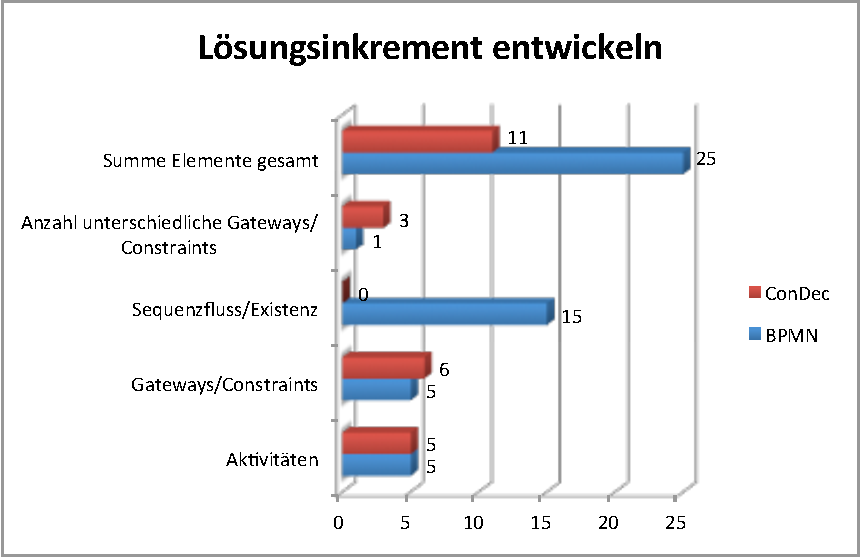
\includegraphics[scale=0.6]{LoesungsinkrementExcel} %pdf, jpg, png...
  \caption{Lösungsinkrement entwickeln}
  \label{fig:LoesungsinkrementExcel}
\end{center}
\end{figure}


Abbildung \ref{fig:OpenUPExcel} kann die Anzahl der Elemente, welche jeweils zur Darstellung des Unterprozesses \grqq Iteration planen und managen\grqq \ notwendig sind, entnommen werden. Sowohl in BPMN, als auch in ConDec werden somit jeweils 11 Aktivitäten benötigt. In BPMN werden keine Gateways und 15 Sequenzflüsse verwendet. In ConDec sind zur korrekten Darstellung 21 Constraints notwendig. Somit werden in BPMN insgesamt 26 Elemente und in ConDec 32 Elemente gebraucht.\newline

\begin{figure}[htp]
\begin{center}
  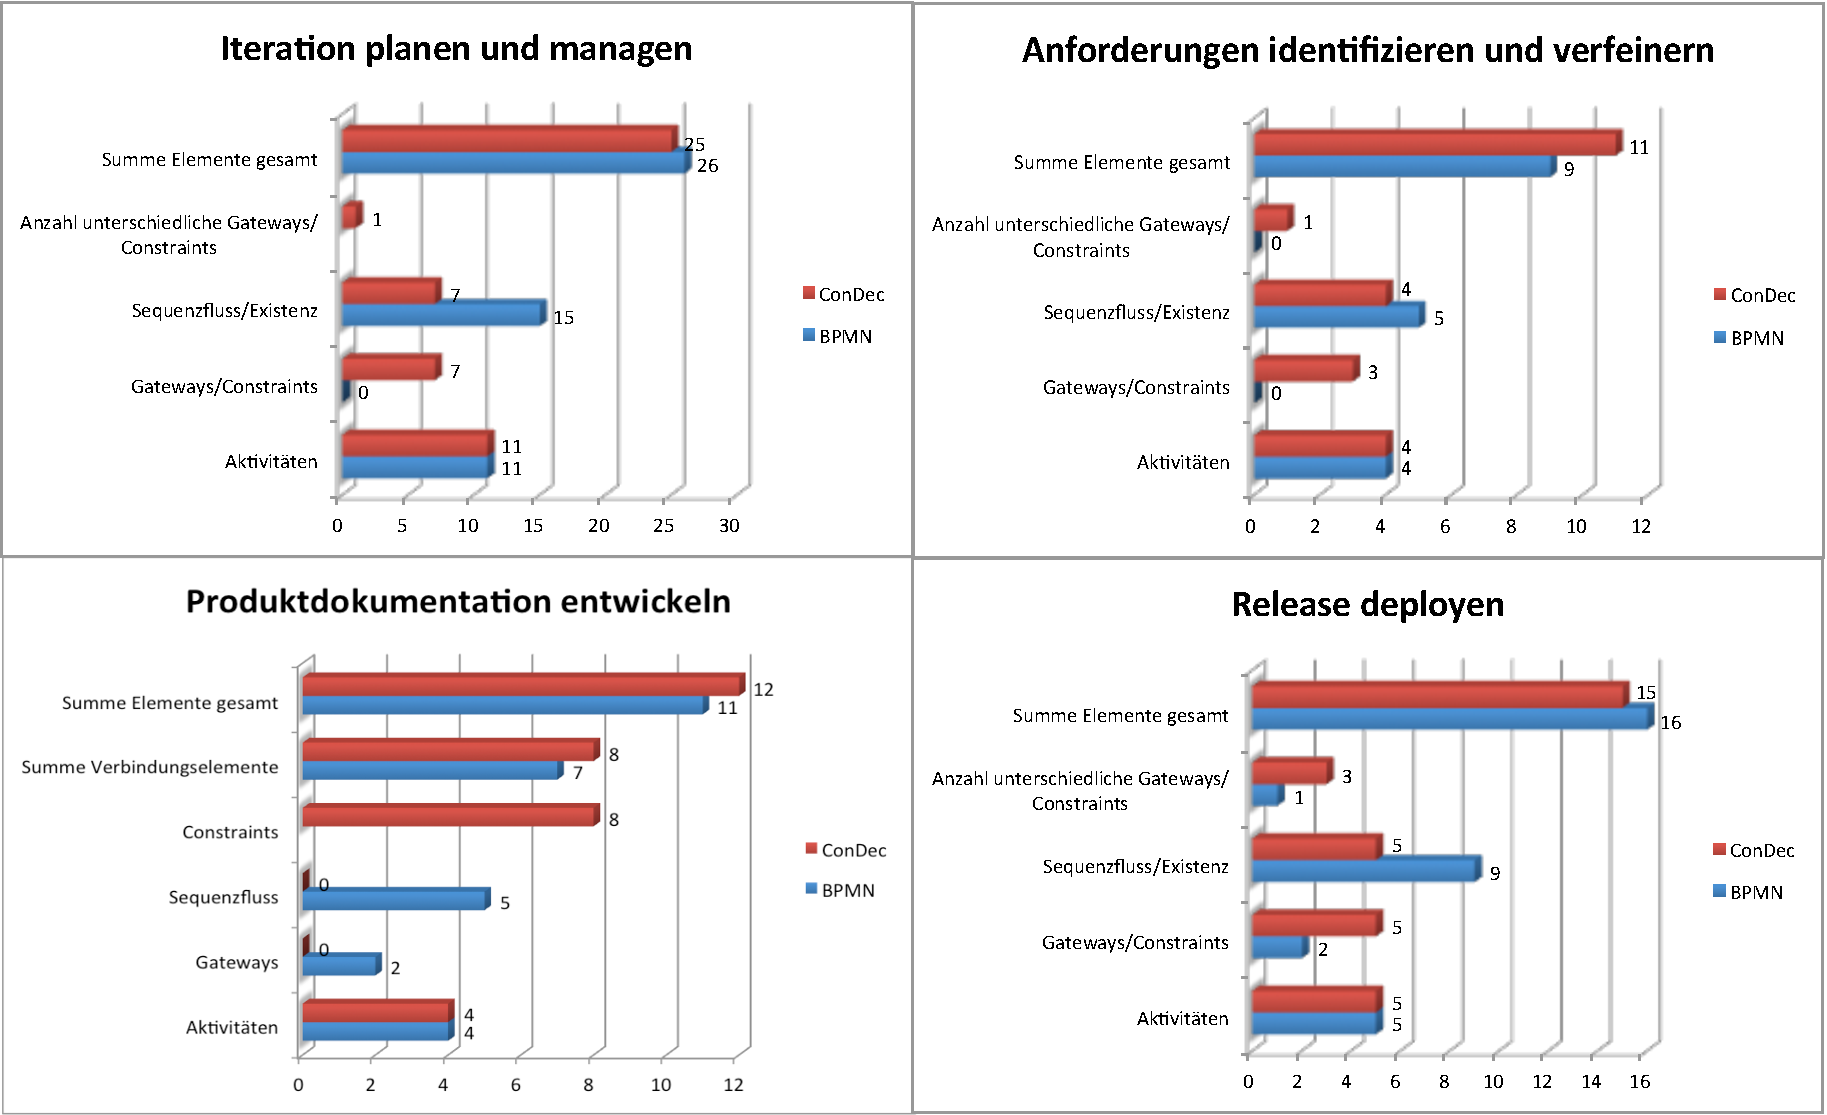
\includegraphics[width=\textwidth]{OpenUPExcel} %pdf, jpg, png...
  \caption{Open UP-Iteration planen}
  \label{fig:OpenUPExcel}
\end{center}
\end{figure}

In Abbildung \ref{fig:OpenUPExcel} sind die Anzahl der Elemente zur Darstellung von \grqq Anforderungen identifizieren und verfeinern\grqq \ abgebildet. Demnach werden sowohl in BPMN, als auch in ConDec jeweils vier Aktivitäten benötigt. Weiterhin sind keine Gateways und 5 Sequenzflusselemente in BPMN zur Darstellung nötig. In ConDec werden drei Constraints verwendet, aber keine unterschiedlichen. Insgesamt werden zur korrekten Abbildung des Metamodells in BPMN neun Elemente und in ConDec 11 Elemente eingesetzt.\newline


Die Anzahl der Elemente zur Darstellung des Prozesses \grqq Produktdokumentation entwickeln\grqq \ kann Abbildung \ref{fig:OpenUPExcel} entnommen werden. Es werden somit jeweils vier Aktivitäten zur Darstellung genutzt. Weiterhin werden in BPMN keine Gateways und sieben Sequenzflusselemente gebraucht. In ConDec sind zur Darstellung sieben Constraints notwendig jedoch keine unterschiedlichen Constraints. Insgesamt werden in BPMN neun Elemente und in ConDec 11 Elemente verwendet.\newline


Wie viele Elemente zur Modellierung des Prozesses \grqq Release deployen\grqq \ benötigt werden, ist in Abbildung \ref{fig:OpenUPExcel} aufgeführt. Jeweils fünf Aktivitäten werden in BPMN und ConDec eingesetzt. In BPMN sind zwei Gateways (keine verschiedenen) und neun Sequenzflusselemente zur Darstellung des Ablaufes notwendig. In ConDec werden hierfür fünf Constraints (drei unterschiedliche)  und fünf Existenz-Constraints benötigt. Somit sind insgesamt 16 Elemente in BPMN und 15 Elemente in ConDec zur Darstellung notwendig. \newline


Der Grundsatz der syntaktischen \textit{Richtigkeit} kann von beiden Prozessmodellierungssprachen eingehalten werden, denn alle imperativen und deklarativen Modelle lassen sich unter Einhaltung der Notationsregeln der jeweiligen Modellierungssprachen erstellen [A 1.1].\newline
Bei dem Grundsatz der semantischen \textit{Richtigkeit} [A 1.2] tritt bei ConDec wiederum das Problem auf, dass Rollen und Artefakte nicht darstellbar sind. Zwar ist dies bei den Phasen des Open UP kein Problem, da hier noch keine Rollen und Artefakte zugeordnet werden, jedoch bei den anderen Prozessen des Open UP (Iteration planen und managen, Anforderungen identifizieren und verfeinern, Produktdokumentation entwickeln und Release deployen). Da hier keine Rollen visualisierbar sind, kann das jeweils im Metamodell enthaltene Verhalten in den ConDec-Modellen nicht vollständig wiedergegeben werden. Hierdurch leidet der Nutzen des Metamodells. \newline
Somit ist BPMN in Bezug auf die \textit{Richtigkeit} die geeignetere Modellierungssprache, da sie beide Anforderungen ([A 1.1] und [A 1.2]) erfüllt und ConDec nur [A 1.1] erfüllt.\newline

Der Grundsatz des \textit{systematischen Aufbaus} [A 2.1] kann wiederum nur von BPMN eingehalten werden, da ConDec keine Möglichkeit bietet, Artefakte im Prozessmodell selbst zu visualisieren.\newline
Auch hier weist BPMN eine bessere Eignung zur Modellierung auf.\newline

Die \textit{Relevanz} [A 3.1] lässt sich nur bei BPMN einhalten, denn es ist wieder bei den in ConDec erstellten Modellen nicht möglich, Rollen und Artefakte zu visualisieren und somit können nicht alle minimal relevanten Informationen im ConDec Modell abgebildet werden..\newline

In Bezug auf die \textit{Klarheit} fällt gerade bei Betrachtung der Modelle der Iterationen \grqq Inception\grqq, \grqq Elaboration\grqq, \grqq Construction\grqq \ und \grqq Transition\grqq \ auf, das bei Modellen, bei denen mehrere Aktivitäten einfach parallel zueinander ablaufen, in BPMN deutlich mehr Sequenzflusselemente zur Darstellung des gleichen Sachverhaltes notwendig sind als Existenz Constraints in ConDec. Zudem werden bei BPMN auch noch jeweils zwei Gateways benötigt. Somit weist BPMN sowohl bei dem einfach gewichteten Punkt Sequenzfluss/Existenz Constraints, als auch bei den doppelt gewichteten Punkten Gateways/Constraints und unterschiedliche Gateways/Constraints eine höhere Anzahl auf als ConDec und bringt somit bei diesen drei Modellen komplexere Modelle hervor [A 4.1]. \newline
Bei der Iteration Transition hingegen weist BPMN nur bei dem einfach gewichteten Punkt Sequenzfluss/Existenz einen höheren Wert auf. Beim doppelt gewichteten Punkt Gateways/Constraints weist das ConDec Modell eine deutlich höhere Anzahl auf. Somit wird hier insgesamt das mit ConDec erstellte Modell leicht komplexer eingestuft als das BPMN-Modell [A 4.1].\newline
Zur Darstellung der  \grqq Phasen des Open UP \grqq \ wird für den Prozess in BPMN beim einfach gewichteten Punkt Sequenzfluss/Existenz eine höhere Anzahl an Sequenzflusselementen benötigt als Existenz Constraints bei ConDec. Ebenso werden bei dem doppelt gewichteten Punkt Gateways/Constraints bei BPMN mehr Elemente verwendet. Beim ebenfalls doppelt gewichteten Punkt unterschiedliche Gateways/Constraints werden bei ConDec mehr Elemente eingesetzt. Somit ist insgesamt das mit BPMN erstellte Modell das leicht komplexere [A 4.1].  \newline
Beim Prozess \grqq Lösungsinkrement entwickeln \grqq \ werden fünf Gateways in BPMN verwendet und bei ConDec werden sechs Constraints benötigt. Bei ConDec werden drei verschiedene Constraints verwendet, bei BPMN jedoch keine verschiedenen Gateways, sondern immer nur das Exklusive Gateway. Somit weist BPMN beim einfach gewichteten Punkt Sequenzfluss/Existenz eine höhere Anzahl auf. Bei den doppelt gewichteten Punkten Gateways/Constraints und unterschiedliche Gateways/Constraints weist ConDec eine höhere Anzahl auf. Dadurch ist in Anbetracht von [A 4.1] das ConDec Modell das komplexere.\newline
Im BPMN Modell ist der Startpunkt durch das Startzeichen gekennzeichnet. Beim ConDec Modell kann kein eindeutiger Start im Modell angegeben werden, da mehrere Aktivitäten als Start infrage kommen [A 4.2]. Dies erhöht die Komplexität des ConDec Modells ebenfalls, da die Aktivitäten, mit welchen gestartet werden kann nicht auf einen Blick erkennbar sind. \newline
Daher kann zusammenfassend gesagt werden, dass die Komplexität des ConDec Modells leicht höher ist, da dies sowohl bei [A 4.1] als auch bei [A 4.2] der Fall ist.\newline
Im Prozess  \grqq Iteration planen und managen\grqq \ gibt es keine Verzweigungen. In ConDec werden sieben Constraints zur Darstellung verwendet. Beim einfach gewichteten Punkt Sequenzfluss/Existenz hat BPMN eine höhere Anzahl. Bei den doppelt gewichteten Punkten Gateways/Constraints und unterschiedliche Gateways/Constraints weist ConDec eine höhere Anzahl auf.\newline
Bei den Prozessen  \grqq Anforderungen identifizieren und verfeinern \grqq \ und  \grqq Produktdokumentation entwickeln \grqq \ weisen die ConDec-Modelle jeweils drei Constraints auf und die BPMN-Modelle keine Gateways. Damit weist BPMN wiederum beim einfach gewichteten Punkt Sequenzfluss/Existenz einen höheren Wert auf und ConDec bei den doppelt gewichteten Punkten Gateways/Constraints und unterschiedliche Gateways/Constraints. Somit ist nach [A 4.1] das BPMN-Modell das weniger komplexe.\newline
Beim Prozess \grqq Release deployen\grqq \ werden in ConDec insgesamt fünf Constraints (drei verschiedene) zur Darstellung des Sachverhaltes benötigt, in BPMN nur zwei Gateways. Somit liegt hier das BPMN-Modell in Bezug auf die Komplexität unter dem ConDec-Modell und ist somit das verständlichere, da es bei den doppelt gewichteten Punkten Gateways/Constraints und unterschiedliche Gateways/Constraints eine geringere Anzahl aufweist [A 4.1].\newline
Somit liegt ConDec bei der Darstellung der Phasen, in denen viele parallele Abläufe dargestellt werden bei der \textit{Klarheit} vorne, während bei den anderen Modellen, bei denen es Schleifen oder Abläufe ohne Verzweigungen zum Darstellen gibt BPMN vorne liegt.\newline

Die \textit{Wirtschaftlichkeit} lässt sich auch beim Open UP bei den Prozessmodellen \grqq Inception\grqq, \grqq Elaboration\grqq, \grqq Construction\grqq \ sowie bei den \grqq Phasen des Open UP\grqq \ mit ConDec besser einhalten, als mit BPMN.  \newline
Bei den anderen Modellen des Open UP jedoch gibt es bei den mit ConDec erstellten Modellen deutlich mehr Constraints und auch unterschiedliche Constraints, als  Gateways bei BPMN. Aus diesem Grund sind hier genau gegensätzlich die ConDec- Modelle komplexer und benötigen somit einen höheren geistigen Aufwand zum Erstellen. \newline
Hierfür gelten die gleichen Argumente wie soeben bei \textit{Klarheit, [A 4.1]} beschrieben [A 5.1]
Somit können hier einerseits mit ConDec bei der Darstellung der \grqq Phasen des Open UP\grqq \ und andererseits bei den anderen Modellen des Open UP die BPMN-Modelle die \textit{Wirtschaftlichkeit} besser erfüllen. Somit kann hier keine der beiden Sprachen als grundsätzlich geeigneter angesehen werden.\newline


Die Abläufe der Diagramme wurden in Signavio und Declare getestet und dadurch ist hier ihre \textit{Vergleichbarkeit} gewährleistet [A 6.1].\newline
Bei der Darstellung der \grqq Phasen des Open UP\grqq \ werden doppelt so viele Elemente in ConDec, wie in BPMN verwendet. Hier ist deshalb die \textit{Vergleichbarkeit} nicht ganz gewährleistet. Bei den anderen Modellen des Open UP unterscheidet sich die Anzahl der Elemente kaum voneinander, wodurch die Vergleichbarkeit hier gewährleistet ist [A 6.2]. \newline
Bei ConDec muss wieder auf die Darstellung von Artefakten und Rollen verzichtet werden, wodurch die \textit{Vergleichbarkeit} der Modelle von ConDec behindert wird. Somit weisen hier beide Prozessmodellierungssprachen Stärken und Schwächen auf [A 6.3].\newline

Eine Zusammenfassung, welche Modellierungssprache bei welchem Grundsatz eher überzeugt hat, kann Abbildung \ref{fig:TabelleOpenUP} entnommen werden. \newline


\begin{figure}[htp]
\begin{center}
  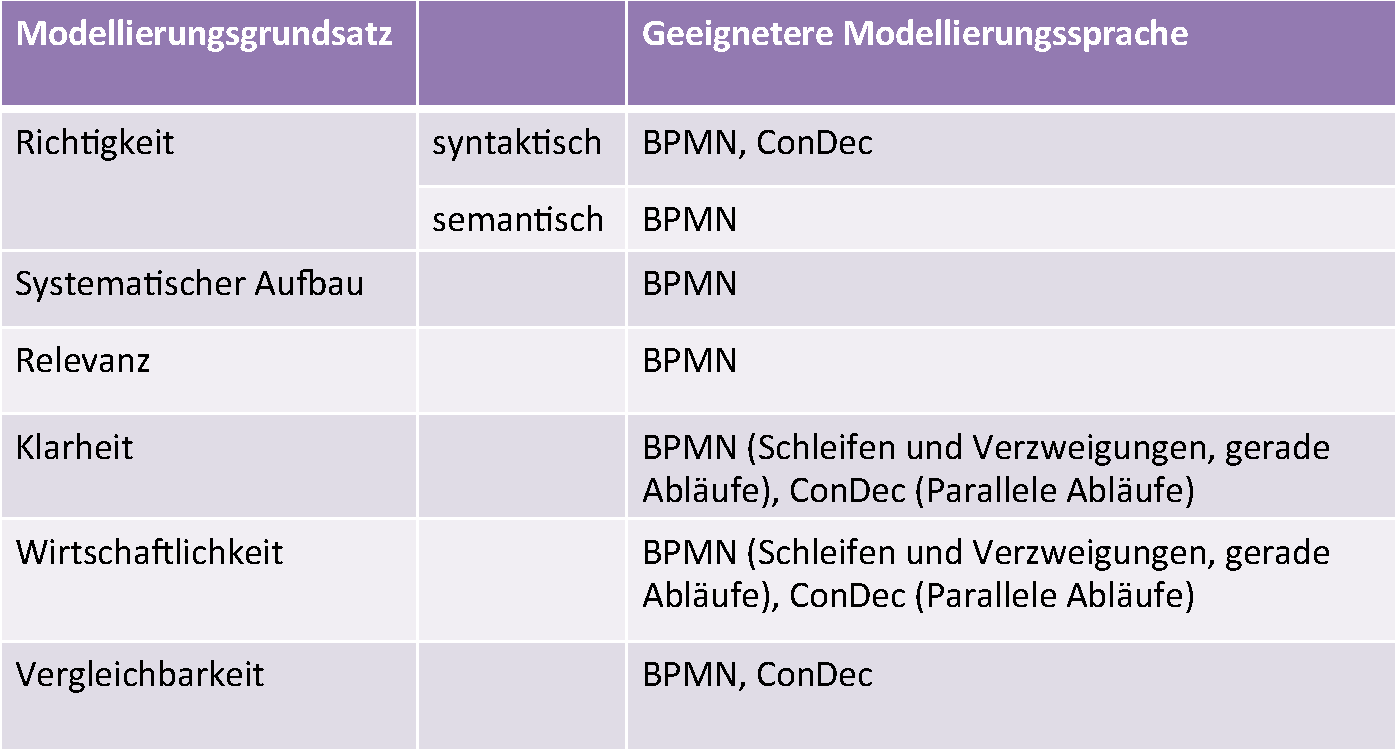
\includegraphics[scale=0.6]{TabelleOpenUP} %pdf, jpg, png...
  \caption{Übersicht Vergleich Open UP}
  \label{fig:TabelleOpenUP}
\end{center}
\end{figure}


\section{V-Modell XT}


Das V-Modell XT zählt zu den schwergewichtigen Prozessmodellen \cite{Hanser2010}. Es wird als Entwicklungsstandard für die Durchführung von IT-Vorhaben in der öffentlichen Verwaltung in Deutschland herangezogen \cite{Kuhrmann2011}. Beschrieben werden im V-Modell XT die Abläufe im Verlauf eines Entwicklungsprojektes über Produkte, Rollen und Aktivitäten \cite{Friedrich2008}. Es wird somit ganz genau geregelt, \textit{Wer}, \textit{Wann}, \textit{Was} in einem Projekt zu tun hat \cite{2004vmodell}. Vorgehensbausteine ermöglichen neben einer Modularisierung der Abläufe auch eine flexible Zusammenstellung, wodurch das V-Modell XT auf die jeweils eigene Situation angepasst werden kann. \cite{Friedrich2008,Zoerner2012}. \newline

\subsection{Analyse V-Modell XT}

Abbildung \ref{fig:grundstruktur} zeigt die Grundstruktur des V-Modell XT. Somit werden beim V-Modell XT verschiedene \textit{Projekttypen} unterschieden, welche wiederum eine passende \textit{Projekttypvariante} haben. das konkrete Vorgehen wird im V-Modell XT durch \textit{Vorgehensbausteine} beschrieben. Welche Vorgehensbausteine in welchem Projekttyp und in welcher Projekttypvariante dann jeweils einzusetzen sind, wird durch den \textit{V-Modell XT Kern und die Vorgehensbausteinlandkarte} festgelegt. Da die Vorgehensbausteine keine Reihenfolge für das Vorgehen angeben, wird dies durch die \textit{Projektdurchführungsstrategie} festgelegt. Zudem werden dort Projektfortschrittsstufen definiert, welche dann bei Erreichen durch \textit{Entscheidungspunkte} markiert werden. Die einzelnen Punkte des V-Modell XT werden nachfolgend detailliert vorgestellt.
\begin{figure}[htp]
\begin{center}
  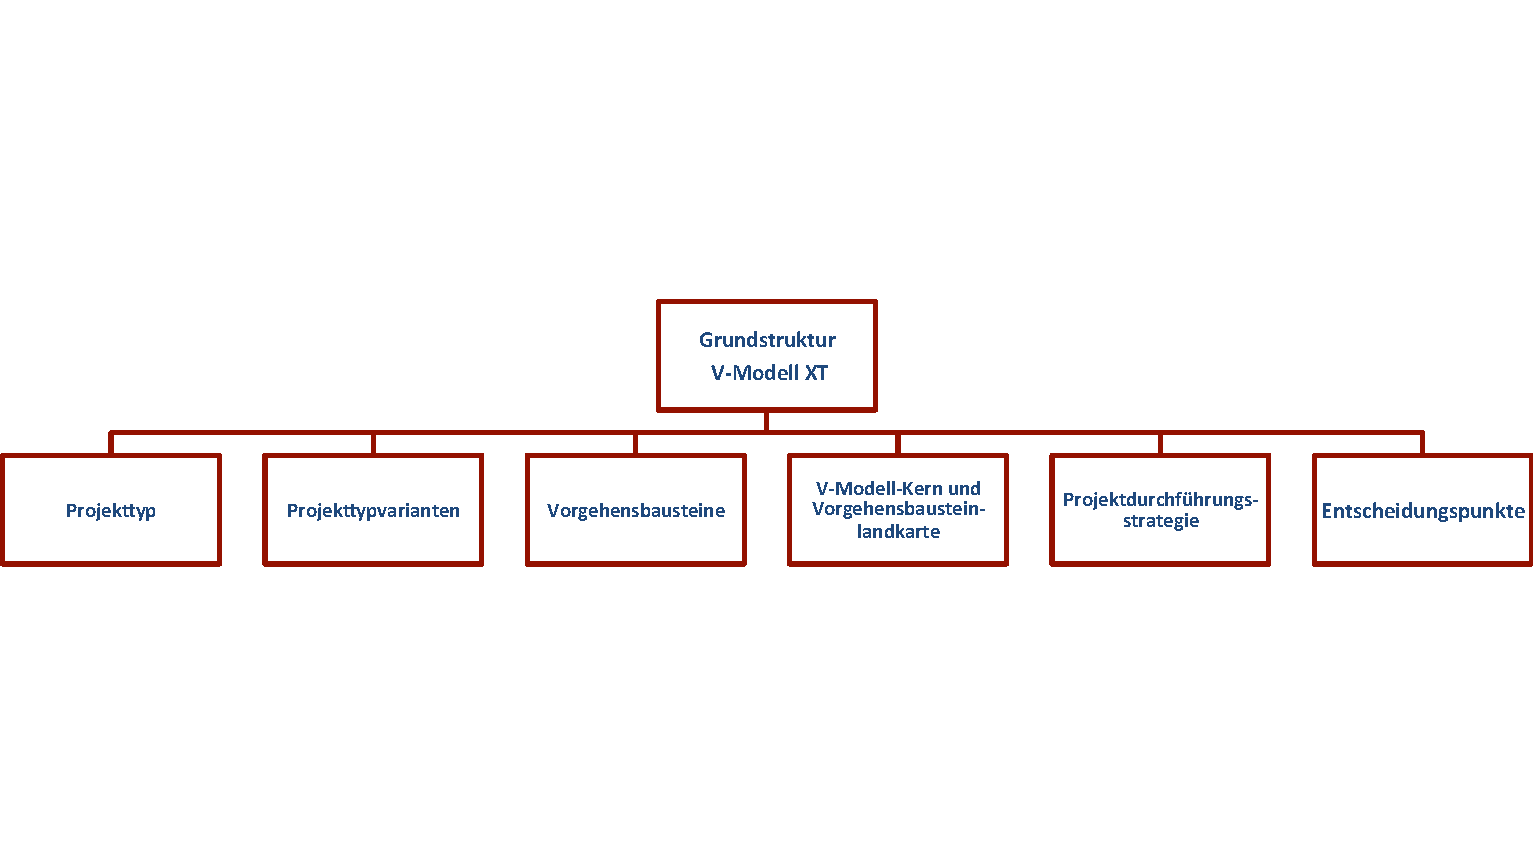
\includegraphics[width=\linewidth]{grundstruktur} %pdf, jpg, png...
  \caption{Grundstruktur V-Modell XT nach \cite{2004vmodell}}
  \label{fig:grundstruktur}
\end{center}
\end{figure}

\subsubsection{Projekttypen}
Nicht alle V-Modell-Projekttypen laufen nach exakt demselben Schema ab. Auf Grund ihrer charakteristischen Eigenschaften lassen sie sich demnach in unterschiedliche Projekttypen einteilen. Abbildung \ref{fig:Projekttypen} gibt einen ersten Überblick über die verschiedenen Projekttypen im V-Modell XT \cite{2004vmodell}.

\begin{figure}[htp]
\begin{center}
  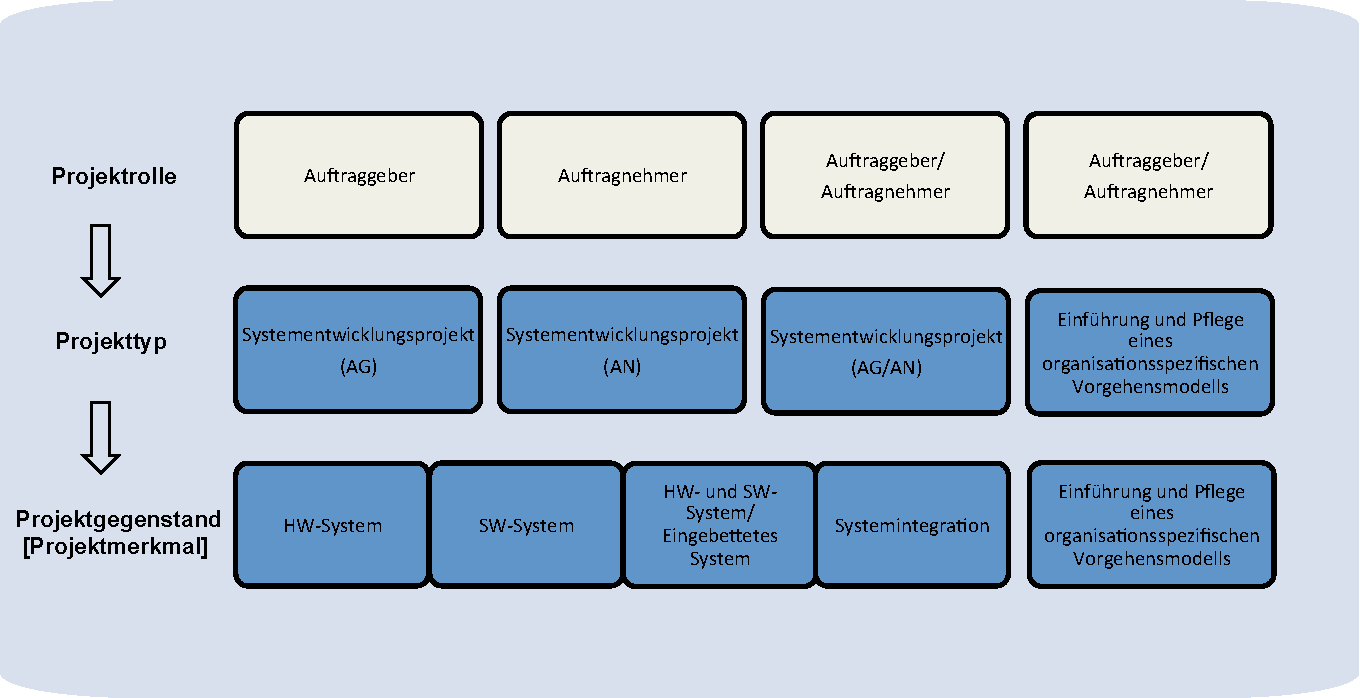
\includegraphics[width=\linewidth]{v-modell-rollen} %pdf, jpg, png...
  \caption{Projekttypen V-Modell XT nach \cite{2004vmodell}}
  \label{fig:Projekttypen}
\end{center}
\end{figure}

Es existieren somit vier verschiedene Projekttypen: \grqq Systementwicklungsprojekt eines Auftraggebers\grqq, \grqq Systementwicklungsprojekt eines Auftragnehmers\grqq, \grqq Systementwicklungsprojekt eines Auftraggebers/Auftragnehmers\grqq \ und \grqq Einführung und Pflege eines organisationsspezifischen Vorgehensmodells\grqq \ \cite{reinhard2008}. \newline

Es werden drei verschiedene Projektrollen unterschieden, welche dem jeweiligen Projekttyp entsprechen: In der Rolle \textit{Auftragnehmer} wird ein vom \textit{Auftraggeber} spezifiziertes System entwickelt. Die Systementwicklung wird an einen oder mehrere \textit{Arbeitnehmer} weiter gegeben, wenn man sich in der Rolle \textit{Arbeitgeber} befindet. Das System  wird selbst entwickelt in der Rolle \grqq Auftraggeber/Auftragnehmer\grqq \ \cite{brack2010,2004vmodell}.\newline


Beim \grqq Systementwicklungsprojekt eines Auftraggebers\grqq \ wird die Entwicklung des Projektgegenstandes im Projektverlauf  ausgeschrieben und der Auftragnehmer trifft eine Auswahl anhand der eingehenden Angebote. Der Auftragnehmer, welcher für die Entwicklung des Projektgegenstandes ausgewählt wurde, entwickelt den Projektgegenstand, welcher dann vom Auftragnehmer abgenommen wird \cite{reinhard2008,2004vmodell}.\newline
Umgekehrt wird beim \grqq Systementwicklungsprojekt eines Auftragnehmers\grqq \ im Laufe des Projektes ein Angebot erstellt und bei Auswahl durch den Auftraggeber ein Projektgegenstand entwickelt, welcher abschließend an den Auftraggeber ausgeliefert und von diesem abgenommen wird \cite{reinhard2008,2004vmodell}.\newline
Bei \grqq Einführung und Pflege eines organisationsspezifischen Vorgehensmodells\grqq \ geht es um Projekte, welche Prozessmodelle z.B. das V-Modell einführen und verbessern wollen. Für diesen Zweck ist eine Analyse des vorherigen Prozessmodelles notwendig und etwaige Verbesserungsmöglichkeiten sind zu erfassen und durchzuführen \cite{reinhard2008,2004vmodell}.\newline
Wie aus Abbildung \ref{fig:Projekttypen} ersichtlich ist, kann es sich im V-Modell XT beim Projektgegenstand um ein Hardware (HW)-System, ein Software (SW)-System, ein eingebettetes System oder eine Systemintegration handeln \cite{brack2010,2004vmodell}. \newline

\subsubsection{Projekttypvarianten}
Für jeden der Projekttypen, gibt es im V-Modell XT mindestens eine passende Projekttypvariante. Diese bestimmt die Rahmenbedingungen für mögliche Abläufe eines Projektes. In Abbildung \ref{fig:Projekttypvarianten} sind die verschiedenen Projekttypvarianten des V-Modell XT aufgelistet und es wird gezeigt, mit welchen Merkmalen die zugehörigen Projekttypvarianten ausgewählt werden können \cite{2004vmodell}.   
\begin{figure}[htp]
\begin{center}
  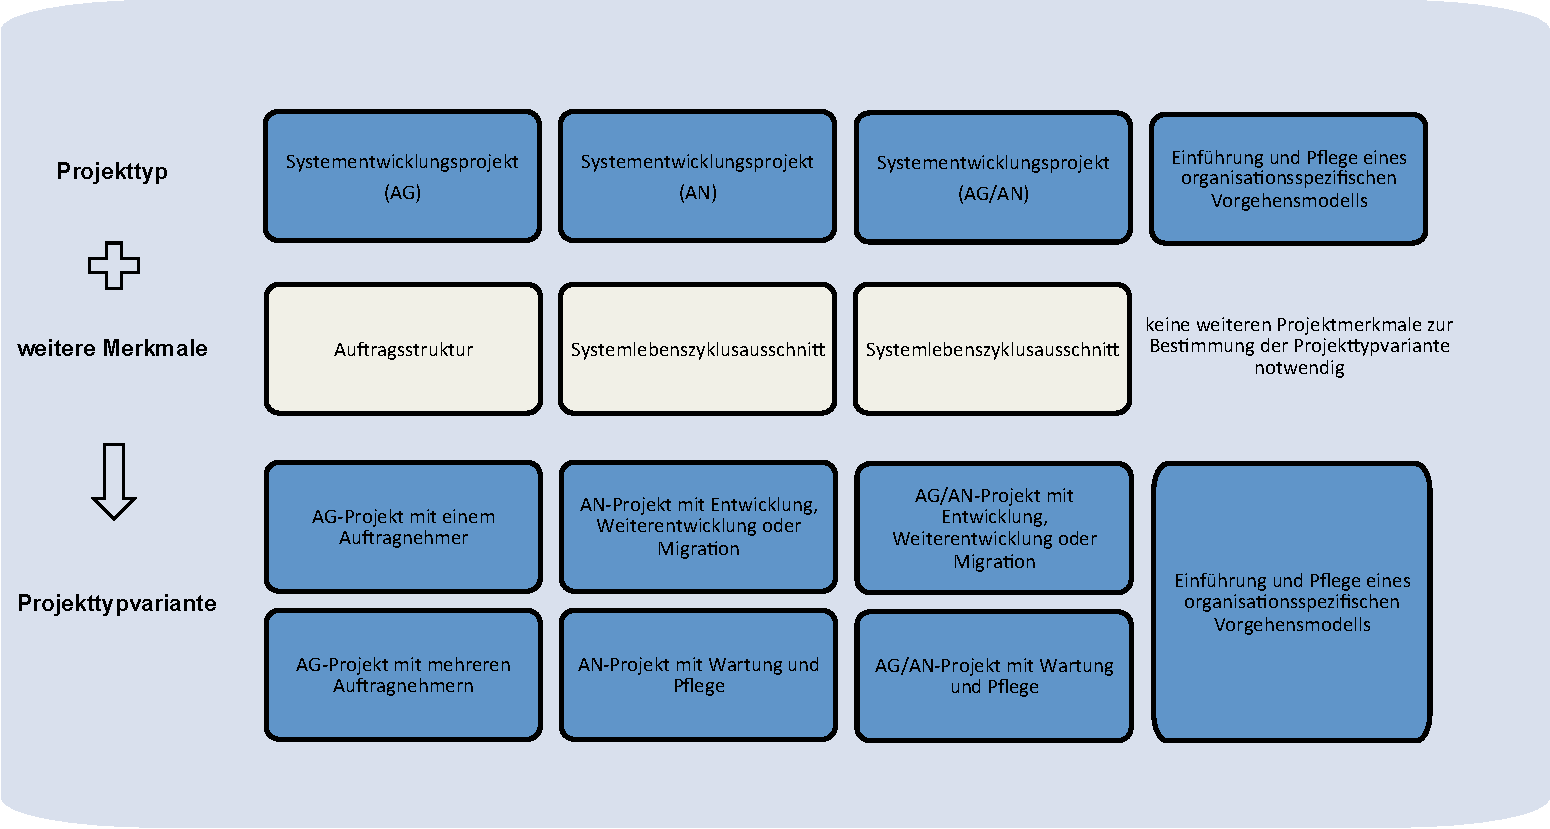
\includegraphics[width=\linewidth]{Projekttypvarianten-v-modell} %pdf, jpg, png...
  \caption{Zuordnung der Projekttypvarianten zu den Projekttypen des V-Modell XT \cite{2004vmodell}}
  \label{fig:Projekttypvarianten}
\end{center}
\end{figure}

Für den Projekttyp \grqq Systementwicklungsprojekt (AG)\grqq \ existieren zwei verschiedene Projekttypvarianten, welche je nach \grqq Auftragsstruktur\grqq \ ausgewählt werden. Falls der Auftraggeber mit nur einem Auftragnehmer zusammen arbeitet, ergibt sich die Projekttypvariante \grqq Systementwicklungsprojekt (AG)- Projekt mit einem Auftragnehmer\grqq. Arbeitet der Auftraggeber mit mehreren Auftragnehmern zusammen, ergibt sich die Projekttypvariante \grqq Systementwicklungsprojekt (AG)- Projekt mit mehreren Auftragnehmern\grqq \ \cite{2004vmodell}.\newline
Bei den Projekttypen \grqq Systementwicklungsprojekt (AN)\grqq \ und \grqq Systementwicklungsprojekt (AG/AN)\grqq \ wird die Unterscheidung anhand des Systemlebenszyklusausschnitt des Projektes durchgeführt. Somit wird in den Systemlebenszyklusausschnitten Entwicklung, Weiterentwicklung und Migration eine andere Projekttypvariante gewählt als in Wartung und Pflege \cite{2004vmodell}.\newline 
Für den Projekttyp \grqq Einführung und Pflege eines organisationsspezifischen Vorgehensmodells\grqq \ existiert nur eine einzige Projekttypvariante, weshalb hier keine weiteren Merkmale zur Bestimmung der Projekttypvariante notwendig sind \cite{2004vmodell}.\newline

  
 \subsubsection{Vorgehensbausteine}
Modulare, aufeinander aufbauende Vorgehensbausteine, bilden den Kern des V-Modell XT. Vorgehensbausteine sind selbständig entwickelbare und änderbare Einheiten und bestehen aus Aktivitäten, Produkten und Rollen. Sie geben einerseits vor, \grqq Was\grqq{}  in einem Projekt zu tun ist, also welche Produkte zu erstellen sind und andererseits \grqq Wer\grqq, also welche konkrete Rolle für das jeweilige Produkt verantwortlich ist. Abbildung \ref{fig:vorgehensbausteine} gibt einen Überblick über diese \cite{ruf2008, 2004vmodell}.\newline

\begin{figure}[htp]
\begin{center}
  \includegraphics[width=\linewidth]{vorgehensbaustein} %pdf, jpg, png...
  \caption{Vorgehensbausteine V-Modell XT nach \cite{2004vmodell}}
  \label{fig:vorgehensbausteine}
\end{center}
\end{figure}

Ergebnisse und Zwischenergebnisse werden Produkte genannt. Komplexe Produkte können in ein oder mehrere Themen gegliedert werden und inhaltlich zusammengehörende Produkte können zu einer Disziplin zusammengefasst werden. Produkte können hierbei auch voneinander abhängig sein, sowohl innerhalb eines Vorgehensbausteins, als auch zwischen verschiedenen Vorgehensbausteinen \cite{2004vmodell}.\newline
Jedes Produkt wird von genau einer Aktivität fertig gestellt. Aktivitäten legen auch fest, wie die einzelnen Produkte zu bearbeiten sind. Sie bestehen aus einer oder mehreren Teilaktivitäten, sogenannten Arbeitsschritten. Diese stellen eine Art Arbeitsanleitung dar und bearbeiten eine oder mehrere Themen \cite{2004vmodell}.\newline
Durch Rollen werden eine Menge von Aufgaben und Verantwortlichkeiten gekapselt, wodurch das V-Modell XT unabhängig von organisatorischen Rahmenbedingungen bleibt. Eine Zuordnung von Personen bzw. Organisationseinheiten zu einer Rolle erfolgt erst zu Beginn eines Projektes. Es wird jedem Produkt genau eine Rolle als Verantwortlicher zugewiesen. Weitere Rollen können am Produkt als Mitwirkende mitarbeiten \cite{2004vmodell}. \newline



\subsubsection{V-Modell XT-Kern und Vorgehensbausteinlandkarte}

Um ein spezifisches Projekt an ein V-Modell XT-Projekt anzupassen, ist für jeden Projekttyp und jede Projekttypvariante genau vorgegeben, welche Vorgehensbausteine jeweils anzuwenden sind \cite{2004vmodell}. Hierdurch kann also ein individuelles V-Modell XT für ein Projekt erstellt werden \cite{heinrich2007}. Hierfür ist es notwendig, die Vorgehensbausteine für ein V-Modell XT-Projekt nach den Vorgaben des Projekttyps auszuwählen und festzulegen \cite{2004vmodell}. \newline

\begin{figure}[htp]
\begin{center}
  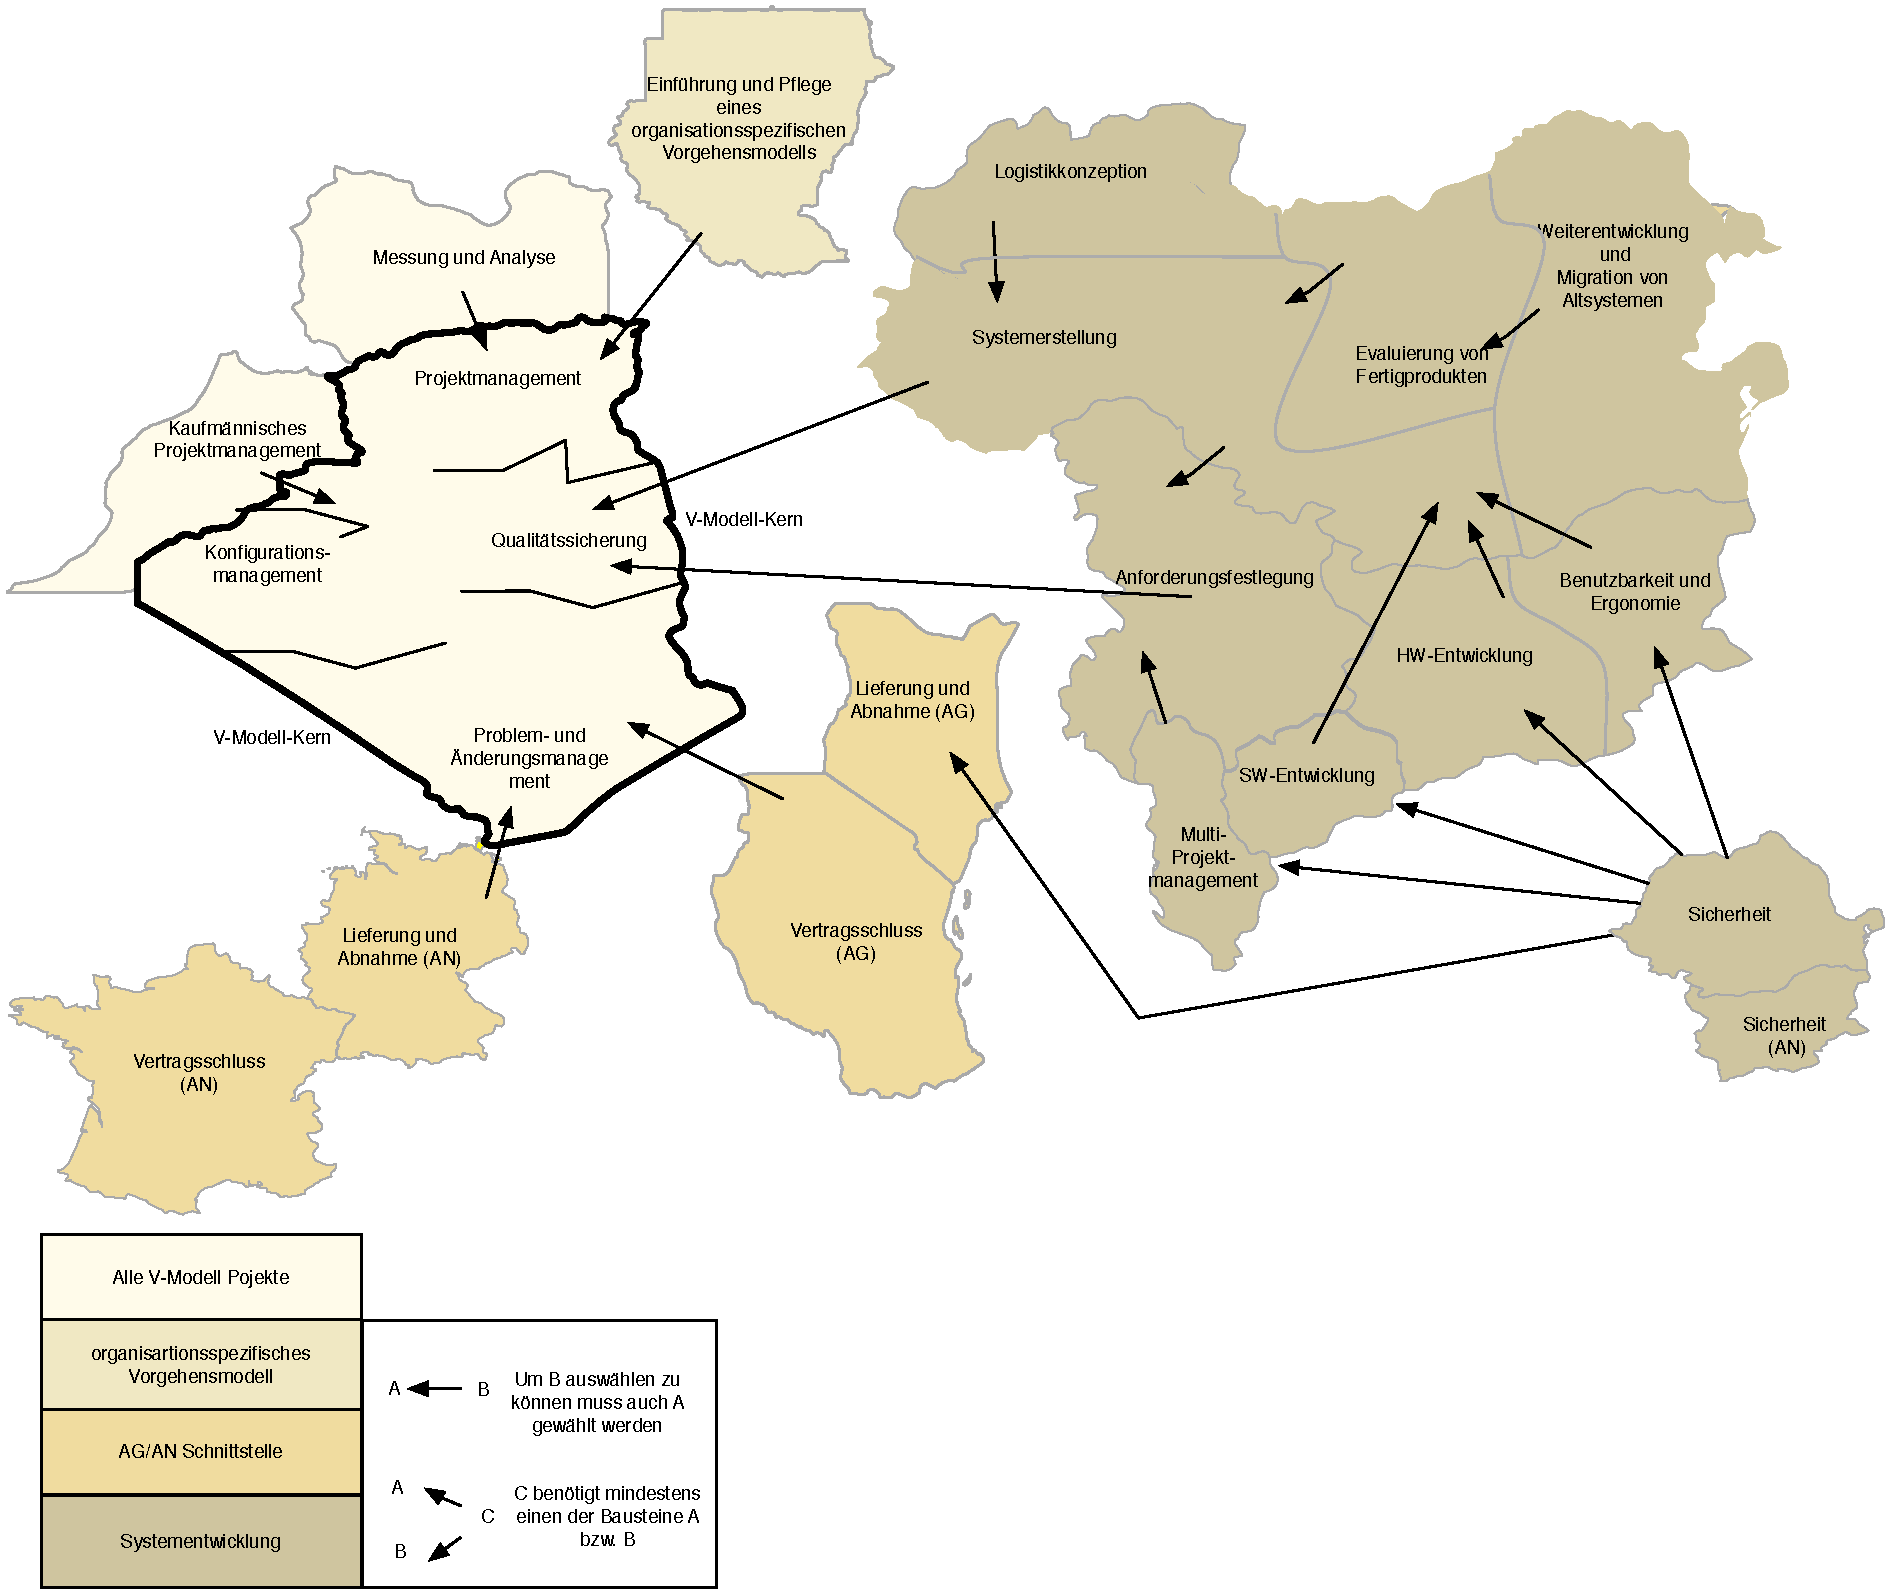
\includegraphics[width=\linewidth]{landkarte} %pdf, jpg, png...
  \caption{V-Modell XT-Kern und Vorgehensbausteinlandkarte nach \cite{2004vmodell}}
  \label{fig:landkarte}
\end{center}
\end{figure}

 Wie Abbildung \ref{fig:landkarte} zeigt, können die Vorgehensbausteine in die vier Bereiche \grqq Alle V-Modell XT-Projekte\grqq, \grqq Organisationsspezifisches Vorgehensmodell, \grqq AG/AN-Schnittstelle und \grqq Systementwicklung\grqq \  eingeteilt werden \cite{2004vmodell}.\newline
 Im Bereich \grqq Alle V-Modell XT-Projekte\grqq \ finden sich diejenigen Vorgehensbausteine, welche in jedem V-Modell XT-Projekt herangezogen werden können. Zudem gibt es den V-Modell XT-Kern, in welchem sich die Vorgehensmodelle finden, die in jedem V-Modell XT-Projekt unerlässlich sind: \grqq Projektmanagement\grqq, \grqq Konfigurationsmanagement\grqq, \grqq Problem- und Änderungsmanagement\grqq \ und \grqq Qualitätssicherung\grqq. Zusätzlich zu diesen verpflichtenden Vorgehensbausteinen können in jedem Projekt noch \grqq Kaufmännisches Projektmanagement\grqq, welches bei der Integration des Projektmanagements in das kaufmännische Management hilft und \grqq Messung und Analyse\grqq, welches Verfahren für die organisationsweite und projektübergreifende Erfassung und Auswertung von Kennzahlen bereitstellt, verwendet werden \cite{2004vmodell}.\newline
 Ist der Zweck eines Projektes die Entwicklung eines \grqq Organisationsspezifischen Vorgehensmodells\grqq, so muss der Vorgehensbaustein \grqq Einführung und Pflege eines organisationsspezifischen Vorgehensmodells\grqq \ hinzugenommen werden. In diesem finden sich Verfahren und Richtlinien für die Einführung eines Vorgehensmodells innerhalb einer Organisation sowie die damit einhergehende Etablierung eines stetigen Verbesserungsprozesses \cite{2004vmodell}.\newline
 Wenn ein Projekt die Entwicklung eines Systems zum Ziel hat, so wird der Bereich \textit{Systementwicklung} herangezogen. In diesem befinden sich die Vorgehensbausteine \grqq Anforderungsfestlegung\grqq, \grqq Systemerstellung\grqq, \grqq HW-Entwicklung\grqq, \grqq SW-Entwicklung\grqq, \grqq Logistikkonzeption\grqq, \grqq Weiterentwicklung und Migration von Altsystemen\grqq, \grqq Evaluierung von Fertigprodukten\grqq, \grqq Benutzbarkeit und Ergonomie\grqq, \grqq Sicherheit\grqq \ sowie \grqq Sicherheit (AN)\grqq \ und \grqq Multi-Projektmanagement\grqq \ \cite{2004vmodell}. \newline
 Im Bereich \grqq AG/AN-Schnittstelle\grqq \ befinden sich die Vorgehensbausteine für die Kommunikation zwischen Arbeitgeber und Arbeitnehmer: \grqq Lieferung und Abnahme (AG)\grqq, \grqq Lieferung und Abnahme (AN)\grqq, \grqq Vertragsschluss (AG)\grqq \ und \grqq Vertragsschluss (AN)\grqq. Hier finden sich Regelungen über den Vertrag zwischen Arbeitgeber und Arbeitnehmer sowie über Lieferung und Abnahme des Entwicklungsgegenstandes \cite{2004vmodell}. \newline
 
 \subsubsection{Projektdurchführungsstrategie}
 Die Vorgehensbausteine im V-Modell XT geben zwar an, welche Produkte jeweils zu erstellen und welche Aktivitäten durchzuführen sind, sie geben jedoch hierbei nicht vor, in welcher Reihenfolge dies geschehen soll. Damit das Projekt trotzdem geplant und gesteuert werden kann, gibt es im V-Modell XT eine Projektdurchführungsstrategie welche auf den jeweiligen Projekttyp und die Projekttypvariante abgestimmt ist. Hier wird somit die Reihenfolge der Produkte und Aktivitäten festgelegt, also das  \grqq Wann\grqq {} festgelegt. Außerdem werden hier zu erreichende Projektfortschrittsstufen vorgegeben \cite{2004vmodell}. \newline
 
 \subsubsection{Entscheidungspunkte}
Abbildung \ref{fig:entscheidungspunkte} zeigt, dass die in der Projektdurchführungsstrategie vorgegebenen Projektfortschrittsstufen bei Erreichen durch Entscheidungspunkte markiert werden. Diese stellen einen Meilenstein im Projektablauf dar. Um den Entscheidungspunkt zu erreichen, muss eine vorgegebene Menge an Produkten fertig gestellt werden. Hier entscheidet das Projektmanagement über das Erreichen der Projektfortschrittsstufe und das Freigeben des nächsten Projektabschnitts. Die Entscheidungspunkte, welche im V-Modell XT erreicht werden müssen können Abbildung \ref{fig:v-modell} entnommen werden. Diese werden wie im V-Modell XT-Kern in die vier Bereiche \grqq Alle V-Modell XT-Projekte\grqq, \grqq Organisationsspezifisches Vorgehensmodell\grqq, \grqq AG/AN-Schnittstelle\grqq \ und \grqq Systementwicklung\grqq \ unterschieden \cite{2004vmodell}. \newline
Demnach gelten die Entscheidungspunkte \grqq Projekt genehmigt\grqq, \grqq Projekt definiert, \grqq Iteration geplant\grqq \ und \grqq Projekt abgeschlossen\grqq \ für alle Projekttypen und Projektdurchführungsstrategien \cite{2004vmodell}. \newline
Bei der Systementwicklung werden die Entscheidungspunkte \grqq Anforderungen festgelegt\grqq, \grqq System spezifiziert\grqq, \grqq System entworfen\grqq, \grqq Feinentwurf abgeschlossen\grqq, \grqq Systemelemente realisiert\grqq \ und \grqq System integriert\grqq \ verwendet. Falls das Projekt vor der Anforderungserhebung in mehrere Teilmodelle aufgeteilt werden soll, werden zusätzlich die Entscheidungspunkte \grqq Gesamtprojekt aufgeteilt\grqq \ und \grqq Gesamtprojektfortschritt überprüft\grqq \ hinzugenommen \cite{2004vmodell}. \newline
Die Entscheidungspunkte für die Arbeitgeber/Arbeitnehmer Schnittstelle setzen sich aus \grqq Projekt ausgeschrieben\grqq, \grqq Angebot abgegeben\grqq, \grqq Projekt beauftragt\grqq, \grqq Lieferung durchgeführt\grqq, \grqq Abnahme erfolgt\grqq \ und \grqq Projektfortschritt überprüft\grqq \ zusammen \cite{2004vmodell}. \newline
 Bei der Entwicklung eines organisationsspezifischen Vorgehensmodells kommen die Entscheidungspunkte \grqq Vorgehensmodell analysiert\grqq, \grqq Verbesserung Vorgehensmodell konzipiert\grqq \ und \grqq Verbesserung Vorgehensmodell realisiert\grqq \ zum Einsatz \cite{2004vmodell}. \newline
 Die Entscheidungspunkte legen das \grqq Wann\grqq {} und \grqq Was\grqq {} fest, d.h. wann welche Produkte fertig gestellt sein müssen.

 
 
 \begin{figure}[!htbp]
\begin{center}
  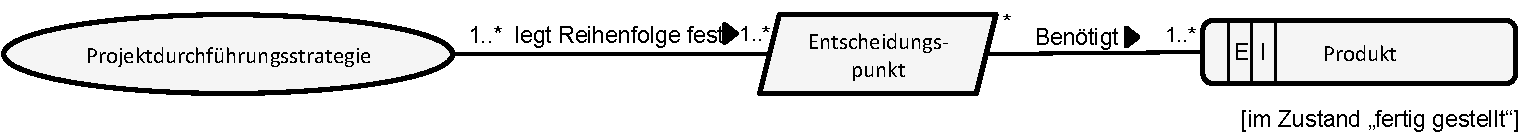
\includegraphics[width=\linewidth]{Entscheidungspunkte} %pdf, jpg, png...
  \caption{Entscheidungspunkte V-Modell XT nach \cite{2004vmodell}}
  \label{fig:entscheidungspunkte}
\end{center}
\end{figure}
 
\begin{sidewaysfigure}[!htbp]
\begin{center}
  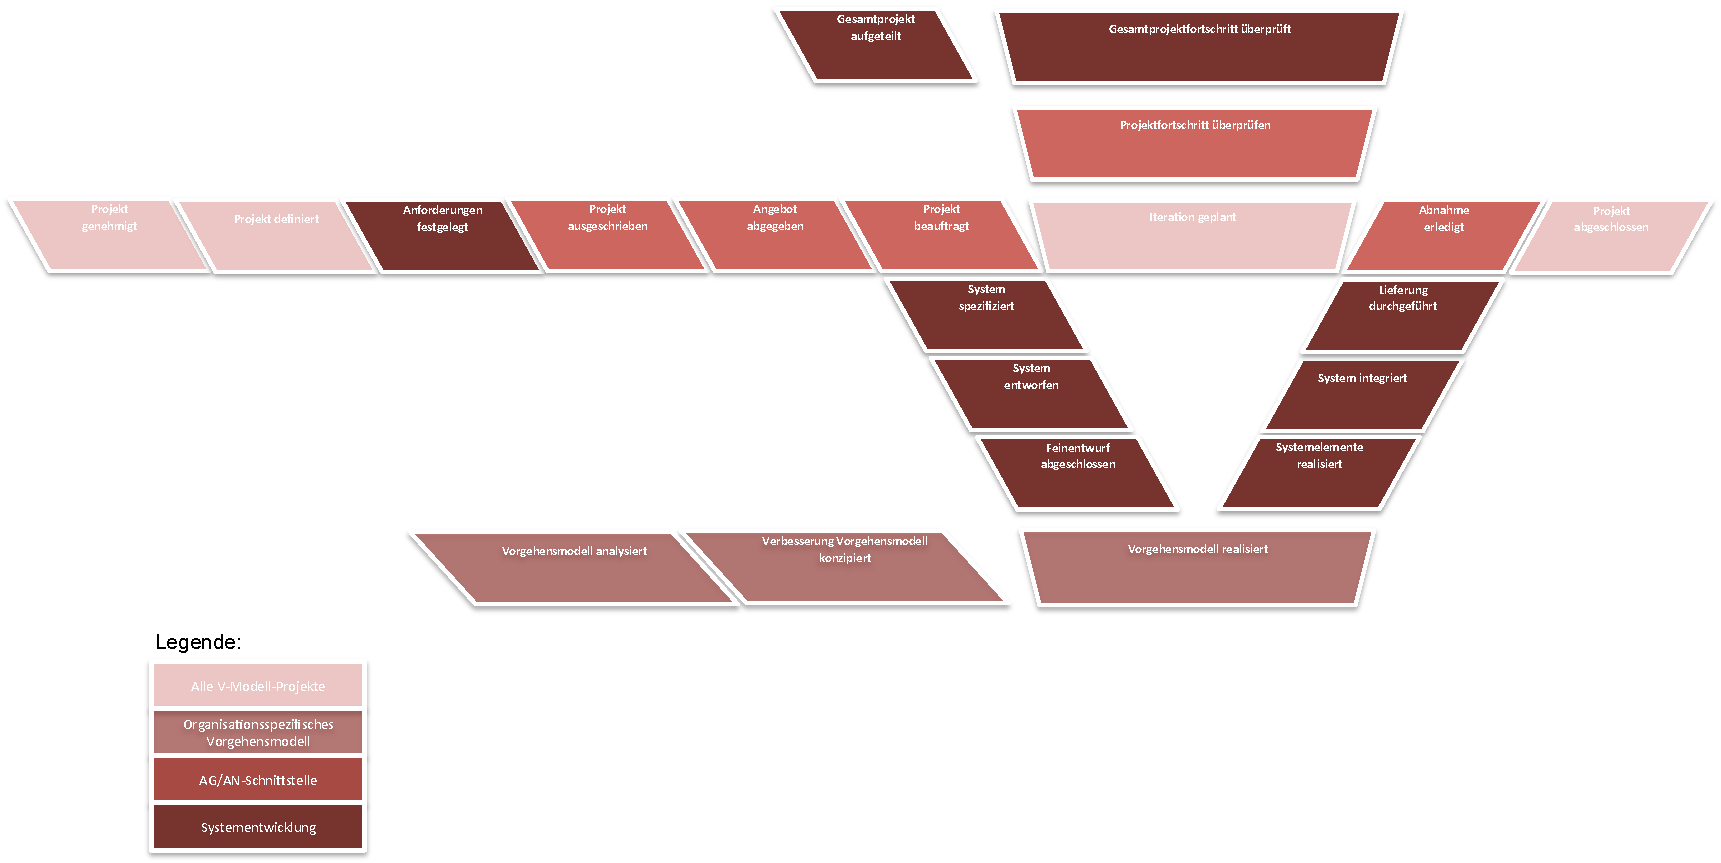
\includegraphics[width=\linewidth]{v-modell} %pdf, jpg, png...
  \caption{Entscheidungspunkte für die Projektdurchführungsstrategie nach \cite{2004vmodell}}
  \label{fig:v-modell}
\end{center}
\end{sidewaysfigure}


\clearpage

\subsection{Imperative Modellierung V-Modell XT}

Im Folgenden werden Teile des V-Modells XT modelliert da das ganze V-Modell XT den Rahmen dieser Arbeit sprengen würde. Aus diesem Grund wird zum Einen das \grqq Systementwicklungsprojekt AG/AN\grqq \ ausgewählt. Weiterhin wird ein hierzu gehöriger Unterprozess \grqq Inkrementelle Entwicklung\grqq \ und die hierzu gehörenden Unterprozesse \grqq System entwerfen\grqq \ und \grqq System spezifizieren\grqq \ modelliert.

\subsubsection{Systementwicklungsprojekt AG/AN}


Die imperative Modellierung des Prozesses \grqq Systementwicklungsprojekt AG/AN\grqq \ zeigt Abbildung \ref{fig:Systementwicklungimp}. \newline
Zunächst muss ein Projekt genehmigt und definiert werden. Dies ist durch die einander folgenden Aktivitäten \grqq Projekt genehmigen\grqq \ und \textit{Projekt definieren} dargestellt.\newline
In der nachfolgenden Aktivität müssen sodann die \grqq Anforderungen festgelegt werden\grqq, bevor die \grqq Iteration geplant\grqq \ werden kann. \newline
Hiernach muss entschieden werden, ob eine \grqq Prototypische Entwicklung durchgeführt\grqq, eine \grqq Komponentenbasierte Entwicklung durchgeführt\grqq \ oder eine \grqq Inkrementelle Entwicklung durchgeführt\grqq \ werden soll. Dies wird durch das Exklusive Gateway beschrieben, welches nur eine Alternative zulässt.\newline
Anschließend wird das \grqq System abgenommen\grqq. An dieser Stelle wird entschieden, ob erneut zu \grqq Anforderungen festlegen\grqq \ zurückgekehrt wird und der Prozess ab dieser Aktivität erneut startet oder ob zu \grqq Projekt ausschreiben\grqq \ zurückgekehrt wird und der Prozess ab hier erneut startet. Ansonsten endet der Prozess mit der Aktivität \grqq Projekt abschließen\grqq.

\begin{figure}[!htbp]
\begin{center}
  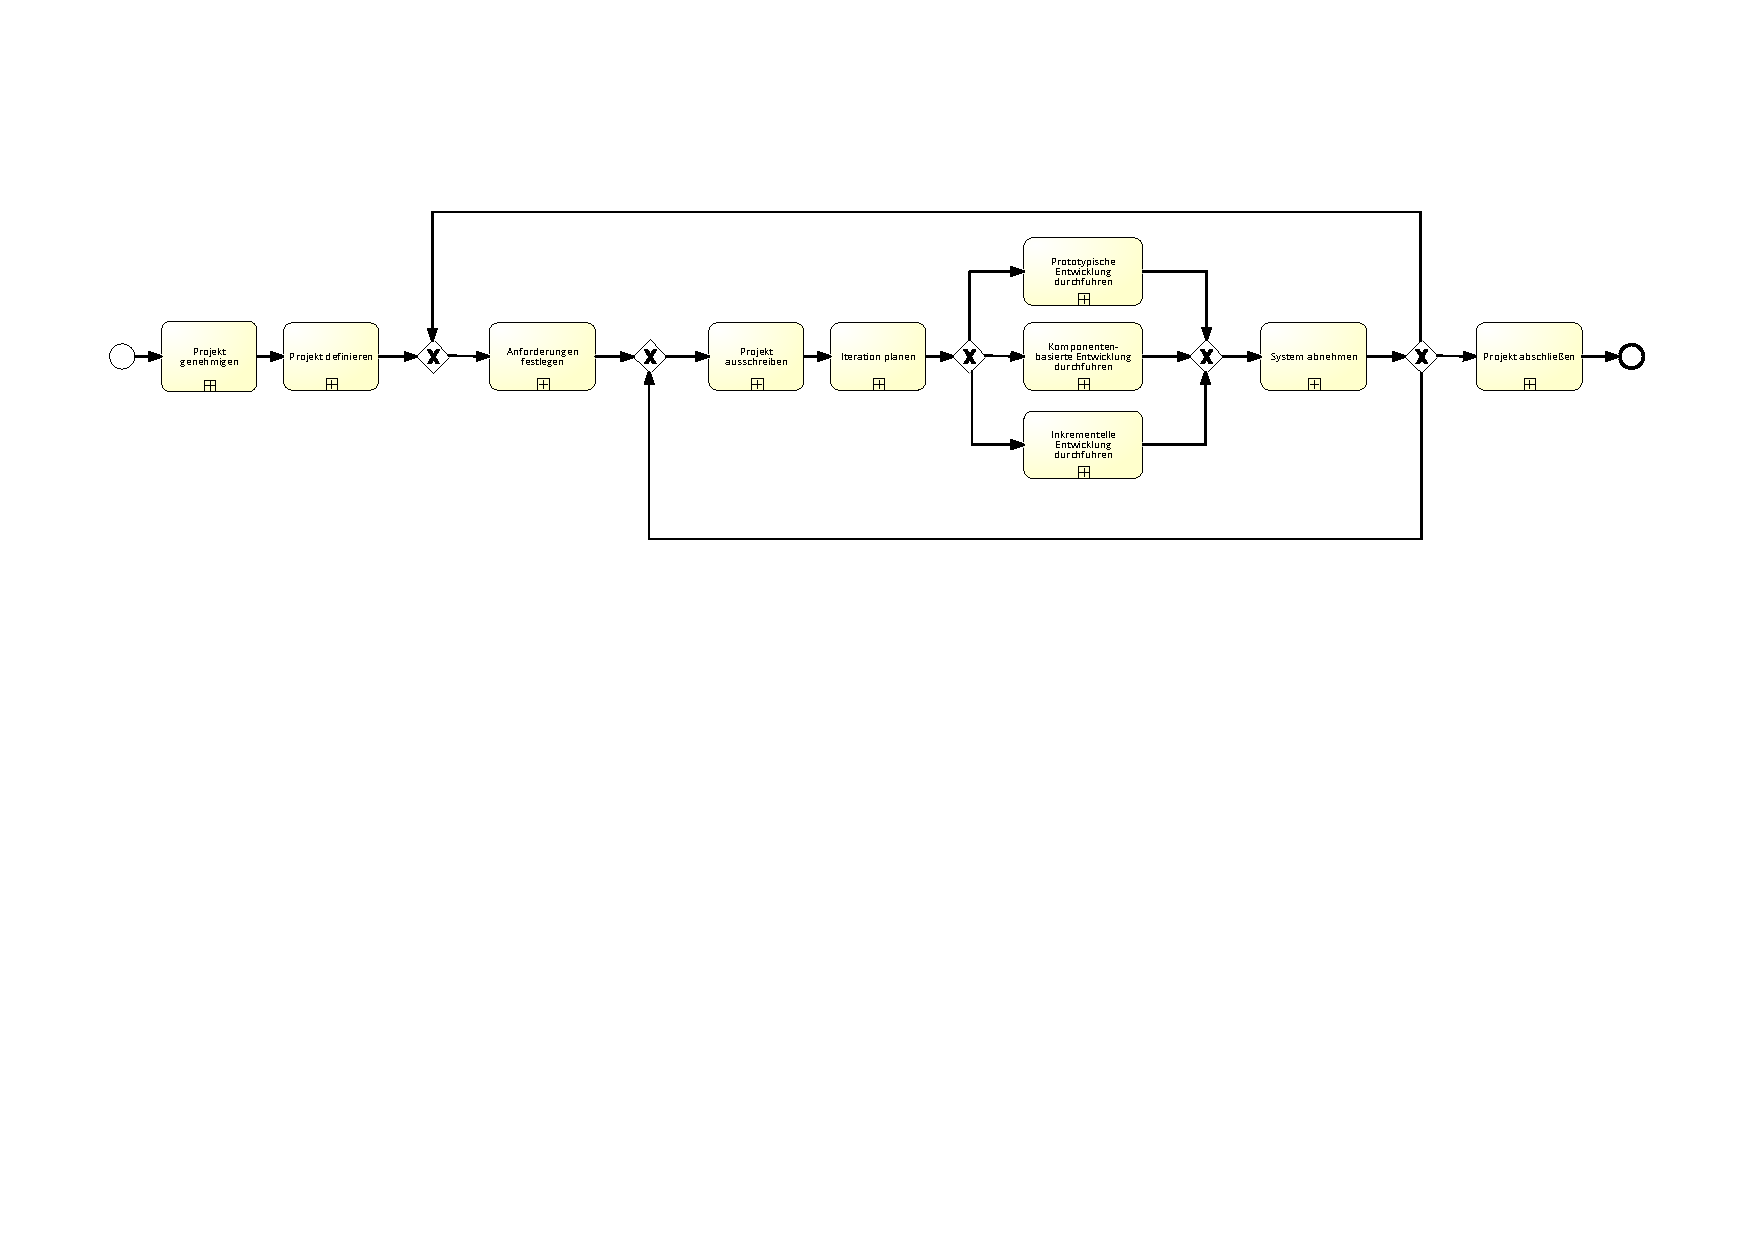
\includegraphics[width=\linewidth]{Systementwicklungimp} %pdf, jpg, png...
  \caption{Systementwicklungsprojekt AG/AN  V-Modell XT - imperativ}
  \label{fig:Systementwicklungimp}
\end{center}
\end{figure}




\subsubsection{Inkrementelle Entwicklung durchführen}
In Abbildung \ref{fig:Inkrementell} ist die imperative Modellierung des Unterprozesses \grqq Inkrementelle Entwicklung durchführen\grqq \ abgebildet. \newline
Zu Beginn muss das \grqq System spezifiziert\grqq \ werden und anschließend wird es entworfen. \newline
Hiernach wird der \grqq Feinentwurf entworfen\grqq \ und es werden die \grqq Systemelemente realisiert\grqq. Diese beiden Aktivitäten können so oft wie nötig durchgeführt werden, was durch das Exklusive Gateway beschrieben ist.  \newline
Im nächsten Schritt wird das \grqq System integriert\grqq \ und es beginnt eine neue Iteration bei der Aktivität System entwerfen.\newline
Falls keine weitere Iteration mehr notwedig ist, wird die \grqq Lieferung durchgeführt\grqq \ und der Unterprozess endet hier. \newline

\begin{figure}[!htbp]
\begin{center}
  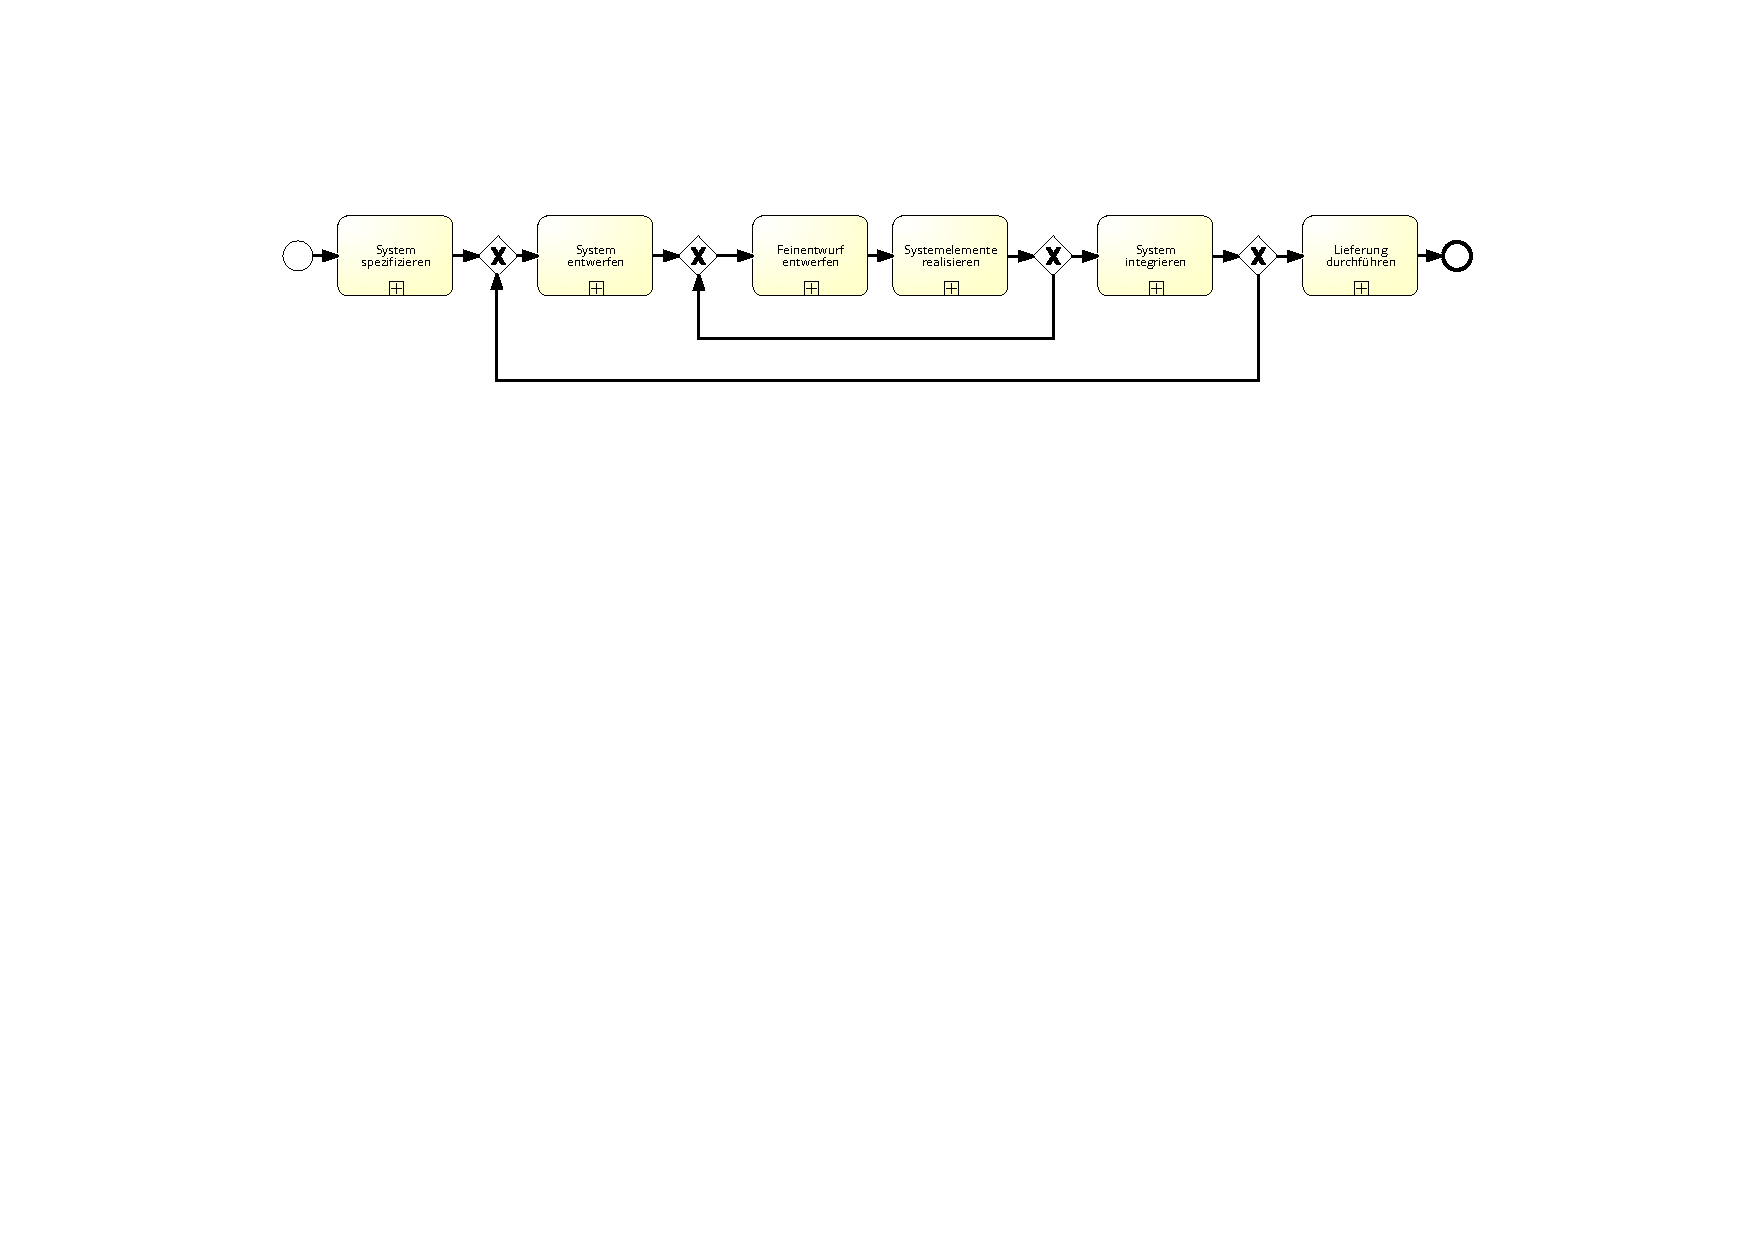
\includegraphics[width=\linewidth]{Inkrementell} %pdf, jpg, png...
  \caption{Unterprozess Inkrementelle Entwicklung durchführen V-Modell XT - imperativ}
  \label{fig:Inkrementell}
\end{center}
\end{figure}



\clearpage


\subsubsection{System entwerfen}

Abbildung \ref{fig:SystementwurfKlein} zeigt die imperative Modellierung des Unterprozesses \grqq System entwerfen\grqq.\newline
Die Aktivitäten \grqq Systemarchitektur erstellen, Unterstütungssystemarchitektur erstellen, Styleguide für die Mensch-Maschine-Schnittstelle erstellen, HW-Architektur erstellen, SW-Architektur erstellen, Datenbankentwurf erstellen, Implementierungs-, Integrations- und Prüfkonzept Unterstützungssystem erstellen, Integrations- und Prüfkonzept Hardware (HW) erstellen, Integrations- und Prüfkonzept Software (SW) erstellen\grqq \ und \grqq Migrationskonzept erstellen\grqq \ werden hier nacheinander ausgeführt.
\begin{sidewaysfigure}[!htbp]
\begin{center}
  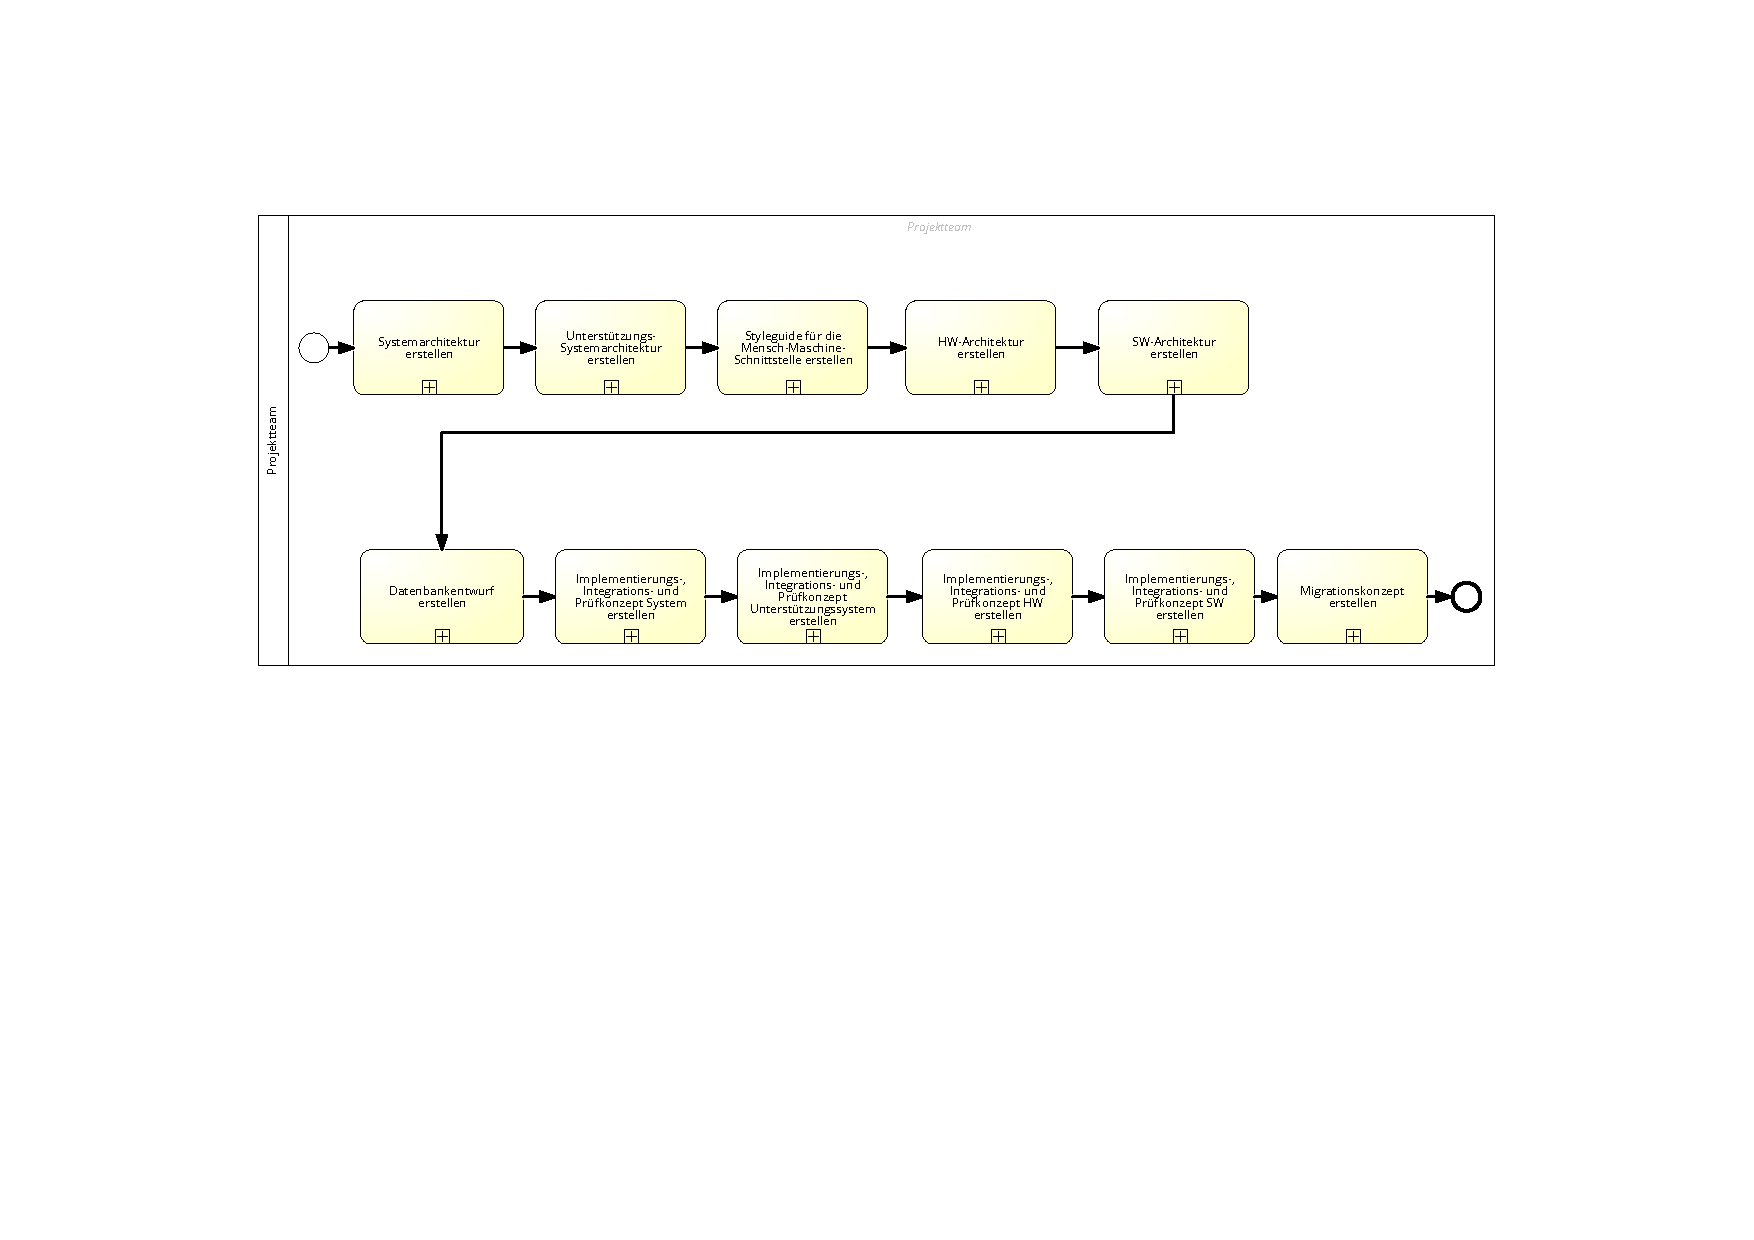
\includegraphics[width=\linewidth]{SystementwurfKlein} %pdf, jpg, png...
  \caption{System entwerfen V-Modell XT - imperativ}
  \label{fig:SystementwurfKlein}
\end{center}
\end{sidewaysfigure}


\subsubsection{System spezifizieren}

Zu Beginn des Unterprozesses \grqq System spezifizieren\grqq \  (Abbildung \ref{fig:BerichtswesenimpKlein}) muss eine \grqq Besprechung durchgeführt\grqq \  werden. Hieraus entsteht das Artefakt \grqq Besprechungsdokument\grqq.\newline
Parallel zu allen anderen Aktivitäten ist bei Bedarf bei jeder Änderung das \grqq Projekttagebuch zu führen\grqq. Dies wird durch das Parallel-Gateway sichergstellt und das Exklusive Gateway stellt sicher, dass die Akrtivität so oft durchgeführt wird, wie Anpassungen notwendig sind. \newline
Im nächsten Schritt werden die \grqq Messdaten erfasst\grqq.
In der nachfolgenden Aktivität wird die \grqq Metrik berechnet und ausgewertet\grqq, woraus das Artefakt \grqq Metrikauswertung\grqq \  entsteht.
Anschließend erfolgt die Durchführung der Aktivität \grqq Kaufmännischen Projektstausbericht erstellen\grqq, wobei das Artefakt \grqq {Kaufmännischer Projektstausbericht\grqq \  als Artefakt herauskommt.\newline
Bei der nächsten Aktivität wird der \grqq Projektstatusbericht erstellt\grqq \  und danach wird der \grqq Gesamtprojektfortschritt ermittelt\grqq.\newline
Die Aktivität \grqq QS-Bericht erstellen\grqq \  bringt dann das Artefakt \grqq QS-Bericht hervor\grqq \  und die nachfolgende Aktivität \grqq Projekt abschließen\grqq \  den \grqq Projektabschlußbericht\grqq.

\begin{sidewaysfigure}[!htp]
\begin{center}
  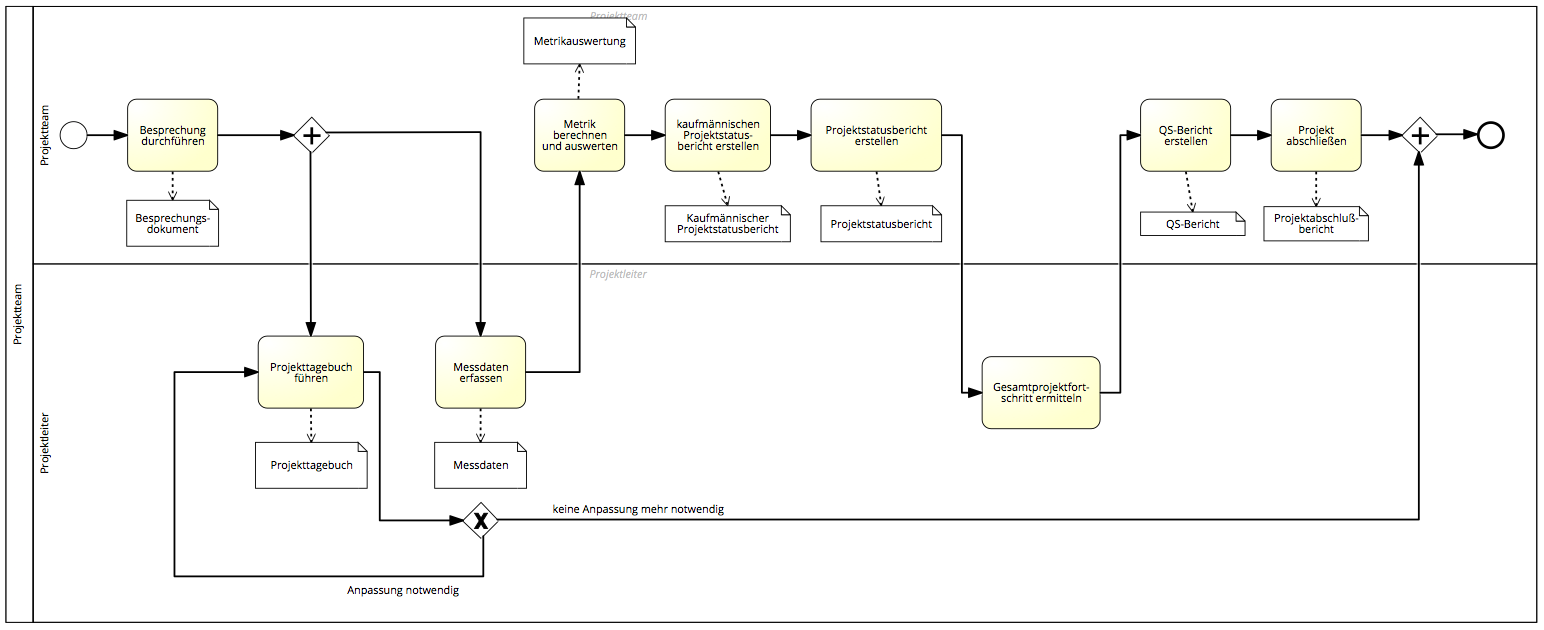
\includegraphics[width=\linewidth]{BerichtswesenimpKlein} %pdf, jpg, png...
  \caption{System spezifizieren-imperativ}
  \label{fig:BerichtswesenimpKlein}
  \end{center}
\end{sidewaysfigure}

\clearpage
\subsection{Deklarative Modellierung V-Modell XT}

Nachfolgend werden die entsprechenden deklarativen Modelle zu den imperativen Modellen modelliert.

\subsubsection{Systementwicklungsprojekt AG/AN}

Die deklarative Modellierung von \grqq Systementwicklungsprojekt AG/AN\grqq  zeigt Abbildung \ref{fig:SystemV}. \newline
Zunächst muss ein Projekt genehmigt und definiert werden. Dies ist durch die aufeinander folgenden Aktivitäten \grqq Projekt genehmigen\grqq \ und \grqq Projekt definieren\grqq \ dargestellt, welche durch das Constraint \textit{succession} verbunden sind.\newline
In der nachfolgenden Aktivität müssen sodann die \grqq Anforderungen festgelegt werden\grqq, bevor die \grqq Iteration geplant\grqq \ werden kann. \newline
Hiernach muss entschieden werden, ob eine \textit{Prototypische Entwicklung durchgeführt}, eine \textit{Komponentenbasierte Entwicklung durchgeführt} oder eine \grqq Inkrementelle Entwicklung durchgeführt\grqq \ werden soll. Dies wird hier durch den Unterprozess \grqq Entwicklung durchführen\grqq \ (Abbildung \ref{fig:SystemVUnter}) dargestellt, da dieser Sachverhalt auf Grund der Schleifen im Prozess ohne Unterprozess nicht darstellbar war. Im Unterprozess kann dann eine der drei Aktivitäten ausgeführt werden, was das Constraint \textit{1of 3} vorgibt.\newline
Anschließend wird das \grqq System abgenommen\grqq.
An dieser Stelle wird enschieden, ob erneut zu \grqq Anforderungen festlegen\grqq \ zurückgekehrt wird und der Prozess ab dieser Aktivität erneut startet oder ob zu \grqq Projekt ausschreiben\grqq \ zurückgekehrt wird und der Prozess ab hier erneut startet. Ansonsten endet der Prozess mit der Aktivität \grqq Projekt abschließen\grqq.

\begin{figure}[!htbp]
\begin{center}
  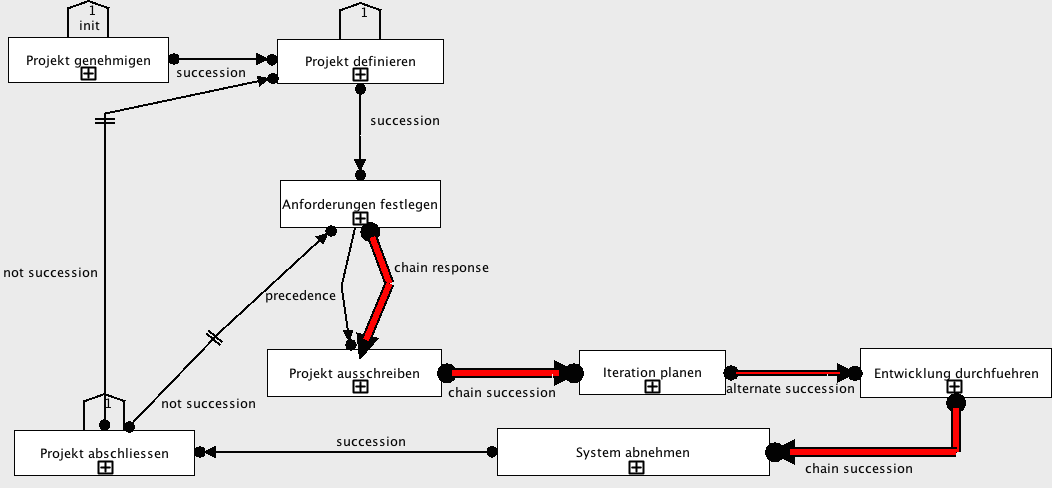
\includegraphics[width=\linewidth]{SystemV} %pdf, jpg, png...
  \caption{Systementwicklungsprojekt AG/AN  V-Modell XT - deklarativ}
  \label{fig:SystemV}
\end{center}
\end{figure}

\begin{figure}[!htbp]
\begin{center}
  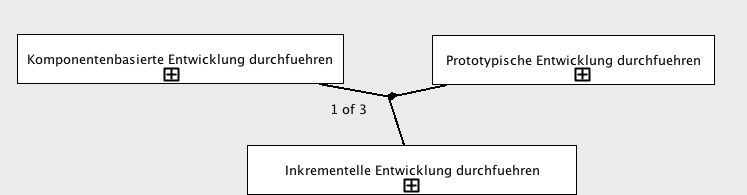
\includegraphics[scale=0.5]{SystemVUnter} %pdf, jpg, png...
  \caption{Systementwicklungsprojekt AG/AN  V-Modell XT Unterprozess Entwicklung durchführen - deklarativ}
  \label{fig:SystemVUnter}
\end{center}
\end{figure}



\subsubsection{Inkrementelle Entwicklung durchführen}
In Abbildung \ref{fig:Systementwicklung} ist die deklarative Modellierung des Unterprozesses \textit{Inkrementelle Entwicklung durchführen} abgebildet. \newline
Zu Beginn muss das \grqq System spezifiziert\grqq \ werden, weshalb diese Aktivität mit dem Constraint \textit{Init} beschrieben ist und anschließend wird das \textit{System entworfen}, was durch das Constraint \textit{succession} zwischen diesen beiden Aktivitäten sichergestellt wird.\newline
Hiernach wird der Feinentwurf entworfen und Systemelemente realisiert. Diese beiden Aktivitäten können so oft wie nötig durchgeführt werden. Es kommt nur darauf an, dass zuerst die Aktivität \grqq Feinentwurf entwerfen\grqq \ und anschließend die Aktivität \grqq Systemelemente realisieren\grqq \ durchgeführt wird, weshalb das Constraint \textit{chain succession} sich zwischen diesen beiden Aktivitäten befindet. \newline
Im nächsten Schritt wird das System integriert und es beginnt eine neue Iteration bei der Aktivität System entwerfen. Aus diesem Grund befindet sich hier das Constraint \textit{alternate succession} zwischen den Aktivitäten \grqq System integrieren\grqq \ und \grqq System entwerfen\grqq, da eine erneute Ausführung von \grqq System entwerfen\grqq \ erst nach Ausführung der Aktivität \grqq System integrieren\grqq \ möglich ist. \newline
Falls keine weitere Iteration mehr notwendig ist, wird die \grqq Lieferung durchgeführt\grqq \ und der Unterprozess endet hier, da durch die Constraints zu \grqq System entwerfen\grqq \ und \grqq Feinentwurf entwerfen\grqq \ keine weitere Aktivität mehr ausgeführt werden kann. \newline
\begin{figure}[!htbp]
\begin{center}
  \includegraphics[width=\linewidth]{Systementwicklung} %pdf, jpg, png...
  \caption{Unterprozess Inkrementelle Entwicklung durchführen V-Modell XT - imperativ}
  \label{fig:Systementwicklung}
\end{center}
\end{figure}



\subsubsection{System entwerfen}


Abbildung \ref{fig:SystementwurfKleinDec} zeigt die deklarative Modellierung von System entwerfen.\newline
Die Aktivitäten \grqq Systemarchitektur erstellen, Unterstütungssystemarchitektur erstellen, Styleguide für die Mensch-Maschine-Schnittstelle erstellen, HW-Architektur erstellen, SW-Architektur erstellen, Datenbankentwurf erstellen, Implementierungs-, Integrations- und Prüfkonzeptsystem erstellen, Implementierungs-, Integrations- und Prüfkonzeptunterstützungssystem erstellen, Implementierungs-, Integrations- und Prüfkonzept HW erstellen, Implementierungs-, Integrations- und Prüfkonzept SW erstellen\grqq \ und \grqq Migrationskonzept erstellen\grqq \ werden hier nacheinander ausgeführt. Da die vorherige Aktivität immer Voraussetzung für das Ausführen der nachfolgenden Aktivität ist, und die nachfolgende Aktivität nach der vorherigen ausgeführt werden muss, ist zwischen allen Aktivitäten jeweils \textit{succession} als Constraint eingefügt.

\begin{figure}[!htbp]
\begin{center}
  \includegraphics[width=\linewidth]{SystementwurfKleinDec} %pdf, jpg, png...
  \caption{System entwerfen - deklarativ}
  \label{fig:SystementwurfKleinDec}
\end{center}
\end{figure}

\subsubsection{System spezifizieren}


Zu Beginn von System spezifizieren (Abbildung \ref{fig:BerichtswesenKlein}) muss eine \textit{Besprechung durchgeführt} werden. Dies wird durch das Constraint \textit{init} sichergestellt. Bei jeder Änderung muss die Aktivität \grqq Projekttagebuch fuehren\grqq \ ausgeführt werden. Aus diesem Grund ist diese durch kein Constraint mit einer anderen Aktivität verbunden, da sie jederzeit ausgeführt werden kann und so oft wie nötig.
Im nächsten Schritt werden die \grqq Messdaten erfasst\grqq. Da ab hier alle Aktivitäten nacheinander auszuführen sind, sind dies jeweils durch das Constraint \textit{succession} verbunden.\newline
In der nachfolgenden Aktivität wird die \grqq Metrik berechnet und ausgewertet\grqq.\newline
Anschließend erfolgt die Durchführung der Aktivität \grqq Kaufmännischen Projektstatusbericht erstellen\grqq.\newline
Bei der nächsten Aktivität wird der \grqq Projektstatusbericht erstellt\grqq \ und danach wird der \grqq Gesamtprojektfortschritt ermittelt\grqq.
Danach werden noch die Aktivitäten \grqq QS-Bericht erstellen\grqq \ und \grqq Projekt abschließen\grqq \ ausgeführt.

\begin{figure}[!htbp]
\begin{center}
  \includegraphics[width=\linewidth]{BerichtswesenKlein} %pdf, jpg, png...
  \caption{System spezifizieren- deklarativ}
  \label{fig:BerichtswesenKlein}
\end{center}
\end{figure}

\clearpage

\subsection{Vergleich}


Abbildung \ref{fig:SystementwicklungsprojektExcel} zeigt die Zahl notwendiger Elemente zur Darstellung des Prozesses \grqq Systementwicklungsprojekt AG/AN\grqq. In ConDec (11 Aktivitäten) ist somit eine Aktivität mehr zur Darstellung nötig als in BPMN (10 Aktivitäten). In BPMN werden vier Gateways und 20 Sequenzflusselemente verwendet. In ConDec hingegen braucht es 11 Constraints. In ConDec werden sieben unterschiedliche Constraints im Modell verwendet in BPMN nur eines. Somit sind zur Darstellung des Sachverhaltes insgesamt 34 BPMN Elemente 25 ConDec Elemente notwendig.\newline

\begin{figure}[!htbp]
\begin{center}
  \includegraphics[scale=0.6]{SystementwicklungsprojektExcel} %pdf, jpg, png...
  \caption{Systementwicklungsprojekt AG/AN}
  \label{fig:SystementwicklungsprojektExcel}
\end{center}
\end{figure}

Die Anzahl der Elemente zur Darstellung des Prozesses \grqq Inkrementelle Entwicklung\grqq \ kann Abbildung \ref{fig:InkrementellExcel} entnommen werden. Es werden jeweils sechs Aktivitäten verwendet. Weiterhin werden in BPMN vier Gateways und 13 Sequenzflüsse zur Darstellung des Prozessablaufes benötigt. In ConDec sind hierfür neun Constraints und zwei Existenz-Constraints notwendig. BPMN benötigt ein Gateway, also keine verschiedenen Gateways und ConDec braucht sechs unterschiedliche Constraints. Somit ergeben sich in Summe 23 BPMN Elemente und 17 ConDec Elemente zur Darstellung des Sachverhaltes. \newline

\begin{figure}[!htbp]
\begin{center}
  \includegraphics[scale=0.6]{InkrementellExcel} %pdf, jpg, png...
  \caption{Inkrementelle Entwicklung}
  \label{fig:InkrementellExcel}
\end{center}
\end{figure}

Abbildung \ref{fig:SystementwurfExcel} zeigt die Anzahl der Elemente, welche zur Darstellung des Prozesses \grqq System entwerfen\grqq \ notwendig sind. Demnach werden in beiden Prozessmodellierungssprachen jeweils 11 Aktivitäten verwendet. In BPMN werden keine Gateways und 12 Sequenzflusselemente benötigt. ConDec braucht zur Darstellung des Sachverhaltes 10 Constraints und 11 Existenz-Constraints jedoch keine unterschiedlichen Constraints. In Summe sind somit in BPMN 23 Elemente und in ConDec 32 Elemente zur Darstellung notwendig.\newline

\begin{figure}[!htbp]
\begin{center}
  \includegraphics[scale=0.6]{SystementwurfExcel} %pdf, jpg, png...
  \caption{System entwerfen}
  \label{fig:SystementwurfExcel}
\end{center}
\end{figure}

In Abbildung \ref{fig:SpezifizierenExcel} ist die Anzahl der Elemente zur Darstellung des Prozesses \grqq System spezifizieren\grqq \ abgetragen. Demnach werden neun Aktivitäten verwendet sowohl in BPMN als auch in ConDec. Es werden drei Gateways und 15 Sequenzflüsse in BPMN benötigt. In ConDec werden acht Constraints und neun Existenz-Constraints zur Darstellung verwendet. Weiterhin gibt es zwei unterschiedliche Gateways in BPMN und zwei unterschiedliche Constraints in ConDec. Insgesamt ergeben sich somit 27 unterschiedliche Elemente in BPMN und 26 unterschiedliche Elemente in ConDec. \newline

\begin{figure}[!htbp]
\begin{center}
  \includegraphics[scale=0.6]{SpezifizierenExcel} %pdf, jpg, png...
  \caption{System spezifizieren}
  \label{fig:SpezifizierenExcel}
\end{center}
\end{figure}

Sowohl BPMN, als auch ConDec können die syntaktische \textit{Richtigkeit} jedoch einhalten, da in beiden Modellierungssprachen die Notationsregeln bei der Modellierung der Prozessmodelle eingehalten werden können[A 1.1] .\newline
Die semantische \textit{Richtigkeit} [A 1.2] kann von ConDec in Bezug auf die Darstellung von Rollen und Artefakten nicht eingehalten werden. Hier werden Grenzen der Darstellbarkeit in ConDec erreicht.\newline

 
Der  Grundsatz des \textit{systematischen Aufbaus} [A 2.1] kann bei ConDec wiederum nicht eingehalten werden, da keine Artefakte visualisiert werden können.\newline

Der Grundsatz der \textit{Relevanz} [A 3.1] kann wieder nur von BPMN eingehalten werden, da es bei den ConDec-Modellen keine Visualisierungsmöglichkeiten für Rollen und Artefakte gibt.\newline


Beim Grungsatz der \textit{Klarheit} gibt es Unterschiede zwischen den Modellen. Zur Darstellung der beiden Prozesse \grqq Systementwicklungsprojekt AG/AN\grqq \ und \grqq Inkrementelle Entwicklung\grqq \ werden in ConDec jeweils viele Constraints benötigt (11 bei Systementwicklungsprojekt AG/AN, 7 unterschiedliche und 9 bei Inkrementelle Entwicklung, 6 unterschiedliche). Im Hinblick auf Sequenzfluss/Existenz Constraints braucht es beim Prozess Systementwicklungsprojekt AG/AN 13 Sequenzflusselemente und drei Existenz Constraints und beim Prozess Inkrementelle Entwicklung 20 Sequenzflusselemente und zwei Existenz Constraints. Da BPMN bei diesen beiden Modellen in dem einfach gewichteten Punkt Sequenzfluss/Existenz komplexer ist, jedoch bei den beiden doppelt gewichteten Punkten Gateways/Constraints und unterschiedliche Gateways/Constraints ConDec komplexer ist, können die beiden BPMN Modelle das Kriterium [A 4.1] besser erfüllen.\newline
Beim Prozess \grqq Systementwurf\grqq \ werden bei ConDec 10 Constraints verwendet, in BPMN hingegen keine Gateways. BPMN weist bei dem einfach gewichteten Punkt Sequenzfluss/Existenz mehr Elemente auf und ConDec in den beiden doppelt gewichteten Punkten Gateways/Constraints und unterschiedliche Gateways/Constraints. Somit ist das ConDec Modell das insgesamt komplexere Modell [A 4.1].\newline
Beim Prozess \grqq System spezifizieren\grqq \ werden in BPMN drei Gateways verwendet und in ConDec acht Constraints. Bei beiden handelt es sich dabei um zwei unterschiedliche Gateways/Constraints. Da ConDec in dem doppelt gewichteten Punkt Gateways/Constraints eine höhere Anzahl aufweist und BPMN nur im einfach gewichteten Punkt Sequenzfluss/Constraints eine höhere Anzahl aufweist, ist das mit BPMN erstellte Modell hier das verständlichere [A 4.1]. \newline
Bei den vier Modellen haben sowohl die in ConDec erstellten, als auch die in BPMN erstellten Modelle alle einen eindeutigen Startpunkt, wodurch Kriterium [A4.2] bei allen Modellen erfüllt ist.\newline
Somit lässt sich insgesamt festhalten, dass beim Grundsatz der \textit{Klarheit} BPMN hier die geeignetere Modellierungssprache ist, da sie weniger komplexe Modelle erzeugt und somit Kriterium [A 4.1] besser erfüllt.\newline

Die Anzahl der Elemente insgesamt unterscheidet sich bis auf das Modell \grqq Systemetwicklungsprojekt AG/AN\grqq \ nicht stark voneinander. Die BPMN-Modelle weisen eine höhere Anzahl an Sequenzflusselementen auf, als die ConDec Modelle Existenz- Constraints aufweisen
Der Grundsatz der \textit{Wirtschaftlichkeit} kann von BPMN besser eingehalten werden, da die ConDec Modelle deutlich mehr Constraints und auch verschiedene Constraints enthalten und somit ein größerer geistiger Aufwand für die Erstellung der Modelle aufgebracht werden muss.\newline


Bei Ausführung der Prozesse in den Modellierungstools Signavio und Declare weisen beide das gleiche Ausführungsverhalten auf, wodurch die \textit{Vergleichbarkeit} gewährleistet ist [A 6.1]. \newline
Die Anzahl der Elemente in den Prozessmodellen unterscheidet sich teilweise. Bei BPMN werden bei den Prozessen \grqq Systementwicklungsprojekt AG/AN\grqq \ deutlich mehr Elemente zur Darstellung des gleichen Sachverhaltes verwendet wie bei ConDec. Beim Prozess \grqq Systementwurf\grqq \ werden bei ConDec mehr Elemente benötigt wie bei BPMN und bei System spezifizieren werden in etwa gleich viele Elemente verwendet [A 6.2].\newline
Die \textit{Vergleichbarkeit} kann jedoch in Bezug auf Artefakte und Rollen [A 6.3], außer bei den Phasen des Open UP (hier werden noch keine Artefkate und Rollen verwendet) nicht eingehalten werden.\newline
Somit weisen bei der \textit{Vergleichbarkeit} beide Prozessmodellierungssprachen Stärken und Schwächen auf. ConDec kann [A 6.2] besser einhalten und BPMN [A 6.3]. [A 6.1] kann sowohl von ConDec, als auch von BPMN gleichermaßen eingehalten werden. \newline
Abbildung \ref{fig:TabelleVModell} gibt nochmal eine zusammenfassende Übersicht über die Ergebnisse des Vergleichs. 


\begin{figure}[!htbp]
\begin{center}
  \includegraphics[scale=0.6]{TabelleVModell} %pdf, jpg, png...
  \caption{Übersicht Vergleich V-Modell XT}
  \label{fig:TabelleVModell}
\end{center}
\end{figure}


\section{Übergreifender Vergleich}

BPMN und ConDec können die syntaktische \textit{Richtigkeit} [A 1.1] bei allen Modellen einhalten, da in beiden Modellierungssprachen die Notationsregeln bei der Modellierung der Metamodelle eingehalten werden können, um das dort beschriebene Verhalten korrekt wieder zu geben. Somit sind in Bezug auf die syntaktische \textit{Richtigkeit} beide Prozessmodellierungssprachen gleich geeignet.\newline
Die semantische \textit{Richtigkeit} [A 1.2] kann von ConDec in Bezug auf die visuelle Darstellung von Rollen und Artefakten im Prozessmodell selbst bei keinem Modell eingehalten werden, bei welchem solche Informationen notwendig wären. Die Grenzen der Darstellbarkeit von ConDec  werden erreicht. \newline
Da BPMN die beiden Kriterien [A 1.1] und [A 1.2] einhalten kann und ConDec das Kriterium [A 1.2] nicht einhalten kann, ist BPMN in Bezug auf \textit{Richtigkeit} die geeignetere Modellierungssprache. \newline


Der  Grundsatz des \textit{systematischen Aufbaus} [A 2.1] kann bei ConDec bei keinem Prozessmodell eingehalten werden, da niergendwo Artefakte visualisiert werden können. Da Artefakte jedoch für das Verständnis eines Modelles und die Darstellung von Schnittstellen sehr wichtige Elemente sind, ist BPMN in Hinsicht auf den \textit{systematischen Aufbau} die geeignetere Prozessmodellierungssprache. \newline


Die \textit{Relevanz} [A 3.1] kann ebenfalls nur von BPMN eingehalten werden, da sich die ConDec-Modelle nicht mit den minimal relevanten Informationen erstellen lassen. Auch ist das Problem wiederum die fehlende Visualisierungsmöglichkeit von Rollen und Artefakten. Somit ist auch hier BPMN die geeignetere Prozessmodellierungssprache.\newline

Beim Grungsatz der \textit{Klarheit} gibt es Unterschiede bei der Eignung zwischen den beiden Prozessmodellierungssprachen abhängig vom abzubildenden Verhalten des Metamodelles. Hier weisen beide Modelle Stärken und Schwächen auf. \newline
Bei der Darstellung von Metamodellen, bei denen viele Aktivitäten parallel ablaufen, wie z.B. bei den Phasen des Open UP, benötigt BPMN deutlich mehr Elemente zur Darstellung, als ConDec. Auch sind in BPMN Gateways zur Darstellung notwendig, während bei ConDec lediglich leichter verständliche Existenz-Constraints eingesetzt werden [A 4.1]. Dies ist sowohl der Fall bei den kleineren Modellen ( kleiner hier definiert als <=fünf Aktivitäten), als auch bei den größeren Modellen(größer hier definiert als >fünf Aktivitäten). Somit sind die BPMN Modelle komplexer als die ConDec Modelle und ConDec ist hierfür die geeignetere Prozessmodellierungssprache im hinblick auf [A 4.1] und [A 4.3]. \newline
Ein anderes Bild zeichnet sich bei Prozessmodellen ab, bei welchen viele Verzweigungen oder aber auch Abläufe ohne Verzweigungen und Parallelität, also gerade Abläufe dargestellt werden müssen. Hier werden bei BPMN bei der Darstellung von Abläufen ohne Verzweigung keine Gateways und bei der Darstellung von Abläufen mit vielen Verzweigungen auch maximal zwei verschiedene Gateways benötigt. ConDec braucht zur Darstellung von Abläufen ohne Verzweigung und Parallelität trotzdem Constraints, wenn auch wenig unterschiedliche [A 4.1]. Zur Darstellung von Abläufen mit vielen Verzweigungen/Schleifen und auch eventuell noch gleichzeitig parallelen Abläufen werden bei ConDec viele unterschiedliche Constraints eingesetzt. Bei kleinen Modellen (<= fünf Aktivitäten), wie z.B. beim Modell \grqq Phasen des Open UP\grqq \ ist ConDec das weniger komplexe Modell. Beim Prozess \grqq Lösungsinkrement entwickeln\grqq \ ist nur ein kleiner Unterschied in der Komplexität vorhanden. Bei größeren Modellen (>fünf Aktivitäten) sind jedoch die ConDec Modelle deutlich komplexer. Dies lässt sich bei den Modellen Scrum sowie bei den beiden Modellen des V-Modell XT \grqq Systementwicklungsprojekt AG/AN\grqq \ und \grqq Inkrementelle Entwicklung\grqq \ erkennen. Hier müssen bei den ConDec Modellen vier bis sieben unterschiedliche Constraints zur Darstellung des Ablaufes verwendet werden. In BPMN hingegen werden bei diesen Modellen maximal zwei unterschiedliche Gateways verwendet. Daher ist bei Modellen mit mehr als fünf Aktivitäten und vielen Verzweigungen und eventuell noch parallelen Aktivitäten BPMN die geeignetere Modellierungssprache im Hinblick auf die rfüllung von [A 4.1] und [A 4.3]. Hingegen bei Prozessen mit vielen parallelen Aktivitäten ist ConDec kann ConDec [A 4.1] und [A 4.3] besser erfüllen.\newline

Bei Betracht der \textit{Wirtschaftlichkeit} weisen beide Modellierungssprachen Stärken und Schwächen auf. Bei Modellen mit vielen parallelen Abläufen, wie z.B. den Phasen des Open UP müssen in BPMN mehr Gateways und Gequenzflusselemente verwendet werden, wie bei ConDec, wodurch ein höherer Aufwand bei der Modellierung mit BPMN entsteht als bei ConDec [A 5.1].\newline
Bei großen Modellen (>fünf Aktivitäten) mit vielen Verzweigungen/Schleifen und noch dazu parallelen Aktivitäten werden bei ConDec sehr viel mehr Constraints bei der Modellierung benötigt, als Gateways bei BPMN. Aus diesem Grund ist bei diesen Modellen bei der Modelierung mit ConDec ein größerer geistiger Aufwand notwendig als bei BPMN und daher ist bei Modellen mit vielen Verzweigungen/Schleifen BPMN die geeignetere Modellierungssprache, wenn die \textit{Wirtschaftlichkeit} betrachtet wird [A 5.1 und A 5.2].\newline
Bei kleinen Modellen mit vielen parallelen Aktivitäten hingegen ist ConDec geeigneter, da die Modelle weniger komplex zu modellieren sind [A 5.1 und A 5.2].\newline


Bei allen Prozessen lässt sich durch Ausführung in den Modellierungstools Signavio und Declare das gleiche Ausführungsverhalten beobachten, wodurch hier die \textit{Vergleichbarkeit} [A 6.1] gewährleistet ist. \newline
Die Anzahl der Elemente in den Prozessmodellen [A 6.2] unterscheidet sich teilweise. Bei BPMN werden bei vielen Prozessen deutlich mehr Elemente zur Darstellung des gleichen Sachverhaltes verwendet wie bei ConDec.\newline
Die \textit{Vergleichbarkeit} kann jedoch in Bezug auf Artefakte und Rollen, außer bei den Phasen des Open UP (hier werden noch keine Artefakte und Rollen verwendet) nicht eingehalten werden [A 6.3].\newline
Somit weisen bei der \textit{Vergleichbarkeit} beide Prozessmodellierungssprachen Stärken und Schwächen auf. ConDec kann das Kriterium [A 6.2] erfüllen und BPMN das Kriterium [A 6.3]. Das Kriterium [A 6.1] kann von beiden Modellierungssprachen eingehalten werden. \newline


Abbildung \ref{fig:TabelleAllgemein} gibt nochmal eine zusammenfassende Übersicht über die Ergebnisse des Vergleichs. 



 \begin{figure}[!htbp]
\begin{center}
  \includegraphics[width=\linewidth]{TabelleAllgemein} %pdf, jpg, png...
  \caption{Übersicht Vergleich Allgemein}
  \label{fig:TabelleAllgemein}
\end{center}
\end{figure}






